% -*- LaTeX -*-

% PLEASE USE THIS FILE AS A TEMPLATE FOR THE DOCUMENTATION OF YOUR OWN
% FACILITIES: IN PARTICULAR, IT IS IMPORTANT TO NOTE COMMENTS MADE IN
% THE TEXT AND TO FOLLOW THIS ORDERING. THE FORMAT FOLLOWS ONE USED BY
% THE COBE-DMR PROJECT.	
% A.J. Banday, April 1999.

\documentclass[12pt,twoside]{article}
% \usepackage{healrut,psfig,html,makeidx}
%\usepackage{healpix,psfig,html,makeidx}
%\usepackage{healpix,graphicx,html,makeidx}
\usepackage{healpix,graphicx,html,makeidx}
%\usepackage{hyperref,healpix,graphicx,html,makeidx}%putting hyperref first
%screws up references in html
%%%%%% ----- HTML only commands -------
\begin{htmlonly}
\renewcommand{\ell}{l}
\renewcommand{\lq}{'}
% -*- LaTeX -*-
% This LaTeX file sets the Healpix version
% as it will appear in the documentation
% implement it with: % -*- LaTeX -*-
% This LaTeX file sets the Healpix version
% as it will appear in the documentation
% implement it with: % -*- LaTeX -*-
% This LaTeX file sets the Healpix version
% as it will appear in the documentation
% implement it with: \input{hpxversion}
% \newcommand{\hpxversion}{3.31}
% \newcommand{\hpxverstex}{3\_31}
% \newcommand{\hpxversion}{3.40}
% \newcommand{\hpxverstex}{3\_40}
% \newcommand{\hpxversion}{3.41}
% \newcommand{\hpxverstex}{3\_41}
\newcommand{\hpxversion}{3.50}
\newcommand{\hpxverstex}{3\_50}

% \newcommand{\hpxversion}{3.31}
% \newcommand{\hpxverstex}{3\_31}
% \newcommand{\hpxversion}{3.40}
% \newcommand{\hpxverstex}{3\_40}
% \newcommand{\hpxversion}{3.41}
% \newcommand{\hpxverstex}{3\_41}
\newcommand{\hpxversion}{3.50}
\newcommand{\hpxverstex}{3\_50}

% \newcommand{\hpxversion}{3.31}
% \newcommand{\hpxverstex}{3\_31}
% \newcommand{\hpxversion}{3.40}
% \newcommand{\hpxverstex}{3\_40}
% \newcommand{\hpxversion}{3.41}
% \newcommand{\hpxverstex}{3\_41}
\newcommand{\hpxversion}{3.50}
\newcommand{\hpxverstex}{3\_50}

% -*- LaTeX -*-
% This LaTeX file sets the IDL version required to run Healpix-DL
% as it will appear in the documentation
% implement it with: % -*- LaTeX -*-
% This LaTeX file sets the IDL version required to run Healpix-DL
% as it will appear in the documentation
% implement it with: % -*- LaTeX -*-
% This LaTeX file sets the IDL version required to run Healpix-DL
% as it will appear in the documentation
% implement it with: \input{idlversion}
%\newcommand{\idlversion}{5.6 }
%\newcommand{\idlversion}{6.0 }
\newcommand{\idlversion}{6.1 }

%\newcommand{\idlversion}{5.6 }
%\newcommand{\idlversion}{6.0 }
\newcommand{\idlversion}{6.1 }

%\newcommand{\idlversion}{5.6 }
%\newcommand{\idlversion}{6.0 }
\newcommand{\idlversion}{6.1 }

\end{htmlonly}

\hypersetup{%
	pdftitle={HEALPix IDL Overview},%
	pdfauthor={E. Hivon et al},%
	pdfkeywords={HEALPix, IDL},%
	colorlinks=true}

%%%%%% ----- commands for HTML and PDF -----
\newcommand{\nside}{{N_{\rm side}}}
\newcommand{\npix}{{N_{\rm pix}}}
\newcommand{\ntemplate}{{N_{\rm template}}}
%\newcommand{\myhtmlimage}[1]{\htmlimage{#1}}
\newcommand{\myhtmlimage}[1]{ }
\renewcommand{\contentsname}{{TABLE OF CONTENTS}}
% command for external link
\newcommand{\linklatexhtml}[3]{% \linklatexhtml{name}{latex_target}{html_target}
\latexhtml{\htmladdnormallink{#1}{#2}}{\htmladdnormallink{#1}{#3}}}
% commands for arbitrary link
\newcommand{\mylink}[2]{% \mylink{link_id}{link_text}
\latexhtml{\hyperlink{#1}{#2}}{\hyperref{#2}{}{}{#1}}}
\newcommand{\mytarget}[1]{% \mytarget{link_id}
\latexhtml{\hypertarget{#1}{}}{\label{#1}}}
\newcommand{\mytargetb}[2]{% \mytargett{link_id}{target_txt}
\latexhtml{\hbox{{#2}\hypertarget{#1}{}}}{\label{#1}{#2}}}

\newcommand{\facname}{}
\newcommand{\FACNAME}{}
%\renewcommand{\contentsname}{{TABLE OF CONTENTS\\\rule{\hsize}{0.7mm}\\}}

\sloppy
\setcounter{secnumdepth}{0}
\setcounter{tocdepth}{10}


\begin{document}
\title{\healpix IDL Facilities Overview}
\label{idl:idlxxx}
\docrv{Version \hpxversion}
\author{Eric Hivon, Anthony J.~Banday, Benjamin D.~Wandelt, Frode
K.~Hansen and Krzysztof M.~G\'orski}
\abstract{This document is an overview of the \healpix IDL facilities.}
\date{\today}

\frontpage
\tableofcontents
\newpage

\section{Using the \healpix IDL facilities}

%Before the \healpix IDL facilities can be utilised, the user MUST 
%install \hfill\newline

%\noindent {\it The IDL Astronomy User's Library} \hfill\newline
%\noindent (available for download at {\tt http://idlastro.gsfc.nasa.gov/homepage.html})\hfill\newline
%\noindent the {\it COBE (IDL) Analysis Software} \hfill\newline
%\noindent (available for download at {\tt http://space.gsfc.nasa.gov/astro/cobe/cgis.html}).\hfill\newline

%The \healpix developers are in no way associated with the
%contents of these packages, and any problems therewith should be
%directed to the respective providers. Having downloaded these
%packages, the user must update his environment variable {\tt
%IDL\_PATH} to add these directories.

%\vspace{5mm}
The current version of the \healpix package provides
an IDL startup file which defines various environment
variables for your convenience, and adds the \healpix
IDL directory tree to your {\tt IDL\_PATH}. In order to utilise
this feature, the user should invoke IDL using the
commands {\tt hidl} or {\tt hidlde} which are aliases defined in the
\healpix profile created during the installation process 
for the package.


\section{Changes between release 2.0 and 2.15a}
Several routines have been added or improved since version 2.0, as listed below.
Note that thanks to the newer {\tt IDL-astron} library, FITS read/write routines
in IDL-Healpix routines can now deal with {\bf FITS files larger than 2GB} (on architectures supporting 64bit
addressing).\\
Using 64 bit integers available since version 5.2 of IDL the maximum resolution parameter Nside supported has increased
from $2^{13}=8192$ to $2^{29}=536870912$, corresponding to $3.46\ 10^{18}$
pixels on the sphere.

\begin{itemize}
\item Recent editions (versions 2.15 and 2.15a)
\begin{itemize}
	\item \htmlref{{\tt cartview, gnomview, mollview, orthview}}{idl:mollview}:
        \begin{itemize} 
		\item export of projected map into a FITS file (\mylink{idl:mollview:fits}{{\tt FITS}} keyword), or an
IDL array (\mylink{idl:mollview:fits}{{\tt MAP\_OUT}} option) now available with all viewing routines,
		\item added \mylink{idl:mollview:charthick}{{\tt CHARTHICK}} support; accept array of \mylink{idl:mollview:outline}{{\tt
OUTLINE}} structures (if they have the same fields),
		\item correction of a bug (in {\tt loaddata\_healpix}) that was
affecting the behavior of these viewing routines after consecutive calls with
very partial cut-sky {\em and then} full-sky data sets [2.15a];
	\end{itemize}
	\item \htmlref{{\tt remove\_dipole}}{idl:remove_dipole} now outputs the monopole and dipole
\mylink{idl:remove_dipole:covariance_matrix}{covariance matrix};
	\item 
\htmlref{{\tt write\_fits\_map}}{idl:write_fits_map}, 
\htmlref{{\tt write\_tqu}}{idl:write_tqu}, 
\htmlref{{\tt write\_fits\_sb}}{idl:write_fits_sb}: {\tt
BAD\_DATA} keyword added to FITS header;
        \item update of {\tt astron} library routines (24-May-2010) for improved WCS support.
\end{itemize}


\item Previous edition (version 2.14a)
 \begin{itemize}
	\item \htmlref{{\tt cartview, gnomview, mollview, orthview}}{idl:mollview}:
        \begin{itemize}
		\item {\tt OUTLINE=}, {\tt GRATICULE=}, {\tt IGRATICULE=} work
again with virtual windows ({\tt WINDOW}$<0$)
		\item {\tt YPOS=} and {\tt RETAIN=} keywords active again
		\item {\tt PS=} keyword fixed % 2.14a
	\end{itemize}
	\item \htmlref{{\tt orthview}}{idl:mollview}:
		fixed problems with {\tt /SHADE} keyword, which now
outputs 8-byte (instead of 16-byte) PNG files
	\item \htmlref{{\tt ianafast}}{idl:ianafast}, 
		\htmlref{{\tt ismoothing}}{idl:ismoothing}: 
	fixed problem with processing of
polarized maps stored in memory.
	\item \htmlref{{\tt ud\_grade}}{idl:ud_grade}: 
	improved handling of flagged pixels on Double
Precision input maps
	\item \htmlref{{\tt remove\_dipole}}{idl:remove_dipole}: 
{\tt COORD\_IN=} and {\tt COORD\_OUT=} now
accept lower case values; {\tt /SILENT} keyword added.
 \end{itemize}
%
%
%
%--------------------------------
\end{itemize}
{\footnotesize{%
\begin{itemize}
%--------------------------------
\item Old edition (version 2.13)
   \begin{itemize}
	\item new \htmlref{{\tt healpix\_doc}}{idl:healpix_doc} routine to
browse HTML and PDF documentations
	\item \htmlref{{\tt cartview, gnomview, mollview, orthview}}{idl:mollview}:
        \begin{itemize}
		\item introduction of the {\tt TRUECOLORS=} keyword to generate
color image from 3 channel map
		\item extended capability of the {\tt TRANSPARENT=} keyword
		\item addition of {\tt MAP\_OUT=} to {\tt gnomview}
	\end{itemize}
	\item improved compatibility with 
\htmladdnormallink{GDL}{http://gnudatalanguage.sourceforge.net}
 (free IDL clone). See \linklatexhtml{``\healpix Installation Document''}{install.pdf}{install.htm} for current GDL limitations.
	\item update of the {\tt IDL-astron} library routines, which now require IDL 6.1 or more
	\item \htmlref{{\tt fits2alm}}{idl:fits2alm}: new {\tt LMAX=} and {\tt LMIN=} keywords
	\item \htmlref{{\tt fits2cl}}{idl:fits2cl}: new {\tt LLFACTOR=}  keyword
	\item \htmlref{{\tt init\_healpix}}{idl:init_healpix} defines
substructure with complete path to \healpix subdirectories (test, data, bin)
	\item slightly faster \htmlref{{\tt write\_fits\_cut4}}{idl:write_fits_cut4}
	and \htmlref{{\tt write\_fits\_sb}}{idl:write_fits_sb} routines.
	%\item new alm\_i2t
	\item \htmlref{{\tt ianafast}}{idl:ianafast}, 
              \htmlref{{\tt ismoothing}}{idl:ismoothing}: solved problem with {\tt
W8DIR=} keyword.
   \end{itemize}

\item Older editions (versions 2.11 and 2.12a)
   \begin{itemize}
	\item \htmlref{{\tt ianafast}}{idl:ianafast}, 
              \htmlref{{\tt ismoothing}}{idl:ismoothing}, 
              \htmlref{{\tt isynfast}}{idl:isynfast}: the {\tt
TMPDIR} keyword now works properly, and {\tt \$IDL\_TMPDIR} is used as the
default temporary directory ; more stable behaviour of these routines
	\item \htmlref{{\tt ud\_grade}}{idl:ud_grade}: 
	\begin{itemize} 
		\item correctly flags bad output pixels with {\tt bad\_data}
value when upgrading maps
		\item cut sky map: improved, faster routine, now works for Nside $>$
8192
	\end{itemize}
	\item \htmlref{{\tt cartview, gnomview, mollview, orthview}}{idl:mollview}:
        \begin{itemize}
		\item using a virtual window (ie, setting {\tt WINDOW} to a
negative value) now allows faster generation of GIF and PNG files (especially useful over remote connections); 
		\item addition of {\tt RETAIN=} keyword; 
		\item deals correctly with user provided  {\tt MIN} and {\tt MAX} in
{\tt LOG} and {\tt ASINH} modes
		\item polarization norm map can be offset ({\tt POLARIZATION=1} mode)
		\item original color table and plot settings are restored when
leaving these routines
	\end{itemize}
	\item \htmlref{{\tt orthview}}{idl:mollview}: addition of 
              %\htmlref{{\tt /SHADED}}{kw:mol_shaded} 
              {\tt /SHADED}
	keyword for 3D rendering
	\item issues warning when non-integer pixel indexes are fed to \htmlref{{\tt nest2ring, ring2nest, pix2ang\_*, pix2vec\_*,}}{idl:pix_tools}   ...
	\item {\tt ximview}:
		\begin{itemize}
		\item fixed problem with cut-sky FITS files
		\item color scale bar added to PNG output
		\item version 0.6.2, fixed bug in pixel coordinates
		\end{itemize}
	\item cosmetic editions to {\tt remove\_dipole}
   \end{itemize}

%
\item New routines in version 2.10 include
\begin{itemize}
 \item {{\tt ximview}}: visualisation routine developed by J. P. Leahy intended for quick-look inspection of HEALPix images 
(as well as ordinary 2-D images) at the level of individual pixels. Features
include panning, zooming, blinking, image statistics and peak finding.
 \item \htmlref{{\tt hpx2gs}}{idl:hpx2gs}: turns a healpix data set into a
\htmladdnormallink{Google Earth}{http://earth.google.com/}%
/%
\htmladdnormallink{Google Sky}{http://earth.google.com/sky/skyedu.html}%
-compatible image
 \item \htmlref{{\tt ianafast}}{idl:ianafast}: interface to (F90) {\tt anafast}
and (C++) {\tt anafast\_cxx} facilities 
 \item \htmlref{{\tt isynfast}}{idl:isynfast}: interface to F90 {\tt synfast} facility
 \item \htmlref{{\tt ismoothing}}{idl:ismoothing}: interface to F90 {\tt smoothing} facility
 \item \htmlref{{\tt bin\_llcl}}{idl:bin_llcl}: $C(l)$ binning
 \item \htmlref{{\tt bl2fits}}{idl:bl2fits}: writes $B(l)$ or $W(l)$ window into
FITS file
 \item \htmlref{{\tt neighbours\_nest}}{idl:neighbours_nest}, %
       \htmlref{{\tt neighbours\_ring}}{idl:neighbours_ring}: %
   find immediate neighbours of a given pixel
 \item \htmlref{{\tt query\_strip}}{idl:query_strip}: %
   find pixels lying within a colatitude strip
\end{itemize}	
%
\item Routines with extended/improved user interface or new functionalities include
\begin{itemize}
\item \htmlref{{\tt mollview, gnomview, cartview, orthview}}{idl:mollview}: 
\begin{itemize}
\item {\tt ONLINE} keyword is now redundant, 
\item introduction of {\tt GLSIZE} and {\tt IGLSIZE} to
  	control automatic labeling of graticules,
	see Fig.~\ref{fig:plot_example_execute} on page~\pageref{page:plot_example_execute}
\item addition of {\tt SILENT} and {\tt EXECUTE} keywords,
	see Fig.~\ref{fig:plot_example_execute} on
	page~\pageref{page:plot_example_execute}
\item addition of {\tt ASINH} keyword to allow better visualisation of highly
contrasted maps; see Figure~\ref{fig:merge_wmapKband} on page~\pageref{page:merge_wmapKband},
\item under certain circumstances, can process high resolution cut sky data sets
	without creating full sky dummy maps,
\item accept gzip compressed FITS files,
\item accept polarized cut sky maps,
\item accept multi-dimensional online arrays,
\item more robust {\tt OUTLINE} option.
\end{itemize}

\item \htmlref{{\tt median\_filter}}{idl:median_filter}: bugs correction
\item \htmlref{{\tt ud\_grade}}{idl:ud_grade}: more robust user interface
\item \htmlref{{\tt change\_polcconv}}{idl:change_polcconv}: new {\tt /FORCE} keyword
\item \htmlref{{\tt remove\_dipole}}{idl:remove_dipole}: more accurate
\item \htmlref{{\tt query\_disc}}{idl:query_disc}: when the disc center is
located at one of
the poles, {\em only} the pixels overlapping with the disc are now returned.
\end{itemize}
%
\item Miscellaneous
\begin{itemize}
\item \htmlref{{\tt mollcursor, gnomcursor...}}{idl:mollcursor}: an X11 patch is
given so that these routines work under Mac OS X 10.4 and 10.5.
\end{itemize}
\end{itemize}

\section{Changes between release 1.2 and 2.0}
Some new routines have been introduced since version 1.2, as listed below.
Most of the routines that already existed now have extended
capabilities.
Those of them with improved or extended user interface are listed
below. They all remain backward compatible (ie, they can be used with codes written
around version 1.1 and 1.2 without any edition).

\begin{itemize}
\item New routines in version 2.0 include
\begin{itemize}
 \item \htmlref{{\tt median\_filter}}{idl:median_filter}
 \item \htmlref{{\tt nside2templates}}{idl:nside2ntemplates},
  \htmlref{{\tt same\_shape\_pixels\_ring}}{idl:same_shape_pixels_xxx}, 
  \htmlref{{\tt same\_shape\_pixels\_nest}}{idl:same_shape_pixels_xxx},
  \htmlref{{\tt template\_pixel\_ring}}{idl:template_pixel_xxx}, 
  \htmlref{{\tt template\_pixel\_nest}}{idl:template_pixel_xxx}
 \item {\tt loaddata\_healpix}: replaces loaddata to avoid conflict with other
  libraries
 \item \ldots
\end{itemize}

\item Routines with extended/improved user interface or new functionalities include
\begin{itemize}
\item \htmlref{{\tt fits2cl}}{idl:fits2cl}: addition of /RSHOW, /SHOW keywords to plot
  power spectra while they are read; possibility to read power spectra from a
file containing $a_{lm}$ coefficients.
\item \htmlref{{\tt gnomview}}{idl:mollview}, \htmlref{{\tt mollview}}{idl:mollview},
  \htmlref{{\tt orthview}}{idl:mollview}, \htmlref{{\tt cartview}}{idl:mollview}
  faster FITS file reading (by up to a factor 6);
  can deal with WMAP polarized maps FITS format; extension
  of the OUTLINE keyword to plot set of points; addition of the HBOUND keyword
  to overplot pixel boundaries; ...
\item \htmlref{{\tt read\_tqu}}{idl:read_tqu},
  \htmlref{{\tt read\_fits\_cut4}}{idl:read_fits_cut4},
  \htmlref{{\tt read\_fits\_map}}{idl:read_fits_map}: 
   addition of output keywords   NSIDE, ORDERING, COORDSYS
\item \htmlref{{\tt reorder}}{idl:reorder}: simpler interface to ordering
  conversion with addition of /N2R and /R2N keywords
\item \htmlref{{write\_tqu}}{idl:write_tqu},
\htmlref{{write\_fits\_cut4}}{idl:write_fits_cut4},
	\htmlref{{write\_fits\_sb}}{idl:write_fits_sb}: faster FITS file writing
(by a factor 10 or more);
\item \ldots
\end{itemize}
%--------------------------------
\end{itemize}
}} %% end of footnotesize
%--------------------------------


%% \section{Changes between release 1.1 and 1.2}
%% Some new routines have been introduced since version 1.1, as listed below.
%% Most of the routines that already existed now have extended
%% capabilities.
%% Those of them with improved or extended user interface are listed
%% below. They all remain backward compatible (ie, they can be used with codes written
%% around version 1.1 without any edition).

%% \begin{itemize}
%% \item New routines in version 1.2
%% \begin{itemize}
%% \item \htmlref{cartcursor}{idl:cartcursor}
%% \item \htmlref{cartview}{idl:cartview}
%% \item \htmlref{euler\_matrix\_new}{idl:euler_matrix_new} (replaces euler\_matrix)
%% \item \htmlref{getsize\_fits}{idl:getsize_fits}
%% \item \htmlref{init\_healpix}{idl:init_healpix}
%% \item \htmlref{orthcursor}{idl:orthcursor}
%% \item \htmlref{orthview}{idl:orthview}
%% \item \htmlref{query\_disc}{idl:query_disc} (replaces \htmlref{getdisc\_ring}{idl:getdisc_ring})
%% \item \htmlref{query\_polygon}{idl:query_polygon}
%% %%% \item query\_strip
%% \item \htmlref{query\_triangle}{idl:query_triangle}
%% \item \htmlref{read\_fits\_cut4}{idl:read_fits_cut4}
%% \item \htmlref{rotate\_coord}{idl:rotate_coord}
%% \item \htmlref{write\_fits\_cut4}{idl:write_fits_cut4}
%% \end{itemize}

%% \item Routines with extended/improved user interface or new functionalities
%% \begin{itemize}
%% \item \htmlref{cl2fits}{idl:cl2fits}
%% \item \htmlref{fits2cl}{idl:fits2cl}
%% \item \htmlref{gaussbeam}{idl:gaussbeam}
%% \item \htmlref{gnomview}{idl:gnomview}
%% \item \htmlref{healpixwindow}{idl:healpixwindow}
%% \item \htmlref{mollview}{idl:mollview}
%% \item \htmlref{pix2vec\_nest}{idl:pix_tools}
%% \item \htmlref{pix2vec\_ring}{idl:pix_tools}
%% \item \htmlref{ud\_grade}{idl:ud_grade}
%% \item \htmlref{write\_fits\_map}{idl:write_fits_map}
%% \item \htmlref{write\_fits\_sb}{idl:write_fits_sb}
%% \end{itemize}

%% \item Routines with major bug correction
%% \begin{itemize}
%% \item \htmlref{write\_fits\_sb}{idl:write_fits_sb}
%% \end{itemize}
%% \end{itemize}

\newpage
% -*- LaTeX -*-




\sloppy



\title{\healpix IDL Facility User Guidelines}
\docid{alm2fits} \section[alm2fits]{ }
\label{idl:alm2fits}
\docrv{Version 1.2}
\author{Anthony J.~Banday, E. Hivon}
\abstract{This document describes the \healpix facility alm2fits.}




\begin{facility}
{This IDL routine provides a means to write 
spherical harmonic coefficients (and optional errors) and their index label
to a FITS file. Each signal is written to a separate binary table
extension. The routine also writes header information if required.
The facility is primarily designed to allow the user to write 
a FITS files containing constraints for a constrained realisation
performed by the \healpix facility \textbf{synfast}.
}{src/idl/fits/alm2fits.pro}
\end{facility}

\begin{IDLformat}
{ALM2FITS, 
\mylink{idl:alm2fits:index}{index}, 
\mylink{idl:alm2fits:alm_array}{alm\_array}, 
\mylink{idl:alm2fits:fitsfile}{fitsfile}, [%
\mylink{idl:alm2fits:hdr}{HDR=}, 
\mylink{idl:alm2fits:help}{/HELP}, 
\mylink{idl:alm2fits:xhdr}{XHDR=}]}
\end{IDLformat}

\begin{qualifiers}
  \begin{qulist}{} %%%% NOTE the ``extra'' brace here %%%%
    \item[index] \mytarget{idl:alm2fits:index}Long array containing the index for the corresponding
                 array of alm coefficients (and erralm if required). The
                 index {$i$} is related to {$l,m$} by the relation \hfill\newline
                 $i$ = $\ell^2$ + $\ell$ + $m$ + 1
    \item[alm\_array] \mytarget{idl:alm2fits:alm_array}Real array of alm coefficients written to the
      file. This has dimension (nl,nalm,nsig) -- corresponding to\hfill\newline
      nl   = number of {l,m} indices \hfill\newline
      nalm = 2 for real and imaginary parts of alm coefficients or
             4 for above plus corresponding error values \hfill\newline
      nsig = number of signals to be written (1 for any of T E B
             or 3 if ALL to be written). Each signal is stored
             in a separate extension.
    \item[fitsfile] \mytarget{idl:alm2fits:fitsfile}String containing the name of the file to be
      written.
  \end{qulist}
\end{qualifiers}

\begin{keywords}
  \begin{kwlist}{} %%% extra brace
    \item[HDR =] \mytarget{idl:alm2fits:hdr}String array containing the primary header to be written in the FITS
      file. 
    \item[/HELP] \mytarget{idl:alm2fits:help}If set, the routine documentation header is shown and the routine exits	
    \item[XHDR =] \mytarget{idl:alm2fits:xhdr}String array containing the extension header. If
                  ALL signals are required, then each extension table
                  is given this header.
    \item[ ] NOTE: optional header strings should NOT include the
             header keywords explicitly written by this routine.
  \end{kwlist}
\end{keywords}  

\begin{codedescription}
{\thedocid\ writes the input alm coefficients (and associated errors if 
required) into a FITS file. Each signal type is written as a separate
binary table extension. Optional headers conforming
to the FITS convention can also be written to the output file. All
required FITS header keywords are automatically generated by the
routine and should NOT be duplicated in the optional header inputs.
The keywords EXTNAME and TTYPE* are now also automatically generated.
}
\end{codedescription}



\begin{related}
  \begin{sulist}{} %%%% NOTE the ``extra'' brace here %%%%
    \item[idl] version \idlversion or more is necessary to run \thedocid.
    \item[\htmlref{fits2alm}{idl:fits2alm}] provides the complimentary routine to read in 
      alm coefficients from a FITS file.
    \item[\htmlref{alm\_i2t}{idl:alm_i2t}, \htmlref{alm\_t2i}{idl:alm_t2i}]
these facilities turn indexed lists of $a_{\ell m}$ into 2D a(l,m) tables and back
    \item[\htmlref{lm2index}{idl:lm2index}] converts the $a_{\ell m}$ order and degree
    $(\ell, m)$ into the index $i$ = $\ell^2$ + $\ell$ + $m$ + 1 required by
\thedocid.
    \item[\htmlref{cl2fits}{idl:cl2fits}] routine to write a power spectrum into
a FITS file.
    \item[\htmlref{fits2cl}{idl:fits2cl}] routine to read/compute $C(l)$ power spectra from a file containing $C(l)$ or $a_{lm}$ coefficients
    \item[alteralm] utilises the output file generated by \thedocid.
    \item[synfast] utilises the output file generated by \thedocid.
  \end{sulist}
\end{related}

\begin{example}
{
\begin{tabular}{l} %%%% use this tabular format %%%%
\thedocid, index, alm, 'alm.fits', HDR = hdr, XHDR = xhdr \\
\end{tabular}
}
{
\thedocid\ writes the coefficients stored in the variable {\tt alm}
to the output FITS file {\tt alm.fits} with optional headers
passed by the string variables {\tt hdr} and {\tt xhdr}.
}
\end{example}


% -*- LaTeX -*-


\renewcommand{\facname}{{ang2vec}}
\renewcommand{\FACNAME}{{ANG2VEC}}

\sloppy



\title{\healpix IDL Facility User Guidelines}
\docid{\facname} \section[\facname]{ }
\label{idl:ang2vec}
\docrv{Version 1.0}
\author{Eric Hivon}
\abstract{This document describes the \healpix IDL facility \facname.}




\begin{facility}
{This IDL facility convert the position angles of points on the sphere 
into their 3D position vectors.
}
{src/idl/toolkit/ang2vec.pro}
\end{facility}

\begin{IDLformat}
{\FACNAME, \mylink{idl:ang2vec:Theta}{Theta}%
, \mylink{idl:ang2vec:Phi}{Phi}%
, \mylink{idl:ang2vec:Vector}{Vector}%
 [, \mylink{idl:ang2vec:ASTRO}{ASTRO=}%
]}
\end{IDLformat}

\begin{qualifiers}
  \begin{qulist}{} %%%% NOTE the ``extra'' brace here %%%%
    \item[Theta\mytarget{idl:ang2vec:Theta}%
] input: scalar or vector, \\
	colatitude in radians measured southward from north pole (in
    [0,$\pi$]).\\
       If ASTRO is set, Theta is the latitude in degrees measured 
       northward from the equator (in [-90, 90]).
    \item[Phi\mytarget{idl:ang2vec:Phi}%
] input: scalar or vector of same size as Theta, \\
	longitude in radians measured eastward (in [0, $2\pi$]).\\
 	If ASTRO is set, it is the longitude in degree measured eastward (in
    [0,360]).
    \item[Vector\mytarget{idl:ang2vec:Vector}%
] output : array, \\
	three dimensional cartesian position vector
                   $(x,y,z)$ normalised to unity. The north pole is $(0,0,1)$. 
	The coordinates are ordered as follows
                   $x(0),\ldots,x(n-1),\ y(0),\ldots,y(n-1),\ z(0),\ldots,z(n-1)$
  \end{qulist}
\end{qualifiers}

\begin{keywords}
  \begin{kwlist}{} %%% extra brace
    \item[ASTRO\mytarget{idl:ang2vec:ASTRO}%
 =] if set Theta and Phi are the latitude and longitude in
    degrees instead of the colatitude and longitude in radians.
  \end{kwlist}
\end{keywords}  

\begin{codedescription}
{\facname{} performs the geometrical transform from the position angles of points 
$(\theta,\phi)$
into their position vectors $(x,y,z)$:
$x = \sin\theta\cos\phi$, $y=\sin\theta\sin\phi$, $z=\cos\theta$}
\end{codedescription}



\begin{related}
  \begin{sulist}{} %%%% NOTE the ``extra'' brace here %%%%
    \item[idl] version \idlversion or more is necessary to run \facname.	
    \item[\htmlref{pix2xxx}{idl:pix_tools}, ... ] conversion between vector or angles and pixel index
    \item[\htmlref{vec2ang}{idl:vec2ang}] conversion from position vectors to angles
  \end{sulist}
\end{related}

\begin{example}
{
\begin{tabular}{ll} %%%% use this tabular format %%%%
lat = -45 ; latitude in degrees \\
long = 120 ; longitude in degrees \\
ang2vec, lat, lon, /astro, vec
\end{tabular}
}
{will return in {\tt vec} the 3D cartesian position vector of the point of latitude -45 deg and longitude 120 deg
}
\end{example}


% -*- LaTeX -*-


\renewcommand{\facname}{{bin\_llcl}}
\renewcommand{\FACNAME}{{BIN\_LLCL}}

\sloppy



\title{\healpix IDL Facility User Guidelines}
\docid{\facname} \section[\facname]{ }
\label{idl:bin_llcl}
\docrv{Version 1.0}
\author{Eric Hivon}
\abstract{This document describes the \healpix IDL facility \facname.}




\begin{facility}
{This IDL facility provides a means to bin an angular power spectrum into
arbitrary bins.
}
{src/idl/misc/\facname.pro}
\end{facility}

\begin{IDLformat}
{\FACNAME, \mylink{idl:bin_llcl:Llcl_in}{Llcl\_in}%
, \mylink{idl:bin_llcl:Bin}{Bin}%
, \mylink{idl:bin_llcl:L_out}{L\_out}%
, \mylink{idl:bin_llcl:Llcl_out}{Llcl\_out}%
, [\mylink{idl:bin_llcl:Dllcl}{Dllcl}%
, \mylink{idl:bin_llcl:DELTAL}{DELTAL=}%
, \mylink{idl:bin_llcl:FLATTEN}{/FLATTEN}%
, \mylink{idl:bin_llcl:HELP}{/HELP}%
, \mylink{idl:bin_llcl:UNIFORM}{/UNIFORM}%
]
}
\end{IDLformat}

\begin{qualifiers}
  \begin{qulist}{} %%%% NOTE the ``extra'' brace here %%%%
    \item[Llcl\_in\mytarget{idl:bin_llcl:Llcl_in}%
] 1D vector: {\bf input} power spectrum (given for each $l$ starting at 0).
    \item[Bin\mytarget{idl:bin_llcl:Bin}%
] {\bf input}: binning in $l$ to be applied, \hfill \\
--either a scalar interpreted as the step size of a regular binning, the first
bins are then \{0, {\tt bin} - 1\},\{{\tt bin}, 2{\tt bin}-1\}, $\ldots$\hfill
\\ --or a 1D vector, interpreted as the lower bound of 
each bin, ie the first bins are \{bin[0],bin[1]-1\}, \{bin[1], bin[2]-1\}, $\ldots$\\
	\item[L\_out\mytarget{idl:bin_llcl:L_out}%
] contains on {\bf output} the center of each bin $l_b$.
	\item[Llcl\_out\mytarget{idl:bin_llcl:Llcl_out}%
] contains on {\bf output} the binned power spectrum
$C(b)$, ie the (weighted) average of the input $C(l)$ over each bin.
	\item[Dllcl\mytarget{idl:bin_llcl:Dllcl}%
] {\bf optional}, contains on {\bf output} a rough estimate of the rms of the binned C(l) for a full
sky observation $C(b) \sqrt{ 2 / ((2l_b+1) \Delta l_b)}$
	\item[DELTAL\mytarget{idl:bin_llcl:DELTAL}%
=] {\bf optional}, contains on {\bf output} the size of each bin $\Delta l(b)$
  \end{qulist}
\end{qualifiers}

\begin{keywords}
  \begin{kwlist}{} %%% extra brace
	\item[/FLATTEN\mytarget{idl:bin_llcl:FLATTEN}%
] if set, the $C(l)$ is internally multiplied by
$l(l+1)/2\pi$ before being binned. \\
By default, the input {\tt Llcl\_in} is binned as is.
	\item[/HELP\mytarget{idl:bin_llcl:HELP}%
] if set, an extended help is printed and the code exits.
    \item[/UNIFORM\mytarget{idl:bin_llcl:UNIFORM}%
] if set, the $C(l)$ in each bin is given the same weight.\\
By default a weight $\propto 2l+1$ is used (inverse cosmic variance
weighting). Note that this weighting affects {\tt Llcl\_out} but not {\tt
L\_out\mytarget{idl:bin_llcl:L_out}}.
  \end{kwlist}
\end{keywords}  

\begin{codedescription}
{\facname\ bins the input power spectrum (as is, or after flattening by a
$\l(\l+1)/2\pi$ factor) according to an arbitrary binning scheme defined by the
user. Different weighting scheme (uniform or inverse variance) can be applied inside the bins.}
\end{codedescription}



\begin{related}
  \begin{sulist}{} %%%% NOTE the ``extra'' brace here %%%%
    \item[idl] version \idlversion or more is necessary to run \thedocid.
    \item[\htmlref{fits2cl}{idl:fits2cl}] facility to read a power spectrum from
a FITS file.
  \end{sulist}
\end{related}

\begin{example}
 {
 \begin{tabular}{l} %%%% use this tabular format %%%%
\htmlref{init\_healpix}{idl:init_healpix}\\
\htmlref{fits2cl}{idl:fits2cl}, cl, \htmlref{!healpix.directory}{idl:init_healpix}+'/test/cl.fits', multipoles=l \\
fl =  l*(l+1) / (2. * !pi) \\
\thedocid, fl*cl[*,0], 10, lb, bbcb, /uniform \\
plot, l, fl*cl[*,0] \\
oplot, lb, bbcb, psym = 4
 \end{tabular}
 }
 {
Read a power spectrum, bin it with a binsize of 10 and a uniform weighting, and overplot the input
spectrum and its binned version.
 }
 \end{example}


% -*- LaTeX -*-




\sloppy



\title{\healpix IDL Facility User Guidelines}
\docid{bl2fits} \section[bl2fits]{ }
\label{idl:bl2fits}
\docrv{Version 1.0}
\author{Eric Hivon}
\abstract{This document describes the \healpix IDL facility \thedocid.}




\begin{facility}
{This IDL facility provides a means to
write into a FITS file as an ascii table extension a (beam) window function
$W(\ell)$ or $W(\ell)$. Adds additional
headers if required. The facility is primarily intended to allow the
user to write an arbitrary window function into a FITS file in 
the correct format to be ingested by the \healpix simulation facility 
\textbf{synfast}.
}
{src/idl/fits/bl2fits.pro}
\end{facility}

\begin{IDLformat}
{BL2FITS, bl\_array, fitsfile, [HDR = , /HELP, XHDR =]}
\end{IDLformat}

\begin{qualifiers}
  \begin{qulist}{} %%%% NOTE the ``extra'' brace here %%%%
    \item[bl\_array] real or double array of Bl coefficients to be written to
      file. This has dimension (lmax+1,$n$) with $1\le n \le 3$, given in the sequence T E B.
    \item[fitsfile] String containing the name of the file to be written.
  \end{qulist}
\end{qualifiers}

\begin{keywords}
  \begin{kwlist}{} %%% extra brace
    \item[HDR =] String array containing the (non-trivial) primary header
      for the FITS file. 
    \item[/HELP] If set, a help message is printed out, no file is written

    \item[XHDR =] String array containing the (non-trivial) extension header
      for the FITS file. 

  \end{kwlist}
\end{keywords}  

\begin{codedescription}
{\thedocid\ writes the input $B(\ell)$ or $W(\ell)$ coefficients into a FITS
file containing an ascii table extension. Optional headers conforming
to the FITS convention can also be written to the output file. All
required FITS header keywords (like SIMPLE, BITPIX, ...) are automatically generated by the
routine and should NOT be duplicated in the optional header inputs
(they would be ignored anyway).
The one/two/three column(s) are automatically named 
{\tt TEMPERATURE}, {\tt GRAD}, {\tt CURL}
respectively.
If the window function is provided in a double precision array, the output format
will automatically feature more decimal places.}
\end{codedescription}



\begin{related}
  \begin{sulist}{} %%%% NOTE the ``extra'' brace here %%%%
    \item[idl] version \idlversion or more is necessary to run \thedocid.
    \item[\htmlref{fits2cl}{idl:fits2cl}] provides the complimentary routine to read in a
      window function or power spectrum from a FITS file.
    \item[synfast] utilises the output file generated by \thedocid (option {\tt beam\_file}).
  \end{sulist}
\end{related}

\begin{example}
{
\begin{tabular}{l} %%%% use this tabular format %%%%
beam1 =  gaussbeam(10., 2000, 1) \\
beam2 =  gaussbeam(15., 2000, 1) \\
beam  =  (beam1 + beam2) / 2. \\
\thedocid,  beam, 'beam.fits'
\end{tabular}
}
{
\thedocid\ writes the beam window function stored in the variable {\tt beam}
(=Legendre transform of a circular beam)
into the output FITS file {\tt beam.fits}.
}
\end{example}



% -*- LaTeX -*-

% PLEASE USE THIS FILE AS A TEMPLATE FOR THE DOCUMENTATION OF YOUR OWN
% FACILITIES: IN PARTICULAR, IT IS IMPORTANT TO NOTE COMMENTS MADE IN
% THE TEXT AND TO FOLLOW THIS ORDERING. THE FORMAT FOLLOWS ONE USED BY
% THE COBE-DMR PROJECT.	
% A.J. Banday, April 1999.




\sloppy



\title{\healpix IDL Facility User Guidelines}
\docid{cartcursor} \section[cartcursor]{ }
\label{idl:\thedocid}
\docrv{Version 1.2}
\author{Eric Hivon}
\abstract{This document describes the \healpix facility cartcursor.}


\begin{facility}
{This IDL facility provides a point-and-click interface for finding
the astronomical location, value and pixel index of the pixels nearest 
to the pointed position on a cartesian projection of a \healpix map.}
{src/idl/visu/cartcursor.pro}
\end{facility}

\begin{IDLformat}
{{CARTCURSOR}%
, [\mylink{idl:mollcursor:cursor_type}{cursor\_type=}%
, \mylink{idl:mollcursor:file_out}{file\_out=}%
]}
\end{IDLformat}

\begin{qualifiers}
\hbox{\hspace{5cm}		see \htmlref{mollcursor}{idl:mollcursor}}
\end{qualifiers}

\begin{codedescription}
{cartcursor should be called immediately after cartview. It gives the longitude,
latitude, map value and pixel number
corresponding to the cursor position in the window containing the map generated
by orthview. For more details, or in case
of problems under {\bf Mac OS X}, see \htmlref{mollcursor}{idl:mollcursor}.}
\end{codedescription}



\begin{related}
\hbox{\hspace{5cm}	see \htmlref{mollcursor}{idl:mollcursor}}
\end{related}


\begin{example}
{
\begin{tabular}{ll} %%%% use this tabular format %%%%
cartcursor & \ 
\end{tabular}
}
{After cartview has read in a map and generated
its cartesian projection, cartcursor is run to determine the
position and flux of bright synchrotron sources, for example.}
\end{example}



% -*- LaTeX -*-

% PLEASE USE THIS FILE AS A TEMPLATE FOR THE DOCUMENTATION OF YOUR OWN
% FACILITIES: IN PARTICULAR, IT IS IMPORTANT TO NOTE COMMENTS MADE IN
% THE TEXT AND TO FOLLOW THIS ORDERING. THE FORMAT FOLLOWS ONE USED BY
% THE COBE-DMR PROJECT.	
% A.J. Banday, April 1999.




\sloppy



\title{\healpix IDL Facility User Guidelines}
\docid{cartview} \section[cartview]{ }
\label{idl:\thedocid}
\docrv{Version 1.2}
\author{Eric Hivon}
\abstract{This document describes the \healpix facility cartview.}



\begin{facility}
{This IDL facility provides a means to visualise a cartesian projection 
(where the longitude and latitude are treated as the cartesian abscissa and
ordinate) of
\healpix and COBE Quad-Cube maps in an IDL environment. 
It also offers the possibility to
generate GIF, JPEG, PDF, PNG and Postscript color-coded images of the projected map.
The projected (but not color-coded) data can also be output in FITS files and
IDL arrays.}
{src/idl/visu/cartview.pro}
\end{facility}

\begin{IDLformat}
{CARTVIEW, 
\normalsize{
\mylink{idl:mollview:file}{File}, 
[ \mylink{idl:mollview:select}{Select}, ]
[ \mylink{idl:mollview:asinh}{/ASINH}, 
\mylink{idl:mollview:charsize}{CHARSIZE=}, 
\mylink{idl:mollview:charsize}{CHARTHICK=}, 
\mylink{idl:mollview:colt}{COLT=}, 
\mylink{idl:mollview:coord}{COORD=}, 
\mylink{idl:mollview:crop}{/CROP}, 
\mylink{idl:mollview:execute}{EXECUTE=}, 
\mylink{idl:mollview:factor}{FACTOR=}, 
\mylink{idl:mollview:fits}{FITS=}, 
\mylink{idl:mollview:flip}{/FLIP}, 
\mylink{idl:mollview:gal_cut}{GAL\_CUT=}, 
\mylink{idl:mollview:gif}{GIF=}, 
\mylink{idl:mollview:glsize}{GLSIZE=}, 
\mylink{idl:mollview:graticule}{GRATICULE=}, 
\mylink{idl:mollview:half_sky}{/HALF\_SKY}, 
\mylink{idl:mollview:hbound}{HBOUND=}, 
\mylink{idl:mollview:help}{/HELP}, 
\mylink{idl:mollview:hist_equal}{/HIST\_EQUAL}, 
\mylink{idl:mollview:hxsize}{HXSIZE=}, 
\mylink{idl:mollview:iglsize}{IGLSIZE=}, 
\mylink{idl:mollview:igraticule}{IGRATICULE=}, 
\mylink{idl:mollview:log}{/LOG}, 
\mylink{idl:mollview:map_out}{MAP\_OUT=}, 
\mylink{idl:mollview:max}{MAX=}, 
\mylink{idl:mollview:min}{MIN=}, 
\mylink{idl:mollview:nested}{/NESTED}, 
\mylink{idl:mollview:no_dipole}{/NO\_DIPOLE}, 
\mylink{idl:mollview:no_monopole}{/NO\_MONOPOLE}, 
\mylink{idl:mollview:nobar}{/NOBAR}, 
\mylink{idl:mollview:nolabels}{/NOLABELS}, 
\mylink{idl:mollview:noposition}{/NOPOSITION}, 
\mylink{idl:mollview:offset}{OFFSET=}, 
\mylink{idl:mollview:outline}{OUTLINE=}, 
\mylink{idl:mollview:png}{PNG=}, 
\mylink{idl:mollview:polarization}{POLARIZATION=}, 
\mylink{idl:mollview:preview}{/PREVIEW}, 
\mylink{idl:mollview:ps}{PS=}, 
\mylink{idl:mollview:pxsize}{PXSIZE=}, 
\mylink{idl:mollview:pysize}{PYSIZE=}, 
\mylink{idl:mollview:reso_arcmin}{RESO\_ARCMIN=}, 
\mylink{idl:mollview:retain}{RETAIN=}, 
\mylink{idl:mollview:rot}{ROT=}, 
\mylink{idl:mollview:save}{/SAVE}, 
\mylink{idl:mollview:shaded}{/SHADED}, 
\mylink{idl:mollview:silent}{/SILENT}, 
\mylink{idl:mollview:subtitle}{SUBTITLE=}, 
\mylink{idl:mollview:titleplot}{TITLEPLOT=}, 
\mylink{idl:mollview:transparent}{TRANSPARENT=}, 
\mylink{idl:mollview:truecolors}{TRUECOLORS=}, 
\mylink{idl:mollview:units}{UNITS=}, 
\mylink{idl:mollview:window}{WINDOW=}, 
\mylink{idl:mollview:xpos}{XPOS=}, 
\mylink{idl:mollview:ypos}{YPOS=}]
}
}
\end{IDLformat}

%\ mylink: to avoid automatic processing by make_internal_links.sh

\begin{qualifiers}
  \begin{qulist}{} %%%% NOTE the ``extra'' brace here %%%%
\item [{\  }] For a full list of qualifiers see \htmlref{mollview}{idl:mollview}
  \end{qulist}
\end{qualifiers}

\begin{keywords}
  \begin{kwlist}{} %%%% NOTE the ``extra'' brace here %%%%
\item [{\  }] For a full list of keywords see \htmlref{mollview}{idl:mollview}
  \end{kwlist}
\end{keywords}

\renewcommand{\projfullname}{a cartesian}
\begin{codedescription}
{
% to be included in codedesciption part of 
% cartview_idl.tex, mollview_idl.tex
% with
%\renewcommand{\projfullname}{a Mollweide}
%\begin{codedescription}
%{
% to be included in codedesciption part of 
% cartview_idl.tex, mollview_idl.tex
% with
%\renewcommand{\projfullname}{a Mollweide}
%\begin{codedescription}
%{\input{mollview_description_idl}}
%\end{codedescription}
{\thedocid{} reads in a \healpix sky map in FITS format and generates
\projfullname \ projection of it, that can be visualized on the screen or
exported in a GIF, JPEG, PNG, PDF or Postscript file. \thedocid{}  allows the selection of
the coordinate system, map size, color table, color bar inclusion,
linear, log, hybrid or histogram equalised color scaling, 
maximum and 
minimum range for the plot, plot-title {\it etc}. It also allows the representation of the
polarization field.}
}
%\end{codedescription}
{\thedocid{} reads in a \healpix sky map in FITS format and generates
\projfullname \ projection of it, that can be visualized on the screen or
exported in a GIF, JPEG, PNG, PDF or Postscript file. \thedocid{}  allows the selection of
the coordinate system, map size, color table, color bar inclusion,
linear, log, hybrid or histogram equalised color scaling, 
maximum and 
minimum range for the plot, plot-title {\it etc}. It also allows the representation of the
polarization field.}
}
\end{codedescription}

%
% defines the field 'RELATED' for mollview, gnomview, orthview,
% cartview

\begin{related}
  \begin{sulist}{} %%%% NOTE the ``extra'' brace here %%%%
  \item[idl] version \idlversion or more is necessary to run \thedocid
  \item[ghostview] ghostview or a similar facility is required to view
	  the Postscript image generated by \thedocid.
  \item[xv] xv or a similar facility is required to view the
            GIF/PNG image generated by \thedocid  (a browser can also 
            be used).
  \item[synfast] This \healpix facility will generate the FITS format 
            sky map to be input to \thedocid.
  \item[{\htmlref{cartview}{idl:cartview}}] 
	IDL facility to generate a Cartesian projection of
  	a \healpix map.
  \item[{\htmlref{cartcursor}{idl:cartcursor}}] 
	interactive cursor to be used with cartview
  \item[{\htmlref{gnomview}{idl:gnomview}}] 
	IDL facility to generate a gnomonic projection of
  	a \healpix map.
  \item[{\htmlref{gnomcursor}{idl:gnomcursor}}] 
	interactive cursor to be used with gnomview
  \item[{\htmlref{mollview}{idl:mollview}}] 
	IDL facility to generate a Mollweide projection of
  	a \healpix map.
  \item[{\htmlref{mollcursor}{idl:mollcursor}}] interactive cursor to be used with mollview
  \item[{\htmlref{orthview}{idl:orthview}}] 
	IDL facility to generate an orthographic projection of
  	a \healpix map.
  \item[{\htmlref{orthcursor}{idl:orthcursor}}] 
	interactive cursor to be used with orthview
  \end{sulist}
\end{related}

\begin{related}
  \begin{sulist}{} %%%% NOTE the ``extra'' brace here %%%%
  \item[{\ }] see \htmlref{mollview}{idl:mollview}
  \end{sulist}
\end{related}

% \begin{example}
% {
% \begin{tabular}{ll} %%%% use this tabular format %%%%
% cartview, & \lq planck100GHZ-LFI.fits', rot=[160,-30], reso\_arcmin=2., \$ \\
%           & pxsize = 500., title='Simulated Planck LFI Sky Map at 100GHz' \\
% \end{tabular}
% }
% {cartview reads in the map $\lq$ planck100GHZ-LFI.fits' and generates
% an output 500$\times$500 image, with a resolution of 2 arcmin/pixel at
% the center, in which
% the temperature scale has been set to lie between $\pm$ 100 ($\mu$K), 
% and the title $\lq$ Simulated Planck
% LFI Sky Map at 100GHz' appended to the image. The map is centered on 
% ($l=$160, $b=$-30) }
% \end{example}

\begin{example}
{
\begin{tabular}{l} %%%% use this tabular format %%%%

map  = findgen(48) \\
triangle= create\_struct('coord','G','ra',[0,80,0],'dec',[40,45,65]) \\
cartview,map,/online,res=45,graticule=[45,30],rot=[10,20,30],pysize=250,\$ \\
\hspace{1em}	   title='Cartesian cylindrical (full sky)',subtitle='cartview', \$ \\
\hspace{1em}           outline=triangle \\
\end{tabular}
}
{makes a cartesian cylindrical projection of map (see Figure~\ref{fig:plot_visu}a on
page~\pageref{page:plot_visu}) after an arbitrary rotation, with a graticule grid
(with a 45$^o$ step in longitude and 30$^o$ in latitude) and an arbitrary triangular outline}
\end{example}

\newpage

% -*- LaTeX -*-


\renewcommand{\facname}{{change\_polcconv }}
\renewcommand{\FACNAME}{{CHANGE\_POLCCONV }}
\sloppy

\title{\healpix IDL Facility User Guidelines}
\docid{\facname} \section[\facname]{ }
\label{idl:change_polcconv}
\docrv{Version 1.2}
\author{Eric Hivon}
\abstract{This document describes the \healpix facility \facname.}

\begin{facility}
{This IDL facility  changes the coordinate convention in FITS file containing a polarised sky map.
The main effect is to change the sign of the U Stokes parameter,
and add/update the POLCCONV FITS header with either
COSMO or IAU value.\\
See \htmlref{note on POLCCONV}{intro:polcconv} in \linklatexhtml{The \healpix Primer}{intro.pdf}{intro.htm}}
{src/idl/fits/change\_polcconv.pro}
\end{facility}

\begin{IDLformat}
{\FACNAME, \mylink{idl:change_polcconv:File_In}{File\_In}%
, \mylink{idl:change_polcconv:File_Out}{File\_Out}%
 [, \mylink{idl:change_polcconv:I2C}{/I2C}%
, \mylink{idl:change_polcconv:C2I}{/C2I}%
, \mylink{idl:change_polcconv:C2C}{/C2C}%
, \mylink{idl:change_polcconv:I2I}{/I2I}%
, \mylink{idl:change_polcconv:FORCE}{/FORCE}%
]
}
\end{IDLformat}

\begin{qualifiers}
  \begin{qulist}{} %%%% NOTE the ``extra'' brace here %%%%
 	\item[{File\_In}] \mytarget{idl:change_polcconv:File_In}
          name of a FITS file to be read

 	\item[{File\_Out}]  \mytarget{idl:change_polcconv:File_Out}
          name of a FITS file to be written, after modification of the
          polarisation coordinate convention, if applicable

  \end{qulist}
\end{qualifiers}

\begin{keywords}
  \begin{kwlist}{} %%% extra brace
        \item[{/I2C}]  \mytarget{idl:change_polcconv:I2C} changes from IAU to COSMO coordinate convention \\
            -if POLCCONV is not found or found with value 'IAU', it is
             added/replaced with value 'COSMO', and the sign of the U stokes
             parameter map is changed \\
            -if POLCCONV already has value 'COSMO', File\_In is copied
            unchanged into File\_Out

        \item[{/C2I}]  \mytarget{idl:change_polcconv:C2I} changes from COSMO to IAU coordinate convention \\
            -if POLCCONV is not found or found with value 'COSMO', it is
             added/replaced with value 'IAU', and the sign of the U stokes
             parameter map is changed \\
            -if POLCCONV already has value 'IAU',  File\_In is copied
            unchanged into File\_Out

        \item[{/C2C}]  \mytarget{idl:change_polcconv:C2C} does NOT change coordinate system \\
            -if POLCCONV is found with value 'IAU', program will issue error
            message and no file is written \\
            -in all other case POLCCONV is set/added with value 'COSMO', but
             data is NOT changed

        \item[{/I2I}]  \mytarget{idl:change_polcconv:I2I} does NOT change coordinate system \\
            -if POLCCONV is found with value 'COSMO', program will issue error
            message and no file is written \\
            -in all other case POLCCONV is set/added with value 'IAU', but
             data is NOT changed

        \item[{/FORCE}]  \mytarget{idl:change_polcconv:FORCE} if set, the value of POLCCONV read from the FITS header is
          ignored.
              The sign of U is swapped (if used with /C2I or /I2C), and the
              FITS keyword is updated accordingly.

   \end{kwlist}
\end{keywords}

\begin{codedescription}
{This routine will change the sign of the $U$ Stokes parameters (and related
quantities, such as the $TU$ and $QU$ cross-correlations) and update the
'POLCCONV' FITS keyword where applicable.
The recognised format are: \\
- standard Healpix  full sky polarised format \\
- cut sky Healpix polarised format \\
- WMAP 2nd year polarised format}
\end{codedescription}



\begin{related}
  \begin{sulist}{} %%%% NOTE the ``extra'' brace here %%%%
  \item[idl] version \idlversion or more is necessary to run \facname
  \item[\htmlref{write\_fits\_cut4}{idl:write_fits_cut4}] This \healpix IDL
  facility can be used to write a (polarised or unpolarised) cut sky map into a
  FITS file.
  \item[\htmlref{read\_fits\_cut4}{idl:read_fits_cut4}] This \healpix IDL
  facility can be used to read a (polarised or unpolarised) cut sky map from a
  FITS file.
  \item[\htmlref{write\_tqu}{idl:write_tqu}] This \healpix IDL
  facility can be used to write a polarised full sky map (with either the
  standard Healpix format or the WMAP 2nd year format) into a
  FITS file
  \item[\htmlref{read\_tqu}{idl:read_tqu}] This \healpix IDL
  facility can be used to read a polarised cut sky map from a
  FITS file
  \end{sulist}
\end{related}


\begin{example}
{
\begin{tabular}{ll} %%%% use this tabular format %%%%
change\_polcconv, 'map\_cosmo.fits','map\_iau.fits',/c2i
\end{tabular}
}
{ Modify the file 'map\_cosmo.fits', which was using the 'COSMO' convention for
  polarisation coordinate convention into 'map\_iau.fits' which uses the 'IAU' convention
}
\end{example}



% -*- LaTeX -*-




\sloppy



\title{\healpix IDL Facility User Guidelines}
\docid{cl2fits} \section[cl2fits]{ }
\label{idl:cl2fits}
\docrv{Version 1.2}
\author{Anthony J.~Banday, Eric Hivon}
\abstract{This document describes the \healpix IDL facility \thedocid.}




\begin{facility}
{This IDL facility provides a means to
write into a FITS file as an ascii table extension the power 
spectrum coefficients passed to the routine. Adds additional
headers if required. The facility is primarily intended to allow the
user to write a theoretical power spectrum into a FITS file in 
the correct format to be ingested by the \healpix simulation facility 
\textbf{synfast}.
}
{src/idl/fits/cl2fits.pro}
\end{facility}

\begin{IDLformat}
{CL2FITS, cl\_array, fitsfile, [HDR=, /HELP, XHDR=, /CMBFAST, UNITS=]}
\end{IDLformat}

\begin{qualifiers}
  \begin{qulist}{} %%%% NOTE the ``extra'' brace here %%%%
    \item[cl\_array] real or double array of Cl coefficients to be written to
      file. This has dimension either (lmax+1,6) given in the sequence T E B
      TxE TxB ExB {\bf or} (lmax+1,4) given in the sequence T E B
      TxE {\bf or} (lmax+1) for T alone. The convention for the power spectrum is that it is not
      normalised by the Harrison-Zeldovich (flat) spectrum.
    \item[fitsfile] String containing the name of the file to be written.
  \end{qulist}
\end{qualifiers}

\begin{keywords}
  \begin{kwlist}{} %%% extra brace
    \item[HDR =] String array containing the (non-trivial) primary header
      for the FITS file. 
    \item[/HELP] If set, a help message is printed out, no file is written

    \item[XHDR=] String array containing the (non-trivial) extension header
      for the FITS file. 
    \item[/CMBFAST] if set, the routine will add the keyword 'POLNORM =
    CMBFAST' in the FITS header, meaning that the polarization power spectra
    have the same convention as CMBFAST (and Healpix 1.2). 
    If this keyword is not present in the input FITS file, {\tt synfast} will issue a
    warning when simulating a polarization map from that power spectrum, but no
    attempt to renormalize the power spectra will be made. To actually perform
    the renormalization, see \htmlref{convert\_oldhpx2cmbfast}{idl:convert_oldhpx2cmbfast}
    \item[UNITS=] String scalar containing units of power spectrum (eg, uK{\^{}}2,
         Kelvin**2, ...), to be put in keywords 'TUNIT*' of the extension header. 
         If provided, will override the values present in XHDR (if any).
    \item[ ] NOTE: optional header strings should NOT include the
      header keywords explicitly written by this routine.

  \end{kwlist}
\end{keywords}  

\begin{codedescription}
{\thedocid\ writes the input power spectrum coefficients into a FITS
file containing an ascii table extension. Optional headers conforming
to the FITS convention can also be written to the output file. All
required FITS header keywords (like SIMPLE, BITPIX, ...) are automatically generated by the
routine and should NOT be duplicated in the optional header inputs
(they would be ignored anyway).
The one/four/six column(s) are automatically named 
{\tt TEMPERATURE}, {\tt GRAD}, {\tt CURL}, {\tt G-T}, {\tt C-T} and {\tt C-G}
respectively.
If the power spectrum is provided in a double precision array, the output format
will automatically feature more decimal places.
The current implementation is much faster than the one available in
Healpix 1.10 thanks to replacing an internal loop by vector operations.}
\end{codedescription}



\begin{related}
  \begin{sulist}{} %%%% NOTE the ``extra'' brace here %%%%
    \item[idl] version \idlversion or more is necessary to run \thedocid.
    \item[\htmlref{fits2cl}{idl:fits2cl}] provides the complimentary routine to read in a
      power spectrum from a FITS file.
    \item[\htmlref{convert\_oldhpx2cmbfast}{idl:convert_oldhpx2cmbfast}] convert an
    existing power spectrum FITS file from the polarization convention used in
    Healpix 1.1 to the one used in Healpix 1.2 (and CMBFAST).
    \item[\htmlref{bl2fits}{idl:bl2fits}] facility to write a window function into a FITS file.
    \item[\htmlref{fits2alm}{idl:fits2alm}, \htmlref{alm2fits}{idl:alm2fits}] routines to read and write $a_{lm}$ coefficients
    \item[synfast] utilises the output file generated by \thedocid.
  \end{sulist}
\end{related}

\begin{example}
{
\begin{tabular}{l} %%%% use this tabular format %%%%
\thedocid, pwrsp, 'spectrum.fits', HDR = hdr, XHDR = xhdr
\end{tabular}
}
{
\thedocid writes the power spectrum stored in the variable {\tt pwrsp}
to the output FITS file {\tt spectrum.fits} with optional headers
passed by the string variables {\tt hdr} and {\tt xhdr}.
}
\end{example}



% -*- LaTeX -*-




\sloppy



\title{\healpix IDL Facility User Guidelines}
\docid{convert\_oldhpx2cmbfast} \section[convert\_oldhpx2cmbfast]{ }
\label{idl:convert_oldhpx2cmbfast}
\docrv{Version 1.2}
\author{Eric Hivon}
\abstract{This document describes the \healpix IDL facility convert\_oldhpx2cmbfast.}




\begin{facility}
{This IDL facility provides a means to
change the normalization of polarization power spectra in a FITS file
from Healpix 1.1 convention to Healpix 1.2 (which is the same as CMBFAST).
}
{src/idl/fits/convert\_oldhpx2cmbfast.pro}
\end{facility}

\begin{IDLformat}
{CONVERT\_OLDHPX2CMBFAST, file\_in, [file\_out, NO\_RENORM= ]}
\end{IDLformat}

\begin{qualifiers}
  \begin{qulist}{} %%%% NOTE the ``extra'' brace here %%%%
    \item[file\_in] String containing the name of the FITS file with the power
    spectra to be read.
    \item[file\_out] (OPTIONAL) String containing the name of the file to be
    written after renormalization. If absent, {\tt file\_in} will be used for output
  \end{qulist}
\end{qualifiers}

\begin{keywords}
  \begin{kwlist}{} %%% extra brace
    \item[NO\_RENORM =] if set, the renormalization is not done.
      but the keyword POLNORM = CMBFAST is added to the FITS header
   (useful if the FITS file is already in CMBFAST format).
  \end{kwlist}
\end{keywords}  

\begin{codedescription}
{convert\_oldhpx2cmbfast does the conversion from the polarization normalisation
used in \healpix 1.1 to the one used in \healpix 1.2 
(see the 
\latexhtml{\htmladdnormallink{{Healpix primer document}}{intro.pdf}}{
\htmladdnormallink{{Healpix primer document}}{intro.htm}}).
A keyword POLNORM = CMBFAST is added to the header to keep track of which
files have been renormalized.  If this keyword is not present in the input FITS
file, \textbf{synfast} will issue a
warning when simulating a polarization map from that power spectrum, but no
attempt to renormalize the power spectra will be made. 
}
\end{codedescription}



\begin{related}
  \begin{sulist}{} %%%% NOTE the ``extra'' brace here %%%%
    \item[idl] version \idlversion or more is necessary to run convert\_oldhpx2cmbfast.
    \item[\htmlref{cl2fits}{idl:cl2fits}] provides the a routine to write a
      power spectrum to a FITS file.
    \item[\htmlref{fits2cl}{idl:fits2cl}] provides the complimentary routine to read in a
      power spectrum from a FITS file.
    \item[synfast] utilises the output file generated by convert\_oldhpx2cmbfast.
  \end{sulist}
\end{related}

\begin{example}
{
\begin{tabular}{ll} %%%% use this tabular format %%%%
convert\_oldhpx2cmbfast, 'cl\_flat.fits'
\end{tabular}
}
{
convert\_oldhpx2cmbfast will renormalize the polarization power spectra read
from 'cl\_flat.fits', and write them in the same file.
}
\end{example}



% -*- LaTeX -*-


\renewcommand{\facname}{{euler\_matrix\_new}}
\renewcommand{\FACNAME}{{EULER\_MATRIX\_NEW}}

\sloppy



\title{\healpix IDL Facility User Guidelines}
\docid{\facname} \section[\facname]{ }
\label{idl:euler_matrix_new}
\docrv{Version 1.0}
\author{Eric Hivon}
\abstract{This document describes the \healpix IDL facility \facname.}




\begin{facility}
{This IDL facility provides a means to generate a 3D rotation Euler
matrix parametrized by three angles and three axes of rotation.
}
{src/idl/misc/\facname.pro}
\end{facility}

\begin{IDLformat}
{%
\mylink{idl:euler_matrix_new:matrix}{matrix} = \FACNAME(%
\mylink{idl:euler_matrix_new:a1}{a1}, %
\mylink{idl:euler_matrix_new:a2}{a2}, %
\mylink{idl:euler_matrix_new:a3}{a3} [,% 
\mylink{idl:euler_matrix_new:deg}{DEG=}, % 
\mylink{idl:euler_matrix_new:help}{HELP=}, % 
\mylink{idl:euler_matrix_new:x}{X=}, %
\mylink{idl:euler_matrix_new:y}{Y=}, %
\mylink{idl:euler_matrix_new:zyx}{ZYX=}%
]) }
\end{IDLformat}

\begin{qualifiers}
  \begin{qulist}{} %%%% NOTE the ``extra'' brace here %%%%
    \item[matrix] \mytarget{idl:euler_matrix_new:matrix} 
      a 3x3 array containing the Euler matrix
    \item[a1] \mytarget{idl:euler_matrix_new:a1} 
      input, float scalar, 
    angle of the first rotation, expressed in radians,
    unless DEG (see below) is set
    \item[a2] \mytarget{idl:euler_matrix_new:a2} 
      angle of the second rotation, same units as a1
    \item[a3] \mytarget{idl:euler_matrix_new:a3} 
      angle of the third rotation, same units as a1
  \end{qulist}
\end{qualifiers}
    
\begin{keywords}
  \begin{kwlist}{} %%% extra brace
    \item[DEG=] \mytarget{idl:euler_matrix_new:deg} 
      if set, the angles are in degrees instead of radians

    \item[HELP=] \mytarget{idl:euler_matrix_new:help} 
      if set, the routine prints its documentation header and exits

    \item[X=] \mytarget{idl:euler_matrix_new:x} 
      if set, uses the classical mechanics convention (ZXZ):\\
	rotation a1 around original Z axis, \\
	rotation a2 around intermediate X axis, \\
        rotation a3 around final Z axis \\
        (see Goldstein for more details). \\
	\default{this convention is used}

    \item[Y=] \mytarget{idl:euler_matrix_new:y} 
      if set, uses the quantum mechanics convention (ZYZ):\\
	rotation a1 around original Z axis, \\
	rotation a2 around intermediate Y axis, \\
        rotation a3 around final Z axis.

    \item[ZYX=] \mytarget{idl:euler_matrix_new:zyx} 
      if set, uses the aeronautics convention (ZYX):\\
	rotation a1 around original Z axis, \\
	rotation a2 around intermediate Y axis, \\
        rotation a3 around final X axis.
  \end{kwlist}
\end{keywords}  

\begin{codedescription}
{\parbox[t]{\hsize}{\facname\ ~\ allows the generation of a rotation Euler matrix. The user
can choose the three Euler angles, and the three axes of rotation.

If vec is an N$\times$3 array containing N 3D vectors, \\
    vecr = vec  \# euler\_matrix\_new(a1,a2,a3,/Y) \\
will be the rotated vectors\\
 
This routine supersedes euler\_matrix, which had inconsistent angle
definitions. The relation between the two routines is as follows  :
\\[.2cm]
%
euler\_matrix\_new(a,b,c,/X)  =  euler\_matrix($-$a,$-$b,$-$c,/X) \\
= Transpose(euler\_matrix(c, b, a,/X)) \\[.2cm]
%
euler\_matrix\_new(a,b,c,/Y)  =  euler\_matrix($-$a, b,$-$c,/Y) \\
= Transpose(euler\_matrix(c,$-$b, a,/Y)) \\[.2cm]
%
euler\_matrix\_new(a,b,c,/Z)  =  euler\_matrix($-$a, b,$-$c,/Z)
}}
\end{codedescription}

\begin{related}
  \begin{sulist}{} %%%% NOTE the ``extra'' brace here %%%%
    \item[idl] version \idlversion or more is necessary to run \thedocid.
    \item[\htmlref{rotate\_coord}{idl:rotate_coord}] apply a rotation to a set of position vectors and
    polarization Stokes parameters.
  \end{sulist}
\end{related}

% \begin{example}
% {
% \begin{tabular}{ll} %%%% use this tabular format %%%%
% \end{tabular}
% }
% {
% }
% \end{example}


% -*- LaTeX -*-




\sloppy



\title{\healpix IDL Facility User Guidelines}
\docid{fits2alm} \section[fits2alm]{ }
\label{idl:fits2alm}
\docrv{Version 2.0}
\author{Anthony J.~Banday, Eric Hivon}
\abstract{This document describes the \healpix facility fits2alm.}




\begin{facility}
{This IDL routine provides a means to 
read from a FITS file binary table extension(s) containing spherical
harmonic coefficients $a_{\ell m}$ (and optional errors) and their index. Reads
header information if required. The facility is intended to enable 
the user to read the output from the \healpix facilities \textbf{anafast} and \textbf{synfast}.
}
{src/idl/fits/fits2alm.pro}

\end{facility}

\begin{IDLformat}
{FITS2ALM, \mylink{idl:fits2alm:index}{index}, 
\mylink{idl:fits2alm:alm_array}{alm\_array}, 
\mylink{idl:fits2alm:fitsfile}{fitsfile}, [%
\mylink{idl:fits2alm:signal}{signal}, 
\mylink{idl:fits2alm:help}{/HELP}, 
\mylink{idl:fits2alm:hdr}{HDR=}, 
\mylink{idl:fits2alm:lmax}{LMAX=}, 
\mylink{idl:fits2alm:lmin}{LMIN=}, 
\mylink{idl:fits2alm:xhdr}{XHDR=} ]}
\end{IDLformat}

\begin{qualifiers}
  \begin{qulist}{} %%%% NOTE the ``extra'' brace here %%%%
    \item[index] \mytarget{idl:fits2alm:index} Long array containing the index for the corresponding
                 array of $a_{\ell m}$ coefficients (and errors if required). The
                 index ${i}$ is related to $(\ell,m)$ by the relation \hfill\newline
                 $i = \ell^2 + \ell + m + 1.$ \newline This has dimension
    nl (see below).
    \item[alm\_array] \mytarget{idl:fits2alm:alm_array} Real or double array of alm coefficients read from the
      file. This has dimension (nl,nalm,nsig) -- corresponding to\hfill\newline
      nl   = number of $(\ell,m)$ indices \hfill\newline
      nalm = 2 for real and imaginary parts of alm coefficients or
             4 for above plus corresponding error values \hfill\newline
      nsig = number of signals to be written (1 for any of T E B
             or 3 if ALL to be written). Each signal is stored
             in a separate extension.
    \item[fitsfile] \mytarget{idl:fits2alm:fitsfile}String containing the name of the file to be
      read.
    \item[signal] \mytarget{idl:fits2alm:signal}String defining the signal coefficients to read
                  Valid options: 'T', 'E', 'B' or 'ALL' \hfill\newline
	\default{'T'}.  
  \end{qulist}
\end{qualifiers}

\begin{keywords}
  \begin{kwlist}{} %%% extra brace
    \item[HDR=] \mytarget{idl:fits2alm:hdr}String array containing the primary header read from the FITS
      file. 
    \item[/HELP] \mytarget{idl:fits2alm:help}If set, the routine documentation header is shown and the routine exits	
    \item[LMAX=] \mytarget{idl:fits2alm:lmax}Largest $\ell$ multipole  to be output
    \item[LMIN=] \mytarget{idl:fits2alm:lmin}Smallest $\ell$ multipole to be output. If LMIN (resp. LMAX) is below (above) the range of $l$'s present in the file,
              it will be silently ignored
    \item[XHDR=] \mytarget{idl:fits2alm:xhdr}String array containing the read extension header(s). If
                  ALL signals are required, then the three extension 
                  headers are returned appended into one string array.
  \end{kwlist}
\end{keywords}  

\begin{codedescription}
{\thedocid\ reads binary table extension(s) 
which contain the $a_{\ell m}$ coefficients (and associated errors if present)
from a FITS file. FITS headers can also optionally be read from the 
input file. 
}
\end{codedescription}



\begin{related}
  \begin{sulist}{} %%%% NOTE the ``extra'' brace here %%%%
    \item[idl] version \idlversion or more is necessary to run \thedocid.
    \item[\htmlref{alm2fits}{idl:alm2fits}] provides the complimentary routine to write
      $a_{\ell m}$ coefficients into a FITS file.
    \item[\htmlref{alm\_i2t}{idl:alm_i2t}, \htmlref{alm\_t2i}{idl:alm_t2i}]
these facilities turn indexed lists of $a_{\ell m}$ into 2D a(l,m) tables and back
    \item[\htmlref{index2lm}{idl:index2lm}] converts the index 
    $i =\ell^2 + \ell + m + 1$ returned by \thedocid\ into $\ell$ and $m$
    \item[\htmlref{lm2index}{idl:lm2index}] converts ($\ell$, $m$) vectors into 
    $i =\ell^2 + \ell + m + 1$
    \item[\htmlref{fits2cl}{idl:fits2cl}] routine to read/compute $C(\ell)$ power spectra from a file containing $C(\ell)$ or $a_{\ell m}$ coefficients
%     \item[alteralm] provides $a_{\ell m}$ coefficients file to be read by \thedocid.
%     \item[anafast] provides $a_{\ell m}$ coefficients file to be read by \thedocid.
%     \item[synfast] provides $a_{\ell m}$ coefficients file to be read by \thedocid.
    \item[\htmlref{ianafast}{idl:ianafast}, \htmlref{isynfast}{idl:isynfast}]
IDL routine providing $a_{\ell m}$ coefficients file to be read by \thedocid.
    \item[alteralm, anafast, synfast] F90 facilities providing $a_{\ell m}$ coefficients file to be read by \thedocid.
  \end{sulist}
\end{related}

\begin{example}
{
\begin{tabular}{l} %%%% use this tabular format %%%%
\thedocid, index, alm, 'alm.fits', HDR = hdr, XHDR = xhdr \\
\end{tabular}
}
{
\thedocid\ reads from the input FITS file {\tt alm.fits} 
the $a_{\ell m}$ coefficients into the variable {\tt alm}  with optional headers
passed by the string variables {\tt hdr} and {\tt xhdr}. Upon return {\tt index}
will contain the value of $\ell^2 + \ell + m + 1$ for each $a_{\ell m}$
found in the file.
}
\end{example}


% -*- LaTeX -*-


\sloppy

\title{\healpix IDL Facility User Guidelines}
\docid{fits2cl} \section[fits2cl]{ }
\label{idl:fits2cl}
\docrv{Version 1.2}
\author{Eric Hivon, Anthony J.~Banday}
\abstract{This document describes the \healpix IDL facility fits2cl.}

\begin{facility}
{This IDL facility provides a means to
read from a FITS file an ascii or binary table extension containing power 
spectrum ($C(\ell)$) or spherical harmonics ($a_{\ell m}$) coefficients, and returns
the corresponding power spectrum ($C(\ell) = \sum_m a_{\ell m}a^*_{\ell m} / (2\ell+1)$). Reads primary and extension headers if
required. The facility is intended to enable the user to read the
output from the \healpix facility \textbf{anafast}.
}
{src/idl/fits/fits2cl.pro}
\end{facility}

\begin{IDLformat}
{\thedocid, 
\mylink{idl:fits2cl:cl_array}{cl\_array}, 
[%
\mylink{idl:fits2cl:fitsfile}{fitsfile}, %
\mylink{idl:fits2cl:extension}{EXTENSION=} ,
\mylink{idl:fits2cl:hdr}{HDR=} ,
\mylink{idl:fits2cl:help}{/HELP}, 
\mylink{idl:fits2cl:interactive}{/INTERACTIVE}, 
\mylink{idl:fits2cl:llfactor}{LLFACTOR=}, 
\mylink{idl:fits2cl:multipoles}{MULTIPOLES=},  
\mylink{idl:fits2cl:planck1}{/PLANCK1=}, 
\mylink{idl:fits2cl:planck2}{/PLANCK2=}, 
\mylink{idl:fits2cl:rshow}{/RSHOW}, 
\mylink{idl:fits2cl:show}{/SHOW}, 
\mylink{idl:fits2cl:silent}{/SILENT=}, 
\mylink{idl:fits2cl:wmap1}{/WMAP1=}, 
\mylink{idl:fits2cl:wmap5}{/WMAP5=}, 
\mylink{idl:fits2cl:wmap7}{/WMAP7=}, 
\mylink{idl:fits2cl:xhdr}{XHDR=}%
]}
\end{IDLformat}

\begin{qualifiers}
  \begin{qulist}{} %%%% NOTE the ``extra'' brace here %%%%
    \item[cl\_array] \mytarget{idl:fits2cl:cl_array}%
      real array of $C_\ell$ coefficients read or computed from the
      file. The output dimension depends on the contents of the file. 
	This has dimension either (lmax+1,9) given in the sequence T E B
      TxE TxB ExB ExT BxT BxE {\bf or}
       (lmax+1,6) given in the sequence T E B
      TxE TxB ExB {\bf or} (lmax+1,4) for T E B TxE {\bf or} (lmax+1) for T
    alone. \\
     The convention for the power spectrum is that it is not
      normalised by the Harrison-Zeldovich (flat) spectrum.
%
    \item[fitsfile] \mytarget{idl:fits2cl:fitsfile}%
    String containing the name of the FITS file to be read. The
    file contains either $C(\ell)$ power spectra or $a_{\ell m}$ coefficients. In either
    cases, $C(\ell)$ is returned. If {\tt fitsfile} is not set, then
\mylink{idl:fits2cl:planck1}{\tt /PLANCK1},
\mylink{idl:fits2cl:planck2}{\tt /PLANCK2},
\mylink{idl:fits2cl:wmap1}{\tt /WMAP1},
\mylink{idl:fits2cl:wmap5}{\tt /WMAP5} or
\mylink{idl:fits2cl:wmap7}{\tt /WMAP7} 
must be set.
  \end{qulist}
\end{qualifiers}

\begin{keywords}
  \begin{kwlist}{} %%% extra brace
       \item[EXTENSION=]\mytarget{idl:fits2cl:extension}%
	extension unit to be read from FITS file: 
 either its 0-based ID number (ie, 0 for first extension {\em after} primary array) 
 or the case-insensitive value of its EXTNAME keyword.
    \item[HDR =] \mytarget{idl:fits2cl:hdr}%
	String array containing on output the primary header
      read from the FITS file. 
    \item[/HELP] \mytarget{idl:fits2cl:help}%
	If set, produces an extended help message (using the doc\_library
    IDL command). 
    \item[/INTERACTIVE] \mytarget{idl:fits2cl:interactive}%
	If set, the plots generated by \mylink{idl:fits2cl:show}{\tt /SHOW} and \mylink{idl:fits2cl:rshow}{\tt
/RSHOW} options are produced using iPlot routine, allowing 
           for interactive cropping, zooming and annotation of the plots. This
           requires IDL 6.4 or newer to work properly.
    \item[LLFACTOR =] \mytarget{idl:fits2cl:llfactor}%
	vector containing on output the factor $\ell(\ell+1)/2\pi$ which is often
          applied to $C(\ell)$ to flatten it for plotting purposes
    \item[MULTIPOLES =] \mytarget{idl:fits2cl:multipoles}%
	vector containing on output the multipoles
    $\ell$ for which the power spectra are provided. They are either\\
           - read from the file (1st column in the Planck format),\\
          - or generated by the routine (assuming that all
               multipoles from 0 to lmax included are provided).
%
    \item[/PLANCK1] \mytarget{idl:fits2cl:planck1}%
           If set, and \mylink{idl:fits2cl:fitsfile}{\tt fitsfile} 
           is not provided, then a Planck 2013+external data best fit
          model (\htmlref{!healpix}{idl:init_healpix}.path.test+\-'planck2013ext\_lcdm\_cl\_v1.fits'
which matches !healpix.path.test+'cl\_planck1.fits') 
          defined up to lmax=4500, is read.\\
          See !healpix.path.test+'README' for details
%
    \item[/PLANCK2] \mytarget{idl:fits2cl:planck2}%
           If set, and \mylink{idl:fits2cl:fitsfile}{\tt fitsfile} 
           is not provided, then a Planck 2015 data best fit
          model (\htmlref{!healpix}{idl:init_healpix}.path.test+\-'planck2015\_lcdm\_cl\_v2.fits'
which matches !healpix.path.test+'cl\_planck2.fits') 
          defined up to lmax=4900, is read.\\
          See !healpix.path.test+'README' for details

    \item[/RSHOW] \mytarget{idl:fits2cl:rshow}%
	If set, the raw power spectra $C(\ell)$ read from the file are plotted
    \item[/SHOW] \mytarget{idl:fits2cl:show}%
	If set, the rescaled power spectra $\ell(\ell+1)C(\ell)/2\pi$ are plotted
    \item[/SILENT] \mytarget{idl:fits2cl:silent}%
	If set, no message is issued during normal execution
%
    \item[/WMAP1] \mytarget{idl:fits2cl:wmap1}%
           If set, and \mylink{idl:fits2cl:fitsfile}{\tt fitsfile} 
           is not provided, then one WMAP-1yr best fit
          model
(\htmlref{!healpix}{idl:init_healpix}.path.test+\-'wmap\_lcdm\_pl\_model\_yr1\_v1.fits'
which currently matches !healpix.path.test+'cl.fits') 
          defined up to lmax=3000, is read.\\
          See !healpix.path.test+'README' for details
%
    \item[/WMAP5] \mytarget{idl:fits2cl:wmap5}%
           If set, and \mylink{idl:fits2cl:fitsfile}{\tt fitsfile}
           is not provided, then one WMAP-5yr best fit
          model (\htmlref{!healpix}{idl:init_healpix}.path.test+\-'wmap\_lcdm\_sz\_lens\_wmap5\_cl\_v3.fits'
which matches !healpix.path.test+'cl\_wmap5.fits') 
          defined up to lmax=2000, is read.\\
          See !healpix.path.test+'README' for details
%
    \item[/WMAP7] \mytarget{idl:fits2cl:wmap7}%
           If set, and \mylink{idl:fits2cl:fitsfile}{\tt fitsfile}
           is not provided, then one WMAP-7yr best fit
          model (\htmlref{!healpix}{idl:init_healpix}.path.test+\-'wmap\_lcdm\_sz\_lens\_wmap7\_cl\_v4.fits'
which matches !healpix.path.test+'cl\_wmap7.fits') 
          defined up to lmax=3726, is read.\\
          {\bf Note:} As opposed to the other WMAP spectra mentionned above, it includes
             a non-vanishing B (or CURL) power spectrum 
             induced by lensing of E (or GRAD) polarization.\\
          See !healpix.path.test+'README' for details
%
    \item[XHDR =] \mytarget{idl:fits2cl:xhdr}%
	String array containing on output the extension header
      read from the FITS file. 
  \end{kwlist}
\end{keywords}  

\begin{codedescription}
{\thedocid\ reads the power spectrum coefficients from a FITS
file containing an ascii table extension. Descriptive headers conforming
to the FITS convention can also be read from the input file.
}
\end{codedescription}



\begin{related}
  \begin{sulist}{} %%%% NOTE the ``extra'' brace here %%%%
    \item[idl] version \idlversion or more is necessary to run \thedocid.
    \item[\htmlref{bin\_llcl}{idl:bin_llcl}] facility to bin a spectrum read
with \thedocid.
    \item[\htmlref{bl2fits}{idl:bl2fits}] facility to write a window function into a FITS file.
    \item[\htmlref{cl2fits}{idl:cl2fits}] provides the complimentary routine to write a
      power spectrum to a FITS file.
    \item[\htmlref{fits2alm}{idl:fits2alm}, \htmlref{alm2fits}{idl:alm2fits}] routines to read and write $a_{\ell m}$ coefficients
    \item[\htmlref{ianafast}{idl:ianafast}] IDL routine computing $C(\ell)$ files
that can be read by \thedocid.
    \item[anafast] F90 facility computing $C(\ell)$ files that can be read by \thedocid.
  \end{sulist}
\end{related}

\begin{example}
{
\begin{tabular}{l} %%%% use this tabular format %%%%
\thedocid, pwrsp, '\$HEALPIX/test/cl.fits', \$ \\
\phantom{blankblank}	HDR=hdr, XHDR=xhdr, MULTI=l, LLFACT=fll \\
plot, l, powrsp[*,0]*fll
\end{tabular}
}
{
\thedocid\ reads a power spectrum $C(\ell)$ from the input FITS file 
{\tt \$HEALPIX/test/cl.fits}
into the variable {\tt pwrsp},  with optional headers
passed by the string variables {\tt hdr} and {\tt xhdr}. The multipoles $\ell$ and
factors $\ell(\ell+1)/2\pi$ are read into {\tt l} and {\tt fll} respectively.
$\ell(\ell+1) C(\ell)/2\pi$ vs $\ell$ is then plotted.
}
\end{example}




% -*- LaTeX -*-


\renewcommand{\facname}{{gaussbeam }}
\renewcommand{\FACNAME}{{GAUSSBEAM }}
\renewcommand{\l}{{$\ell$ }}

\sloppy



\title{\healpix IDL Facility User Guidelines}
\docid{\facname} \section[\facname]{ }
\label{idl:gaussbeam}
\docrv{Version 1.2}
\author{Eric Hivon}
\abstract{This document describes the \healpix IDL facility \facname.}




\begin{facility}
{This IDL facility provides the window function in $\ell$ space for a
gaussian axisymmetric beam of given FWHM.
}
{src/idl/misc/gaussbeam.pro}
\end{facility}

\begin{IDLformat}
{beam=\FACNAME(Fwhm, Lmax [, Dim])}
\end{IDLformat}

\begin{qualifiers}
  \begin{qulist}{} %%%% NOTE the ``extra'' brace here %%%%
    \item[Fwhm] Full Width Half Maximum of the gaussian beam, in arcmin (scalar real)
    \item[Lmax] the window function is computed for the multipoles $\ell$ in \{0,...,Lmax\}
    \item[Dim] scalar integer, optional. \\
     If absent or set to 0 or 1,
          the output has size (Lmax+1) and is the temperature beam;\\
     if set to $2 \le$ Dim $\le 4$ ,
          the output has size (Lmax+1,Dim)
          and contains in that order : \\
	  the TEMPERATURE beam,\\
          the GRAD/ELECTRIC polarization beam\\
          the CURL/MAGNETIC polarization beam\\
          the TEMPERATURE*GRAD beam
  \end{qulist}
\end{qualifiers}

% \begin{keywords}
%   \begin{kwlist}{} %%% extra brace
%   \end{kwlist}
% \end{keywords}  

\begin{codedescription}
{\facname computes the $\ell$ space window function of a gaussian beam of FWHM
Fwhm. For a sky of underlying power spectrum $C(\ell)$ observed with beam of
given FWHM, the measured power spectrum will be $C(\ell)_{\rm meas} = C(\ell)
B(\ell)^2$ where $B(\ell)$ is given by gaussbeam(Fwhm,Lmax). The
polarization beam is also provided (when Dim $>$ 1) assuming a perfectly
co-polarized beam (eg, Challinor et al 2000, astro-ph/0008228)}
\end{codedescription}



\begin{related}
  \begin{sulist}{} %%%% NOTE the ``extra'' brace here %%%%
    \item[idl] version \idlversion or more is necessary to run \facname
    \item[\htmlref{healpixwindow}{idl:healpixwindow}] computes the \l space window function associated with
    a \healpix pixel size
    \item[synfast] f90 code to generate CMB maps of given power spectrum convolved with a gaussian beam
    \item[smoothing] f90 code to smooth existing \healpix maps with a gaussian beam
    \item[anafast] f90 code to compute the power spectrum of a \healpix sky map
  \end{sulist}
\end{related}

\begin{example}
{
\begin{tabular}{ll} %%%% use this tabular format %%%%
beam = gaussbeam(5.,1200)
\end{tabular}
}
{
beam contains the window function in \{0,...,1200\} of a gaussian beam of fwhm 5 arcmin}
\end{example}



% -*- LaTeX -*-


\renewcommand{\facname}{{getdisc\_ring }}
\renewcommand{\FACNAME}{{GETDISC\_RING }}
\sloppy



\title{\healpix IDL Facility User Guidelines}
\docid{\facname} \section[\facname]{ }
\label{idl:getdisc_ring}
\docrv{Version 1.0}
\author{Eric Hivon}
\abstract{This document describes the \healpix IDL facility \facname.}




\begin{facility}
% {This IDL facility provides a means find the pixel indexs of all pixels within
% an angular distance radius from a defined center.
% }
{This routine is obsolete. Use \htmlref{query\_disc}{idl:query_disc} instead.
}
{src/idl/toolkit/getdisc\_ring.pro}
\end{facility}

% \begin{IDLformat}
% {\facname, Nside, Vector0, Radius, Listpix, [Nlist, DEG=]}
% \end{IDLformat}

% \begin{qualifiers}
%   \begin{qulist}{} %%%% NOTE the ``extra'' brace here %%%%
%     \item[Nside] \healpix resolution parameter used to index the pixel list (scalar integer)
%     \item[Vector0] position vector of the disc center (3 elements vector)
%           NB : the norm of Vector0 does not have to be one, what is
%           consider is the intersection of the sphere with the line of
%           direction Vector0.
%     \item[Radius] radius of the disc (in radians, unless DEG is set), (scalar
%     real)
%     \item[Listpix] on output: list of RING-ordered index for the pixels found 
%     within a radius Radius of the position defined by vector0.
%      (=-1 if the radius is too small and no pixel is found)
%     \item[Nlist] on output: number of pixels in Listpix (=0 if no pixel is found).
%   \end{qulist}
% \end{qualifiers}

% \begin{keywords}
%   \begin{kwlist}{} %%% extra brace
%     \item[DEG =] if set Radius is in degrees instead of radians
%   \end{kwlist}
% \end{keywords}  

% \begin{codedescription}
% {\facname finds the pixels within the given disc in a selective way WITHOUT
% scanning all the sky pixels.}
% \end{codedescription}



% \begin{related}
%   \begin{sulist}{} %%%% NOTE the ``extra'' brace here %%%%
%     \item[idl] version \idlversion or more is necessary to run \facname.
%     \item[ang2pix, pix2ang] conversion between angles and pixel index
%     \item[vec2pix, pix2vec] conversion between vector and pixel index
%   \end{sulist}
% \end{related}

% \begin{example}
% {
% \begin{tabular}{ll} %%%% use this tabular format %%%%
% \facname, & 256L, [.5,.5,0.], 10., listpix, nlist, /Deg
% \end{tabular}
% }
% {
% On return listpix contains the index of the (6096) pixels within 10 deg from
% the point on the sphere having the direction [.5,.5,0.].
% The pixel indices correspond to the RING scheme with resolution 256.
% }
% \end{example}



% -*- LaTeX -*-


\renewcommand{\facname}{{getsize\_fits }}
\renewcommand{\FACNAME}{{GETSIZE\_FITS }}
\sloppy



\title{\healpix IDL Facility User Guidelines}
\docid{\facname} \section[\facname]{ }
\label{idl:getsize_fits}
\docrv{Version 1.3}
\author{Eric Hivon}
\abstract{This document describes the \healpix facility \facname.}

%%\newcommand{\nside}{N_{\rm side}}

\begin{facility}
{This IDL function reads the number of maps and/or the pixel ordering of a FITS file containing a \healpix map.}
{src/idl/fits/getsize\_fits.pro}
\end{facility}

\begin{IDLformat}
{ \mylink{idl:getsize_fits:var}{var} = \FACNAME(File, [\mylink{idl:getsize_fits:Nmaps}{Nmaps=}%
, \mylink{idl:getsize_fits:Nside}{Nside=}%
, \mylink{idl:getsize_fits:Mlpol}{Mlpol=}%
, \mylink{idl:getsize_fits:Ordering}{Ordering=}%
, \mylink{idl:getsize_fits:Obs_Npix}{Obs\_Npix=}%
, \mylink{idl:getsize_fits:Type}{Type=}%
, \mylink{idl:getsize_fits:Header}{Header=}%
, \mylink{idl:getsize_fits:Extension}{Extension=}%
, /Help])
}
\end{IDLformat}

\begin{qualifiers}
  \begin{qulistwide}{} %%%% NOTE the ``extra'' brace here %%%%
 	\item[{File}] \mytarget{idl:getsize_fits:File}
          name of a FITS file containing the \healpix map(s).

	\item[{var}] \mytarget{idl:getsize_fits:var}
	 {contains on output the number of pixels stored in a map FITS file.
     Each pixel is counted only once 
     (even if several information is stored on each of them, see nmaps).
     Depending on the data storage format, result may be : \\
       -- equal or smaller to the number Npix of Healpix pixels available 
          over the sky for the given resolution (Npix =
     12*nside*nside) \\
       -- equal or larger to the number of non blank pixels 
         (obs\_npix)}

	
 	\item[{Nmaps=}]  \mytarget{idl:getsize_fits:Nmaps} contains on output the number of maps in the file
	

       \item[{Nside=}]  \mytarget{idl:getsize_fits:Nside} contains on output the \healpix resolution parameter $\nside$
		  

       \item[{Mlpol=}]  \mytarget{idl:getsize_fits:Mlpol} contains on output the maximum multipole used to generate the map 

	\item[{Ordering=}]  \mytarget{idl:getsize_fits:Ordering} contains on output the pixel ordering
	scheme: either 'RING' or 'NESTED'
		  
	\item[{Obs\_Npix=}]  \mytarget{idl:getsize_fits:Obs_Npix} contains on output the number of non blanck pixels. It is set to -1 if it can not be determined from header
		
	\item[{Type=}] \mytarget{idl:getsize_fits:Type} {Healpix/FITS file type\\
             $<$0 : file not found, or not valid\\
             0  : image only fits file, deprecated Healpix format
                   (var $=12\nside^2$) \\
             1  : ascii table, generally used for C(l) storage \\
             2  : binary table : with implicit pixel indexing (full sky)
                   (var $=12\nside^2$) \\
             3  : binary table : with explicit pixel indexing (generally cut sky)
                   (var $\le 12\nside^2$) \\
           999  : unable to determine the type }

	\item[{Header=}]  \mytarget{idl:getsize_fits:Header} contains on output the FITS extension header
		
       \item[{Extension=}] \mytarget{idl:getsize_fits:Extension}
	extension unit to be read from FITS file: 
 either its 0-based ID number (ie, 0 for first extension {\em after} primary array) 
 or the case-insensitive value of its EXTNAME keyword.

  \end{qulistwide}
\end{qualifiers}

\begin{keywords}
  \begin{kwlist}{} %%% extra brace
   \item[{HELP=}] \mytarget{idl:getsize_fits:HELP}  if set, an extensive help is displayed and no
	file is read
   \end{kwlist}
\end{keywords}

\begin{codedescription}
{\facname gets the number of pixels in a FITS file. If the file
follows the \healpix standard, the routine can also get the resolution
parameter Nside, the ordering scheme, ..., and can determine the type
of data set contained in the file.}
\end{codedescription}



\begin{related}
  \begin{sulist}{} %%%% NOTE the ``extra'' brace here %%%%
  \item[idl] version \idlversion or more is necessary to run \facname
  \item[\htmlref{read\_fits\_map}{idl:read_fits_map}] This \healpix IDL facility can be used to read in maps
  written by \facname.
  \item[sxaddpar] This IDL routine (included in \healpix package) can be used to update
  or add FITS keywords to {\tt Header}
  \item[\htmlref{reorder}{idl:reorder}] This \healpix IDL routine can be used to reorder a map from
  NESTED scheme to RING scheme and vice-versa.
  \item[\htmlref{write\_fits\_sb}{idl:write_fits_sb}] routine to write multi-column binary FITS table
  \end{sulist}
\end{related}


\begin{example}
{
\begin{tabular}{l} %%%% use this tabular format %%%%
 npix = getsize\_fits(!healpix.directory+'/test/map.fits', nside=nside, \$ \\
$\quad$       mlpol=lmax, type=filetype)\\
 print, npix, nside, lmax, filetype
\end{tabular}
}
{\parbox[t]{\hsize}{ should produce something like \\
   {\em 196608 \ \        128 \ \         256  \ \      2} \\
meaning that the map contained in that file has 196608 pixels, the resolution parameter is
nside=128, the maximum multipole was 256, and this a full sky map
(type 2).
}}
\end{example}


% -*- LaTeX -*-

% PLEASE USE THIS FILE AS A TEMPLATE FOR THE DOCUMENTATION OF YOUR OWN
% FACILITIES: IN PARTICULAR, IT IS IMPORTANT TO NOTE COMMENTS MADE IN
% THE TEXT AND TO FOLLOW THIS ORDERING. THE FORMAT FOLLOWS ONE USED BY
% THE COBE-DMR PROJECT.	
% A.J. Banday, April 1999.




\sloppy



\title{\healpix IDL Facility User Guidelines}
\docid{gnomcursor} \section[gnomcursor]{ }
\label{idl:\thedocid}
\docrv{Version 1.2}
\author{Eric Hivon}
\abstract{This document describes the \healpix facility gnomcursor.}


\begin{facility}
{This IDL facility provides a point-and-click interface for finding
the astronomical location, value and pixel index of the pixels nearest 
to the pointed position on a gnomonic projection of a \healpix map.}
{src/idl/visu/gnomcursor.pro}
\end{facility}

\begin{IDLformat}
{GNOMCURSOR, [cursor\_type=, file\_out=]}
\end{IDLformat}

\begin{qualifiers}
%  \begin{qulist}{} %%%% NOTE the ``extra'' brace here %%%%
%  	\item[{cursor\_type=}] cursor type to be used \\
% 	\default {34}
%  \end{qulist}
\hbox{\hspace{5cm}		see \htmlref{mollcursor}{idl:mollcursor}}
\end{qualifiers}

%\begin{keywords}
%  \begin{kwlist}{} %%%% NOTE the ``extra'' brace here %%%%
%  \end{kwlist}
%\end{keywords}

\begin{codedescription}
{gnomcursor should be called immediately after gnomview. It gives the longitude,
latitude, map value and pixel number
corresponding to the cursor position in the window containing the map generated
by gnomview. For more details, or in case
of problems under {\bf Mac OS X}, see \htmlref{mollcursor}{idl:mollcursor}.}
\end{codedescription}



\begin{related}
\hbox{\hspace{5cm}	see \htmlref{mollcursor}{idl:mollcursor}}
%   \begin{sulist}{} %%%% NOTE the ``extra'' brace here %%%%
%   \item[idl] version \idlversion or more is necessary to run gnomcursor
%   \item[gnomview] This IDL \healpix facility will generate the gnomonic map
% 		on which gnomcursor can be run.
%   \end{sulist}
\end{related}


\begin{example}
{
\begin{tabular}{ll} %%%% use this tabular format %%%%
gnomcursor & \ 
\end{tabular}
}
{After gnomview has read in a map and generated
its gnomonic projection, gnomcursor is run to determine the
position and flux of bright synchrotron sources, for example.}
\end{example}



% -*- LaTeX -*-

% PLEASE USE THIS FILE AS A TEMPLATE FOR THE DOCUMENTATION OF YOUR OWN
% FACILITIES: IN PARTICULAR, IT IS IMPORTANT TO NOTE COMMENTS MADE IN
% THE TEXT AND TO FOLLOW THIS ORDERING. THE FORMAT FOLLOWS ONE USED BY
% THE COBE-DMR PROJECT.	
% A.J. Banday, April 1999.




\sloppy



\title{\healpix IDL Facility User Guidelines}
\docid{gnomview} \section[gnomview]{ }
\label{idl:\thedocid}
\docrv{Version 1.2}
\author{Eric Hivon}
\abstract{This document describes the \healpix facility gnomview.}



\begin{facility}
{This IDL facility provides a means to visualise a Gnomonic projection 
(radial projection onto a tangent plane) of
\healpix and COBE Quad-Cube maps in an IDL environment. 
It also offers the possibility to
generate GIF, JPEG, PDF, PNG and Postscript color-coded images of the projected map.
The projected (but not color-coded) data can also be output in FITS files and
IDL arrays.}
{src/idl/visu/gnomview.pro}
\end{facility}

\begin{IDLformat}
{GNOMVIEW, 
\normalsize{
\mylink{idl:mollview:file}{File}, 
[ \mylink{idl:mollview:select}{Select}, ]
[ \mylink{idl:mollview:asinh}{/ASINH}, 
\mylink{idl:mollview:charsize}{CHARSIZE=}, 
\mylink{idl:mollview:charsize}{CHARTHICK=}, 
\mylink{idl:mollview:colt}{COLT=}, 
\mylink{idl:mollview:coord}{COORD=}, 
\mylink{idl:mollview:crop}{/CROP}, 
\mylink{idl:mollview:execute}{EXECUTE=}, 
\mylink{idl:mollview:factor}{FACTOR=}, 
\mylink{idl:mollview:fits}{FITS=}, 
\mylink{idl:mollview:flip}{/FLIP}, 
\mylink{idl:mollview:gal_cut}{GAL\_CUT=}, 
\mylink{idl:mollview:gif}{GIF=}, 
\mylink{idl:mollview:glsize}{GLSIZE=}, 
\mylink{idl:mollview:graticule}{GRATICULE=}, 
\mylink{idl:mollview:half_sky}{/HALF\_SKY}, 
\mylink{idl:mollview:hbound}{HBOUND=}, 
\mylink{idl:mollview:help}{/HELP}, 
\mylink{idl:mollview:hist_equal}{/HIST\_EQUAL}, 
\mylink{idl:mollview:hxsize}{HXSIZE=}, 
\mylink{idl:mollview:iglsize}{IGLSIZE=}, 
\mylink{idl:mollview:igraticule}{IGRATICULE=}, 
\mylink{idl:mollview:log}{/LOG}, 
\mylink{idl:mollview:map_out}{MAP\_OUT=}, 
\mylink{idl:mollview:max}{MAX=}, 
\mylink{idl:mollview:min}{MIN=}, 
\mylink{idl:mollview:nested}{/NESTED}, 
\mylink{idl:mollview:no_dipole}{/NO\_DIPOLE}, 
\mylink{idl:mollview:no_monopole}{/NO\_MONOPOLE}, 
\mylink{idl:mollview:nobar}{/NOBAR}, 
\mylink{idl:mollview:nolabels}{/NOLABELS}, 
\mylink{idl:mollview:noposition}{/NOPOSITION}, 
\mylink{idl:mollview:offset}{OFFSET=}, 
\mylink{idl:mollview:outline}{OUTLINE=}, 
\mylink{idl:mollview:png}{PNG=}, 
\mylink{idl:mollview:polarization}{POLARIZATION=}, 
\mylink{idl:mollview:preview}{/PREVIEW}, 
\mylink{idl:mollview:ps}{PS=}, 
\mylink{idl:mollview:pxsize}{PXSIZE=}, 
\mylink{idl:mollview:pysize}{PYSIZE=}, 
\mylink{idl:mollview:reso_arcmin}{RESO\_ARCMIN=}, 
\mylink{idl:mollview:retain}{RETAIN=}, 
\mylink{idl:mollview:rot}{ROT=}, 
\mylink{idl:mollview:save}{/SAVE}, 
\mylink{idl:mollview:shaded}{/SHADED}, 
\mylink{idl:mollview:silent}{/SILENT}, 
\mylink{idl:mollview:subtitle}{SUBTITLE=}, 
\mylink{idl:mollview:titleplot}{TITLEPLOT=}, 
\mylink{idl:mollview:transparent}{TRANSPARENT=}, 
\mylink{idl:mollview:truecolors}{TRUECOLORS=}, 
\mylink{idl:mollview:units}{UNITS=}, 
\mylink{idl:mollview:window}{WINDOW=}, 
\mylink{idl:mollview:xpos}{XPOS=}, 
\mylink{idl:mollview:ypos}{YPOS=}]
}
}
\end{IDLformat}

%\ mylink: to avoid automatic processing by make_internal_links.sh

\begin{qualifiers}
  \begin{qulist}{} %%%% NOTE the ``extra'' brace here %%%%
\item [{\  }] For a full list of qualifiers see \htmlref{mollview}{idl:mollview}
  \end{qulist}
\end{qualifiers}

\begin{keywords}
  \begin{kwlist}{} %%%% NOTE the ``extra'' brace here %%%%
\item [{\  }] For a full list of keywords see \htmlref{mollview}{idl:mollview}
  \end{kwlist}
\end{keywords}

% \begin{qualifiers}
%   \begin{qulist}{} %%%% NOTE the ``extra'' brace here %%%%
%  	\item[{File}] 
%           by default :          name of a FITS file containing 
%                the healpix map in an extension or in the image field \\
%           if Online is set :    name of a variable containing
%                the healpix map \\
%           if Save is set   :    name of an IDL saveset file containing
%                the healpix map stored under the variable  {\tt data}
%  	\\
% 	\nodefault

%        \item[{Select}]
% 		  column of the BIN FITS table to be plotted  \\
%                can be either -- a name : value given in TTYPEi of the FITS file \\
%                         NOT case sensitive and can be truncated, \\
%                         (only letters, digits and underscore are valid) \\
%                or -- an integer        : number i of the column
%                             containing the data, starting with 1
%                    \default 1
%                (see the Examples below)

%  	\item[{Colt=}]  color table number, in [0,40]
%         	\default {33 (Blue-Red)}

%       	\item[{Coord=}] vector with 1 or 2 elements describing the
%           coordinate system of the map \hfill\newline
%                 either 'C' or 'Q' : Celestial2000 = eQuatorial, \\
%                        'E'        : Ecliptic, \\
%                        'G'        : Galactic  \\
%                if coord = ['x','y'] the map is rotated from system 'x' to system 'y' \\
%                if coord = ['y'] the map is rotated to coordinate system 'y' (with the
%                original system assumed to be Galactic unless indicated otherwise in the
%                 file) \\
%                   \seealso Rot

%        \item[{Fits=}] string containing the name of an output fits file with
%         the rectangular map in the primary image \\
%  	      if set to 1            : output the plot in
%         plot\_gnomonic.fits \\
%  	      if set to a file name  : output the plot in that file 
%  	\default {0: no .FITS done}

% 	\item[{Gif=}] string containing the name of a .GIF output \\
% 	      if set to 1            : output the plot in plot\_mollweide.gif \\
% 	      if set to a file name  : output the plot in that file \\
% 	\default {0: no .GIF done} \\              \seealso Crop, Ps and Preview

%  	\item[{Graticule=}] if set, puts a graticule with delta\_long
%          = delta\_lat = 5 degrees \\
%          if set to a scalar real $>$ 0 delta\_long = delta\_lat = graticule \\
%          if set to [x,y] with x,y $>$ 0 then delta\_long = x and delta\_lat = y
% 	\default {0 [no graticule]}

%  	\item[{Hxsize=}] horizontal dimension (in cm) of the Postscript printout
%     		\default {26 cm ~ 10 in} \\               \seealso Pxsize

%  	\item[{Max=}] Set the maximum value for the plotted signal \default{is to use the actual signal maximum}.
%  	\item[{Min=}] Set the minimum value for the plotted signal \default{is to use the actual signal minimum}.

% 	\item[{Ps=}] 
% 	      if set to 1            : output the plot in plot\_mollweide.ps \\
% 	      if set to a file name  : output the plot in that file \\
% 		\default 0 \\
%                \seealso Preview

%  	\item[{Pxsize=}] set the number of horizontal screen\_pixels or postscript\_color\_dots of the plot
%     		\default {800} 
%     		(useful for high definition color printer)

%  	\item[{Pysize=}] set the number of vertical screen\_pixels or postscript\_color\_dots of the plot
%     		\default {Pxsize} 

%        	\item[{Reso\_arcmin=}] resolution of the gnomonic map in arcmin
%        \default{1.5}

%  	\item[{Rot=}] vector with 1, 2 or 3 elements specifing the rotation angles in DEGREE
%                to apply to the map in the 'output' coordinate system (see Coord)
%              = ( lon0, [lat0, rat0])  \\
%                lon0 : longitude of the point to be put at the center of the plot
% 		       the longitude increases Eastward, ie to the left of the plot
%  		      \default 0 \\
%                lat0 : latitude of the point to be put at the center of the plot
%  		      \default 0 \\
%                rot0 : anti clockwise rotation to apply to the sky around the
%                      center (lon0, lat0) before projecting
%                      \default 0 

%  	\item[{Subtitle=}] String containing the subtitle to the plot\\ \seealso Titleplot

%  	\item[{Titleplot=}] String containing the title of the plot, 
%      		if not set the title will be File\\ \seealso Subtitle

% 	\item[{Units=}] String containing the units, to be put on the right
% 		hand side of the color bar, overrides the value read from the input file,
% 		if any\\ \seealso Nobar

% 	\item[{Xpos=}] The X position on the screen of the lower left corner
% 	        of the window, in device coordinate

% 	\item[{Ypos=}] The Y position on the screen of the lower left corner 
%                of the window, in device coordinate

%   \end{qulist}
% \end{qualifiers}

% \begin{keywords}
%   \begin{kwlist}{} %%% extra brace
%        \item[{Crop}] if set the GIF file only contains the mollweide map and
%                not the title, color bar, ... \\
%                 \seealso Gif

% 	\item[{Hist\_Equal}]  if set,     uses a histogram equalized color mapping
% 			(useful for non gaussian data field)
% 		\default {uses linear color mapping and 
%                      		puts the level 0 in the middle
%                      		of the color scale (ie, green for Blue-Red)
% 				unless Min and Max are not symmetric}\\
%                      \seealso Log

%  	\item[{Log}] display the log of map. This is intended for
%  	application to positive definite maps only, eg. Galactic foreground emission templates \\	\seealso Hist

% 	\item[{Nested}] specify that the online file is ordered in the nested scheme

%  	\item[{Nobar}] if set, no color bar is present

% 	\item[{Nolabels}] if set, no color bar label (min and max) is present, \default
% 	{labels are present}

%  	\item[{Online}] if set, you can put directly a \healpix vector or an IDL
%     		structure on File (useful when the data to be plotted are already
%     		available on line)
% 		N.B. : the content of File is NOT altered in the
% 		process, \\ **  can not be used with /SAVE  **

% 	\item[{Preview}] if set, there is a 'ghostview' preview of the
% 	        postscript file or a 'xv' preview of the gif file\\
% 	 \seealso Gif and Ps

%  	\item[{Save}] if set, tells that File is in IDL saveset format, 
%     		the variable saved should be DATA \\
%                  ** can not be used with /ONLINE **

%   \end{kwlist}
% \end{keywords}

\renewcommand{\projfullname}{a gnomic (or gnomonic)}
\begin{codedescription}
{
% to be included in codedesciption part of 
% cartview_idl.tex, mollview_idl.tex
% with
%\renewcommand{\projfullname}{a Mollweide}
%\begin{codedescription}
%{
% to be included in codedesciption part of 
% cartview_idl.tex, mollview_idl.tex
% with
%\renewcommand{\projfullname}{a Mollweide}
%\begin{codedescription}
%{\input{mollview_description_idl}}
%\end{codedescription}
{\thedocid{} reads in a \healpix sky map in FITS format and generates
\projfullname \ projection of it, that can be visualized on the screen or
exported in a GIF, JPEG, PNG, PDF or Postscript file. \thedocid{}  allows the selection of
the coordinate system, map size, color table, color bar inclusion,
linear, log, hybrid or histogram equalised color scaling, 
maximum and 
minimum range for the plot, plot-title {\it etc}. It also allows the representation of the
polarization field.}
}
%\end{codedescription}
{\thedocid{} reads in a \healpix sky map in FITS format and generates
\projfullname \ projection of it, that can be visualized on the screen or
exported in a GIF, JPEG, PNG, PDF or Postscript file. \thedocid{}  allows the selection of
the coordinate system, map size, color table, color bar inclusion,
linear, log, hybrid or histogram equalised color scaling, 
maximum and 
minimum range for the plot, plot-title {\it etc}. It also allows the representation of the
polarization field.}
}
\end{codedescription}

%
% defines the field 'RELATED' for mollview, gnomview, orthview,
% cartview

\begin{related}
  \begin{sulist}{} %%%% NOTE the ``extra'' brace here %%%%
  \item[idl] version \idlversion or more is necessary to run \thedocid
  \item[ghostview] ghostview or a similar facility is required to view
	  the Postscript image generated by \thedocid.
  \item[xv] xv or a similar facility is required to view the
            GIF/PNG image generated by \thedocid  (a browser can also 
            be used).
  \item[synfast] This \healpix facility will generate the FITS format 
            sky map to be input to \thedocid.
  \item[{\htmlref{cartview}{idl:cartview}}] 
	IDL facility to generate a Cartesian projection of
  	a \healpix map.
  \item[{\htmlref{cartcursor}{idl:cartcursor}}] 
	interactive cursor to be used with cartview
  \item[{\htmlref{gnomview}{idl:gnomview}}] 
	IDL facility to generate a gnomonic projection of
  	a \healpix map.
  \item[{\htmlref{gnomcursor}{idl:gnomcursor}}] 
	interactive cursor to be used with gnomview
  \item[{\htmlref{mollview}{idl:mollview}}] 
	IDL facility to generate a Mollweide projection of
  	a \healpix map.
  \item[{\htmlref{mollcursor}{idl:mollcursor}}] interactive cursor to be used with mollview
  \item[{\htmlref{orthview}{idl:orthview}}] 
	IDL facility to generate an orthographic projection of
  	a \healpix map.
  \item[{\htmlref{orthcursor}{idl:orthcursor}}] 
	interactive cursor to be used with orthview
  \end{sulist}
\end{related}

\begin{related}
  \begin{sulist}{} %%%% NOTE the ``extra'' brace here %%%%
  \item[{\ }] see \htmlref{mollview}{idl:mollview}
  \end{sulist}
\end{related}

\begin{examples}{1}
{
\begin{tabular}{l} %%%% use this tabular format %%%%
gnomview,  'planck100GHZ-LFI.fits', rot=[160,-30], reso\_arcmin=2., \$ \\
\hspace{1em}           pxsize = 500., \$ \\
\hspace{1em}           title='Simulated Planck LFI Sky Map at 100GHz',  \$ \\
\hspace{1em}           min=-100,max=100\\
\end{tabular}
}
{gnomview reads in the map 'planck100GHZ-LFI.fits' and generates
an output image of the size of 500$\times$500 screen pixels, 
with a resolution of 2 arcmin/screen pixel at the center.
The temperature scale has been set to lie between $\pm$ 100, and the units will
show as $\mu$K.
The title 'Simulated Planck
LFI Sky Map at 100GHz' has been appended to the image. 
The map is centered at ($l=$160, $b=$-30) }
\end{examples}

\begin{examples}{2}
{
\begin{tabular}{l} %%%% use this tabular format %%%%

map  = findgen(48) \\
triangle= create\_struct('coord','G','ra',[0,80,0],'dec',[40,45,65]) \\
gnomview,map,/online,res=25,graticule=[45,30],rot=[10,20,30],\$ \\
\hspace{1em}	   title='Gnomic projection',subtitle='gnomview', \$ \\
\hspace{1em}           outline=triangle \\
\end{tabular}
}
{makes a gnomic projection of map (see Figure~\ref{fig:plot_visu}b on
page~\pageref{page:plot_visu}) after an arbitrary rotation, with a graticule grid
(with a 45$^o$ step in longitude and 30$^o$ in latitude) and an arbitrary triangular outline}
\end{examples}

% -*- LaTeX -*-


% \renewcommand{\facname}{{healpix\_doc }}
% \renewcommand{\FACNAME}{{HEALPIX\_DOC }}

\sloppy



\title{\healpix IDL Facility User Guidelines}
\docid{healpix\_doc} \section[healpix\_doc: PDF and HTML documentation]{ }
\label{idl:healpix_doc}
\docrv{Version 1.0}
\author{Eric Hivon}
\abstract{This document describes the \healpix IDL facility \thedocid.}




\begin{facility}
{This IDL facility displays HTML or PDF \healpix documentation}
{src/idl/misc/healpix\_doc.pro}
\end{facility}

\begin{IDLformat}
{\thedocid , [\mylink{idl:healpix_doc:HTML}{HTML=}%
 {\tt |} \mylink{idl:healpix_doc:PDF}{PDF=}%
] [, \mylink{idl:healpix_doc:HELP}{HELP=}%
,  \mylink{idl:healpix_doc:WHOLE}{WHOLE=}%
] }
\end{IDLformat}

\begin{keywords}
  \begin{kwlist}{} %%% extra brace
    \item[HELP\mytarget{idl:healpix_doc:HELP}%
=] if set, an extensive help on \thedocid\ is displayed.
    \item[HTML\mytarget{idl:healpix_doc:HTML}%
=]  if set, the \healpix (IDL) HTML documentation is shown with a web browser.
            If the browser is already in use, a new tab is open.
    \item[PDF\mytarget{idl:healpix_doc:PDF}%
=]   if set, the \healpix (IDL) PDF documentation is shown with a pdf viewer.\\
            Either HTML or PDF must be set.
    \item[WHOLE\mytarget{idl:healpix_doc:WHOLE}%
=]  if set, the whole \healpix documentation is accessible,
              not just the IDL related part.
  \end{kwlist}
\end{keywords}  

\begin{codedescription}
{\thedocid\  calls {\tt Online\_help} to open either the HTML or PDF \healpix
documentation. The browser and viewer used are those found by the 
{\tt \$IDL\_DIR/bin/online\_help\_html} and 
{\tt \$IDL\_DIR/bin/online\_help\_pdf} scripts respectively.
The content of the {\tt !healpix} system variable is used to
determine the documentation path.}
\end{codedescription}



\begin{related}
  \begin{sulist}{} %%%% NOTE the ``extra'' brace here %%%%
    \item[idl] version \idlversion or more is necessary to run \thedocid.	
    \item[\htmlref{!HEALPIX}{idl:init_healpix}] IDL system variable used by
\thedocid\ to locate the documentation.
  \end{sulist}
\end{related}

\begin{examples}{1}
{
\begin{tabular}{ll} %%%% use this tabular format %%%%
\thedocid, /html, /whole
\end{tabular}
}
{will open the whole \healpix HTML documentation in a web browser.
}
\end{examples}
\begin{examples}{2}
{
\begin{tabular}{ll} %%%% use this tabular format %%%%
\thedocid, /pdf
\end{tabular}
}
{will open the IDL related \healpix PDF documentation.
}
\end{examples}


% -*- LaTeX -*-


\renewcommand{\facname}{{healpixwindow}}
\renewcommand{\FACNAME}{{HEALPIXWINDOW}}
\renewcommand{\l}{{$\ell$ }}

\sloppy



\title{\healpix IDL Facility User Guidelines}
\docid{\facname} \section[\facname]{ }
\label{idl:healpixwindow}
\docrv{Version 1.1}
\author{Eric Hivon}
\abstract{This document describes the \healpix IDL facility \facname.}




\begin{facility}
{This IDL facility provides the window function in $\ell$ associated with the
Healpix pixel of resolution Nside.}
{src/idl/misc/healpixwindow.pro}
\end{facility}

\begin{IDLformat}
{\mylink{idl:healpixwindow:wpix}{wpix}=\FACNAME(\mylink{idl:healpixwindow:nside}{Nside} 
[, \mylink{idl:healpixwindow:Dim}{Dim}, 
\mylink{idl:healpixwindow:directory}{DIRECTORY=},
\mylink{idl:healpixwindow:help}{HELP=},
\mylink{idl:healpixwindow:lmax}{LMAX=}])}
\end{IDLformat}

\begin{qualifiers}
  \begin{qulist}{} %%%% NOTE the ``extra'' brace here %%%%
    \item[Nside\mytarget{idl:healpixwindow:nside}] resolution parameter
    \item[Wpix\mytarget{idl:healpixwindow:wpix}] the pixel window function, computed for the multipoles $\ell$ in \{0,...,\mylink{idl:healpixwindow:lmax}{\texttt{LMAX}}\}
    \item[Dim\mytarget{idl:healpixwindow:Dim}] scalar integer, optional. \\
     If absent or set to 0 or 1,
          the output has size (\mylink{idl:healpixwindow:lmax}{\texttt{LMAX}}+1) and is the temperature
    window function;\\
     if set to $2 \le$ Dim $\le 4$ ,
          the output has size (\mylink{idl:healpixwindow:lmax}{\texttt{LMAX}}+1,Dim)
          and contains in that order : \\
	  the TEMPERATURE window function,\\
          the GRAD/ELECTRIC polarization one\\
          the CURL/MAGNETIC polarization one\\
          the TEMPERATURE*GRAD one.
   \item[DIRECTORY=\mytarget{idl:healpixwindow:directory}] directory in which the precomputed pixel window file is looked for.\\
          \default{\htmlref{\texttt{!healpix.path.data}}{idl:init_healpix}}
   \item[HELP=\mytarget{idl:healpixwindow:help}] if set, a documentatin header is printed out, 
    and the routine exits
   \item[LMAX=\mytarget{idl:healpixwindow:lmax}] maximum multipole included in Wpix. 
	Must be in [0, 4 \mylink{idl:healpixwindow:nside}{Nside}].
        Negative values are ignored.
	\default{4 Nside}.
  \end{qulist}
\end{qualifiers}

% \begin{keywords}
%   \begin{kwlist}{} %%% extra brace
%   \end{kwlist}
% \end{keywords}  

\begin{codedescription}
{\thedocid{} computes the $\ell$ space window function due to the finite size of the
\healpix pixels. The typical size of a pixel (square root of its uniform surface
area) is $\myhtmlimage{}\sqrt{3/\pi}\ 3600/\nside$ arcmin.
If a unpixelated sky has a power spectrum $C(\ell)$, the same
sky pixelated with a resolution parameter Nside 
will have the power spectrum $C(\ell)_{\mathrm{pix}} = C(\ell)
W(\ell)^2$ where $W(\ell)$ is given by \thedocid(Nside). The polarized
pixel window function is also provided (when Dim $>$ 1).
This routine reads some FITS files located in the subdirectory {\tt data/} of the
\healpix distribution, unless the keyword {\tt Directory} is set otherwise.}
\end{codedescription}



\begin{related}
  \begin{sulist}{} %%%% NOTE the ``extra'' brace here %%%%
    \item[idl] version \idlversion or more is necessary to run \facname
    \item[\htmlref{gaussbeam}{idl:gaussbeam}] computes the $\ell$ space window function associated with
    a gaussian beam
    \item[synfast] F90 code to generate CMB maps of given power spectrum at a
    given resolution (=pixel size)
    \item[anafast] F90 code to compute the power spectrum of a \healpix sky map
  \end{sulist}
\end{related}

\begin{example}
{
\begin{tabular}{ll} %%%% use this tabular format %%%%
wpix = \thedocid(256)
\end{tabular}
}
{
wpix contains the window function in \{0,...,1024\} of the \healpix pixel with resolution
parameter 256 (pixel size of 13.7 arcmin)}
\end{example}



% -*- LaTeX -*-

\sloppy

\title{\healpix IDL Facility User Guidelines}
\docid{hpx2gs} \section[hpx2gs]{ }
\label{idl:\thedocid}
\docrv{Version 1.0}
\author{Eric Hivon}
\abstract{This document describes the \healpix facility \thedocid.}

% q customized for hpx2gs IDL routines adapted from mollview qualifiers
  \newenvironment{qualifiers_hpx2gs}
    {\rule{\hsize}{0.7mm}
     \textsc{\Large{\textbf{QUALIFIERS}}}\hfill\newline%
	\renewcommand{\arraystretch}{1.5}%
	}

% \newcommand{\sizeoneg}{0.19\hsize}
%\newcommand{\sizetwog}{0.08\hsize}
%\newcommand{\sizethrg}{0.70\hsize}
% \newcommand{\sizeoneg}{0.12\hsize} % see hpx2dm_idl.tex
% \newcommand{\sizethrg}{0.85\hsize}

\begin{facility}
{This IDL facility provides a means to turn a \healpix  map into a image that
can be visualized with 
\htmladdnormallink{Google Earth}{https://earth.google.com/}
 or 
\htmladdnormallink{Google Sky}{https://earth.google.com/sky/skyedu.html}%
as well as with \htmladdnormallink{Oculus VR}{https://www.oculus.com/} headsets.}
{src/idl/visu/hpx2gs.pro}
\end{facility}

\begin{IDLformat}
{\thedocid, 
\mylink{idl:hpx2gs:file}{File}, 
[ \mylink{idl:hpx2gs:select}{Select}, ]
[ \mylink{idl:hpx2gs:coord_in}{COORD\_IN=}, 
\mylink{idl:hpx2gs:help}{/HELP}, 
\mylink{idl:hpx2gs:kml}{KML=}, 
\mylink{idl:hpx2gs:png}{PNG=}, 
\mylink{idl:hpx2gs:reso_arcmin}{RESO\_ARCMIN=}, 
\mylink{idl:hpx2gs:subtitle}{SUBTITLE=}, 
\mylink{idl:hpx2gs:titleplot}{TITLEPLOT=},%
  + %
\mylink{idl:hpx2gs:other_keywords}{most of cartview keywords}%
$\ldots$
]
}
\end{IDLformat}

\newpage
\begin{qualifiers_hpx2gs}
\begin{tabular}{p{\sizeoneg}%
% p{\sizetwog} 
p{\sizethrg}}
%% \begin{tabular}{p{0.14\hsize} p{0.08\hsize} p{0.75\hsize}}
\hline  
%\textbf{name}  & \textbf{description} \\ \hline
%                    &   &                            \\ %%% for presentation
File \mytarget{idl:hpx2gs:file}    & \parbox[t]{0.95\hsize}{Required\\
                    name of a FITS file containing 
               the \healpix\ map in an extension or in the image field, \\
          {\em or}\  \  name of an {\em online} variable (either array or
structure) containing the \healpix\ map (See note below);\\
          if Save is set   :    name of an IDL saveset file containing
               the \healpix\ map stored under the variable  {\tt data} \\
	\nodefault}\\ 

Select \mytarget{idl:hpx2gs:select}    & \parbox[t]{0.95\hsize}{Optional\\
		  column of the BIN FITS table to be plotted, can be either  \\
                -- a name : value given in TTYPEi of the FITS file \\
                        NOT case sensitive and can be truncated, \\
                        (only letters, digits and underscore are valid) \\
               -- an integer        : number i of the column
                            containing the data, starting with 1 (also valid if
		  {\tt File} is an online array) \\
                   \default {1 for full sky maps, 'SIGNAL' column for FITS files
		  containing cut sky maps}}\\
\end{tabular}
\end{qualifiers_hpx2gs}

\begin{keywords}
  \begin{kwlist}{} %%%% NOTE the ``extra'' brace here %%%%
\item [COORD\_IN= \mytarget{idl:hpx2gs:coord_in}] 1-character scalar, describing the input data coordinate system:\\
                either 'C' or 'Q' : Celestial2000 = eQuatorial,\\
                       'E'        : Ecliptic,\\
                       'G'        : Galactic.\\
             If set, it will over-ride the coordinates read from the FITS file header (when
             applicable). In absence of information, the input coordinates is
assumed to be celestial.\\
             The data will be rotated so that the output coordinates are Celestial, as expected by Google Sky

\item [{/HELP} \mytarget{idl:hpx2gs:help}]  Prints out the documentation header 

\item [{KML=} \mytarget{idl:hpx2gs:kml}] Name of the KML file to be created (if the {\tt .kml} suffix is missing,
     it will be added automatically). Used only by Google Earth and Google Sky.
     \default {{\tt 'hpx2googlesky.kml'}}

\item [{PNG=} \mytarget{idl:hpx2gs:png}] Name of the PNG overlay file to be created. Only to be used if you want the
     filename to be different from the default 
	(\default{ same as KML file, with a {\tt .png} suffix instead
     of {\tt .kml}})

\item [{RESO\_ARCMIN=} \mytarget{idl:hpx2gs:reso_arcmin}] Pixel angular size in arcmin (at the equator) of the cartesian
     map generated \default{30}

\item [{SUBTITLE=} \mytarget{idl:hpx2gs:subtitle}] information on the data, 
will appear in KML file {\tt GroundOverlay
     description} field

\item [{TITLEPLOT=} \mytarget{idl:hpx2gs:titleplot}] information on the data, 
will appear in KML file {\tt GroundOverlay
     name} field

\item [\mytarget{idl:hpx2gs:other_keywords}
\mylink{idl:mollview:asinh}{/ASINH}, ]
\item [\mylink{idl:mollview:colt}{COLT}=,
\mylink{idl:mollview:factor}{FACTOR}=,
\mylink{idl:mollview:flip}{/FLIP},
\mylink{idl:mollview:glsize}{GLSIZE}=,
\mylink{idl:mollview:graticule}{GRATICULE}=,
\mylink{idl:mollview:hbound}{HBOUND}=,]
\item [\mylink{idl:mollview:hist_equal}{/HIST\_EQUAL},
\mylink{idl:mollview:iglsize}{IGLSIZE}=,
\mylink{idl:mollview:igraticule}{IGRATICULE}=,
\mylink{idl:mollview:log}{/LOG},
\mylink{idl:mollview:max}{MAX}=,
\mylink{idl:mollview:min}{MIN}=, ]
\item [\mylink{idl:mollview:nested}{/NESTED},
% \mylink{idl:mollview:no_dipole}{/NO\_DIPOLE},
% \mylink{idl:mollview:no_monopole}{/NO\_MONOPLE},
\mylink{idl:mollview:offset}{OFFSET}=, ]
\item [\mylink{idl:mollview:outline}{OUTLINE}=,
\mylink{idl:mollview:polarization}{POLARIZATION}=,
\mylink{idl:mollview:preview}{/PREVIEW},]
\item [%
%\mylink{idl:mollview:quadcube}{/QUADCUBE},
/QUADCUBE,
\mylink{idl:mollview:save}{SAVE}=,
\mylink{idl:mollview:silent}{/SILENT}, ]
\item [\mylink{idl:mollview:truecolors}{TRUECOLORS}=]
 those keywords have the same meaning as in
\htmlref{cartview}{idl:cartview} and 
\htmlref{mollview}{idl:mollview}


  \end{kwlist}
\end{keywords}
%***************************************************************


\begin{codedescription}
{\thedocid\ reads in a \healpix sky map in FITS format or from a memory array and generates a
cartesian (equirectangular) projection of it in a PNG file, as well as a Google Sky compatible 
\htmladdnormallink{KML}{https://earth.google.com/kml}
file. Missing or unobserved pixels in the input data will be
   totally 'transparent' in the output file.
}
\end{codedescription}

%
% defines the field 'RELATED' for mollview, gnomview, orthview,
% cartview

\begin{related}
  \begin{sulist}{} %%%% NOTE the ``extra'' brace here %%%%
  \item[idl] version \idlversion or more is necessary to run \thedocid
  \item[ghostview] ghostview or a similar facility is required to view
	  the Postscript image generated by \thedocid.
  \item[xv] xv or a similar facility is required to view the
            GIF/PNG image generated by \thedocid  (a browser can also 
            be used).
  \item[synfast] This \healpix facility will generate the FITS format 
            sky map to be input to \thedocid.
  \item[{\htmlref{cartview}{idl:cartview}}] 
	IDL facility to generate a Cartesian projection of
  	a \healpix map.
  \item[{\htmlref{cartcursor}{idl:cartcursor}}] 
	interactive cursor to be used with cartview
  \item[{\htmlref{gnomview}{idl:gnomview}}] 
	IDL facility to generate a gnomonic projection of
  	a \healpix map.
  \item[{\htmlref{gnomcursor}{idl:gnomcursor}}] 
	interactive cursor to be used with gnomview
  \item[{\htmlref{mollview}{idl:mollview}}] 
	IDL facility to generate a Mollweide projection of
  	a \healpix map.
  \item[{\htmlref{mollcursor}{idl:mollcursor}}] interactive cursor to be used with mollview
  \item[{\htmlref{orthview}{idl:orthview}}] 
	IDL facility to generate an orthographic projection of
  	a \healpix map.
  \item[{\htmlref{orthcursor}{idl:orthcursor}}] 
	interactive cursor to be used with orthview
  \end{sulist}
\end{related}

\begin{related}
  \begin{sulist}{} %%%% NOTE the ``extra'' brace here %%%%
  \item[{\ }] see \htmlref{cartview}{idl:cartview}
  \item[\htmlref{hpx2dm}{idl:hpx2dm}] turns Healpix maps into DomeMaster images
  \end{sulist}
\end{related}


\begin{example}
{
\begin{tabular}{l} %%%% use this tabular format %%%%

map  = findgen(48) \\
\thedocid, map, kml='my\_map.kml',title='my map in Google'\\
\end{tabular}
}
{produces in {\tt my\_map.kml} and in {\tt my\_map.png} an image of the input map that can be seen with
Google Sky.
To do so, start GoogleEarth or GoogleSky and open {\tt my\_map.kml}. Under
Mac\-OSX, simply type {\tt open my\_map.kml} on the command line.
}
\end{example}

\newpage

% -*- LaTeX -*-

\sloppy

\title{\healpix IDL Facility User Guidelines}
\docid{ianafast} \section[ianafast]{ }
\label{idl:ianafast}
\docrv{Version 1.0}
\author{Eric Hivon}
\abstract{This document describes the \healpix IDL facility \thedocid.}

\begin{facility}
{This IDL facility provides an interface to 'anafast' F90 and 'anafast\_cxx' C++
facilities. It can be used to produce the Spherical Harmonics coefficients
($a_{lm}$ of a \healpix map (or pair of maps) and/or the resulting auto (or
cross) power spectra $C(l)$.}
{src/idl/interfaces/ianafast.pro}
\end{facility}

\begin{IDLformat}
{IANAFAST,  map1\_in [, cl\_out,
       alm1\_out=, alm2\_out=, binpath=, cxx=, double=, help=, healpix\_data=, iter\_order=, keep\_tmp\_files=, 
       map2\_in=, maskfile=, nested=, nlmax=, nmmax=, ordering=, plmfile=, polarisation=, 
       regression=, ring=, show\_cl=, simul\_type=, silent=, theta\_cut\_deg=, tmpdir=, 
       weighted=, won=, w8file=, w8dir=]}
\end{IDLformat}

\begin{qualifiers}
  \begin{qulist}{} %%%% NOTE the ``extra'' brace here %%%%
   \item[map1\_in] required input: 1st input map, can be a FITS file, or a memory array containing the
        map to analyze
    \item[cl\_out] optional output: auto or cross power spectrum $C(l)$, can be a FITS
file or a memory array
  \end{qulist}
\end{qualifiers}

\begin{keywords}
  \begin{kwlist}{} %%% extra brace
\item[alm1\_out=]   output alm of 1st map, must be a FITS file          \default {alm not kept}

\item[alm2\_out=]   output alm of 2nd map (if any, must be a FITS file) \default {alm not kept}

\item[binpath=] full path to back-end routine \default {\$HEXE/anafast, then \$HEALPIX/bin/anafast 
                or \$HEALPIX/src/cxx/\$HEALPIX\_TARGET\-/bin/anafast\_cxx, then \$HEALPIX/src/cxx/generic\_gcc\-/bin/anafast\_cxx if cxx is set}\\
              -- a binpath starting with / (or $\backslash$), $~$ or \$ is interpreted as absolute\\
              -- a binpath starting with ./ is interpreted as relative to current directory\\
              -- all other binpathes are relative to \$HEALPIX

\item[/cxx] if set, the C++ back-end anafast\_cxx is invoked instead of F90 anafast,
           AND the parameter file is written accordingly

\item[/double]    if set, I/O is done in double precision \default {single precision I/O}

\item[/help]      if set, prints extended help

\item[healpix\_data=] directory with Healpix precomputed files (only for C++ back\_end when weighted=1)
     \default {\$HEALPIX/data}

\item[iter\_order=] order of iteration in the analysis \default {0}

\item[/keep\_tmp\_files] if set, temporary files are not discarded at the end of the
                  run

\item[map2\_in=] 2nd input map (FITS file or array), if provided, Cl\_out will
  contain the cross power spectra of the 2 maps \default {no 2nd map}

\item[maskfile=] pixel mask (FITS file or array)   \default {no mask}

\item[/nested=] if set, signals that *all* maps and mask read online are in
   NESTED scheme (does not apply to FITS file), see also /ring and Ordering

\item[nlmax=]   maximum multipole of analysis, *required* for C++ anafast\_cxx,
      optional for F90 anafast

\item[nmmax=]   maximum degree m, only valid for C++ anafast\_cxx \default {nlmax}

\item[ordering=] either 'RING' or 'NESTED', ordering of online maps and masks,
 see /nested and /ring

\item[plmfile=] FITS file containing precomputed Spherical Harmonics \default {no file}

\item[/polarisation] if set analyze temperature + polarization (same as simul\_type = 2)

\item[regression=] 0, 1 or 2, regress out best fit monopole and/or dipole before
    alm analysis
  \default {0, analyze raw map} 

\item[/ring] see /nested and ordering above

\item[/show\_cl] if set, and {\tt cl\_out} is defined, the produced $l (l+1) C(l)/2\pi$ will
be plotted

\item[simul\_type=] 1 or 2, analyze temperature only or temperature + polarization

\item[/silent]    if set, works silently

\item[theta\_cut\_deg=] cut around the equatorial plane 

\item[tmpdir=]      directory in which are written temporary files 
\default {IDL\_TMPDIR (see IDL documentation)}

\item[/weighted]     same as won
    \default {apply weighting}

\item[/won]     if set, a weighting scheme is used to improve the quadrature
    \default {apply weighting}

\item[w8file=]    FITS file containing weights 
     \default {determined automatically by back-end routine}.
   Do not set this keyword unless you really know what you are doing

\item[w8dir=]     directory where the weights are to be found 
        \default {determined automatically by back-end routine}

  \end{kwlist}
\end{keywords}  

\begin{codedescription}
{\thedocid\ is an interface to 'anafast' F90 and 'anafast\_cxx' C++
facilities. It
requires some disk space on which to write the parameter file and the other
temporary files. Most data can be provided/generated as an external FITS
file, or as a memory array.}
\end{codedescription}



\begin{related}
  \begin{sulist}{} %%%% NOTE the ``extra'' brace here %%%%
    \item[idl] version \idlversion or more is necessary to run \thedocid.
    \item[anafast] F90 facility called by \thedocid.
    \item[anafast\_cxx] C++ called by \thedocid.
    \item[\htmlref{iprocess\_mask}{idl:iprocess_mask}] IDL Interface to F90 process\_mask
    \item[\htmlref{ismoothing}{idl:ismoothing}] IDL Interface to F90 smoothing
    \item[\htmlref{isynfast}{idl:isynfast}] IDL Interface to F90 synfast
%    \item[\htmlref{ianafast}{idl:ianafast}] IDL Interface to F90 anafast and C++ anafast\_cxx
  \end{sulist}
\end{related}

\begin{example}
{
\begin{tabular}{l} %%%% use this tabular format %%%%
 whitenoise = randomn(seed, \htmlref{nside2npix}{idl:nside2npix}(256))  \\
 \thedocid, whitenoise, cl, /ring, /silent  \\
 plot, cl[*,0]  
\end{tabular}
}
{
 will plot the power spectrum of a white noise map
}
\end{example}



% -*- LaTeX -*-

\sloppy

\title{\healpix IDL Facility User Guidelines}
\docid{ismoothing} \section[ismoothing]{ }
\label{idl:ismoothing}
\docrv{Version 1.0}
\author{Eric Hivon}
\abstract{This document describes the \healpix IDL facility \thedocid.}

\begin{facility}
{This IDL facility provides an interface to F90 'smoothing' facility. It can be
used to smooth a \healpix map by an arbitrary circular 'beam' defined by its
Legendre window function (or its FWHM if it is assumed Gaussian)}
{src/idl/interfaces/ismoothing.pro}
\end{facility}

\begin{IDLformat}
{ISMOOTHING, 
\mylink{idl:ismoothing:map1_in}{map1\_in},  
\mylink{idl:ismoothing:map2_out}{map2\_out},[
\mylink{idl:ismoothing:beam_file}{beam\_file=},
\mylink{idl:ismoothing:binpath}{binpath=},
\mylink{idl:ismoothing:double}{/double},
\mylink{idl:ismoothing:fwhm_arcmin}{fwhm\_arcmin=},
\mylink{idl:ismoothing:help}{/help},
\mylink{idl:ismoothing:iter_order}{iter\_order=},
\mylink{idl:ismoothing:keep_tmp_files}{keep\_tmp\_files=}, 
\mylink{idl:ismoothing:lmax}{lmax=},
\mylink{idl:ismoothing:lmax}{nlmax=},
\mylink{idl:ismoothing:nested}{/nested},
\mylink{idl:ismoothing:ordering}{ordering=}, 
\mylink{idl:ismoothing:plmfile}{plmfile=},
\mylink{idl:ismoothing:regression}{regression=},
\mylink{idl:ismoothing:ring}{/ring},
\mylink{idl:ismoothing:simul_type}{simul\_type=},
\mylink{idl:ismoothing:silent}{/silent},
\mylink{idl:ismoothing:theta_cut_deg}{theta\_cut\_deg=},  
\mylink{idl:ismoothing:tmpdir}{tmpdir=},
\mylink{idl:ismoothing:won}{/won},
\mylink{idl:ismoothing:w8file}{w8file=},
\mylink{idl:ismoothing:w8dir}{w8dir=}%            
]}
\end{IDLformat}

\begin{qualifiers}
  \begin{qulist}{} %%%% NOTE the ``extra'' brace here %%%%
   \item[map1\_in] \mytarget{idl:ismoothing:map1_in} required input: input map, can be a FITS file, or a memory array containing the
        map to smooth
    \item[map2\_out] \mytarget{idl:ismoothing:map2_out} required output: output smoothed map, can be a FITS file, or a memory array
  \end{qulist}
\end{qualifiers}

\begin{keywords}
  \begin{kwlist}{} %%% extra brace
 \item[beam\_file=] \mytarget{idl:ismoothing:beam_file} beam window function, either a FITS file or an array

 \item[binpath=] \mytarget{idl:ismoothing:binpath} full path to back-end routine \default {\$HEXE/smoothing, then \$HEALPIX/bin/smoothing}\\
              -- a binpath starting with / (or $\backslash$), $~$ or \$ is interpreted as absolute\\
              -- a binpath starting with ./ is interpreted as relative to current directory\\
              -- all other binpathes are relative to \$HEALPIX

 \item[/double] \mytarget{idl:ismoothing:double} if set, I/O is done in double precision \default {single precision I/O}

 \item[fwhm\_arcmin=] \mytarget{idl:ismoothing:fwhm_arcmin} gaussian beam Full Width Half Maximum in arc-minutes \default {0}

 \item[/help]      \mytarget{idl:ismoothing:help} if set, prints extended help

\item[iter\_order=] \mytarget{idl:ismoothing:iter_order} order of iteration in the analysis \default {0}

\item[/keep\_tmp\_files] \mytarget{idl:ismoothing:keep_tmp_files} if set, temporary files are not discarded at the end of the
                  run

 \item[lmax=, nlmax=]   \mytarget{idl:ismoothing:lmax} maximum multipole of smoothing \default {determined by back-end routine (ie, smoothing)}

\item[/nested] \mytarget{idl:ismoothing:nested} if set, signals that *all* maps and mask read online are in
   NESTED scheme (does not apply to FITS file), 
\mylink{idl:smoothing:ring}{{\tt /ring}} and 
\mylink{idl:smoothing:ordering}{{\tt Ordering}}

\item[ordering=] \mytarget{idl:ismoothing:ordering} either 'RING' or 'NESTED', ordering of online maps and masks,
see 
\mylink{idl:smoothing:ring}{{\tt /ring}} and 
\mylink{idl:smoothing:nested}{{\tt /nested}}

\item[plmfile=] \mytarget{idl:ismoothing:plmfile} FITS file containing precomputed Spherical Harmonics \default {no file}

\item[regression=] \mytarget{idl:ismoothing:regression} 0, 1 or 2, regress out best fit monopole and/or dipole before
    alm analysis
  \default {0, analyze raw map} 

\item[/ring] \mytarget{idl:ismoothing:ring} see 
\mylink{idl:smoothing:nested}{{\tt /nested}} and 
\mylink{idl:smoothing:ordering}{{\tt Ordering}} above

\item[simul\_type=] \mytarget{idl:ismoothing:simul_type} 1 or 2, analyze temperature only or temperature + polarization

\item[/silent]    \mytarget{idl:ismoothing:silent} if set, works silently

\item[theta\_cut\_deg=] \mytarget{idl:ismoothing:theta_cut_deg} cut around the equatorial plane 

\item[tmpdir=]      \mytarget{idl:ismoothing:tmpdir} directory in which are written temporary files 
\default {IDL\_TMPDIR (see IDL documentation)}

\item[/won]     \mytarget{idl:ismoothing:won} if set, a weighting scheme is used to improve the quadrature
    \default {apply weighting}

\item[w8file=]    \mytarget{idl:ismoothing:w8file} FITS file containing weights 
     \default {determined automatically by back-end routine}.
   Do not set this keyword unless you really know what you are doing

\item[w8dir=]     \mytarget{idl:ismoothing:w8dir} directory where the weights are to be found 
        \default {determined automatically by back-end routine}

  \end{kwlist}
\end{keywords}  

\begin{codedescription}
{\thedocid\ is an interface to 'smoothing' F90 facility. It
requires some disk space on which to write the parameter file and the other
temporary files. Most data can be provided/generated as an external FITS
file, or as a memory array.}
\end{codedescription}



\begin{related}
  \begin{sulist}{} %%%% NOTE the ``extra'' brace here %%%%
    \item[idl] version \idlversion or more is necessary to run \thedocid.
    \item[smoothing] F90 facility called by \thedocid.
    \item[\htmlref{beam2bl}{idl:beam2bl}] This IDL facility computes a transfer
(or window) function $b(l)$ (such as the ones required by \thedocid) for a given
circular beam profile $b(\theta)$
    \item[\htmlref{ianafast}{idl:ianafast}] IDL Interface to F90 anafast and C++ anafast\_cxx
    \item[\htmlref{isynfast}{idl:isynfast}] IDL Interface to F90 synfast
    \item[\htmlref{iprocess\_mask}{idl:iprocess_mask}] IDL Interface to F90 process\_mask
  \end{sulist}
\end{related}

\begin{example}
{
\begin{tabular}{l} %%%% use this tabular format %%%%
 whitenoise = randomn(seed, \htmlref{nside2npix}{idl:nside2npix}(256))  \\
 \thedocid, whitenoise, rednoise, fwhm=120, /ring, simul=1,/silent  \\
 \htmlref{mollview}{idl:mollview}, whitenoise,title='White noise'  \\
 \htmlref{mollview}{idl:mollview}, rednoise,  title='Smoothed white Noise'  
\end{tabular}
}
{
will generate and plot a white noise map and its smoothed version
}
\end{example}



% -*- LaTeX -*-

\sloppy

\title{\healpix IDL Facility User Guidelines}
\docid{isynfast} \section[isynfast]{ }
\label{idl:isynfast}
\docrv{Version 1.0}
\author{Eric Hivon}
\abstract{This document describes the \healpix IDL facility \thedocid.}

\begin{facility}
{This IDL facility provides an interface to F90 'synfast' facility. It can be
used to generate sky maps and/or $a_{lm}$ from power spectra ($C(l)$), synthesize maps from
$a_{lm}$ or simulate maps from $C(l)$ and constraining $a_{lm}$.}
{src/idl/interfaces/isynfast.pro}
\end{facility}

\begin{IDLformat}
{ISYNFAST, cl\_in [, map\_out,
      alm\_in=,  alm\_out=, apply\_windows=, beam\_file=, binpath=, double=, fwhm\_arcmin=, help=,
      iseed=, keep\_tmp\_files=, lmax=, nlmax=, nside=, nsmax=, plmfile=,
      simul\_type=, silent=, tmpdir=, windowfile=, winfiledir=]}
\end{IDLformat}

\begin{qualifiers}
  \begin{qulist}{} %%%% NOTE the ``extra'' brace here %%%%
   \item[cl\_in] input power spectrum, can be a FITS file, or a memory array containing the
        $C(l)$, used to generate a map or a set of gaussian alm \\
   If empty quotes ('') or a zero (0) are provided, it will be interpreted as "No input C(l)", in
   which case some input alm's (alm\_in) are required.
    \item[map\_out] optional output: {\em RING ordered} map synthetised from the power spectrum or from constraining alm
  \end{qulist}
\end{qualifiers}

\begin{keywords}
  \begin{kwlist}{} %%% extra brace
 \item[alm\_in=]    optional input (constraining) alm (must be a FITS file)           \default {no alm}

 \item[alm\_out=]   contains on output the effective alm (must be a FITS file)

 \item[/apply\_windows] if set, beam and pixel windows are applied to input alm\_in
(if any)

 \item[beam\_file=] beam window function, either a FITS file or an array

 \item[binpath=] full path to back-end routine \default {\$HEXE/synfast, then \$HEALPIX/bin/synfast}\\
              -- a binpath starting with / (or $\backslash$), $~$ or \$ is interpreted as absolute\\
              -- a binpath starting with ./ is interpreted as relative to current directory\\
              -- all other binpathes are relative to \$HEALPIX

 \item[/double]    if set, I/O is done in double precision \default {single precision I/O}

 \item[fwhm\_arcmin=] gaussian beam FWHM in arcmin \default {0}

 \item[/help]      if set, prints extended help

 \item[iseed=] integer seed of radom sequence \default {0}

 \item[/keep\_tmp\_files] if set, temporary files are not discarded at the end of the
                   run

 \item[lmax=, nlmax=]   maximum multipole simulation \default {2*$N_{\rm side}$}

 \item[nside=, nsmax=]  Healpix resolution parameter $N_{\rm side}$

 \item[plmfile=] FITS file containing precomputed Spherical Harmonics \default {no file}

 \item[simul\_type=] 
        1) Temperature only \\
        2) Temperature + polarisation \\
        3) Temperature + 1st derivatives \\
        4) Temperature + 1st \& 2nd derivatives \\
        5) T+P + 1st derivatives \\
        6) T+P + 1st \& 2nd derivates
	\default {2: T+P}

 \item[/silent]    if set, works silently

 \item[tmpdir=]      directory in which are written temporary files 
 \default {IDL\_TMPDIR (see IDL documentation)}

 \item[windowfile=]    FITS file containing pixel window 
        \default {determined automatically by back-end routine}.
      Do not set this keyword unless you really know what you are doing

  \item[winfiledir=]     directory where the pixel windows are to be found 
        \default {determined automatically by back-end routine}.
      Do not set this keyword unless you really know what you are doing

  \end{kwlist}
\end{keywords}  

\begin{codedescription}
{\thedocid\ is an interface to F90 'synfast' F90 facility. It
requires some disk space on which to write the parameter file and the other
temporary files. Most data can be provided/generated as an external FITS
file, or as a memory array.}
\end{codedescription}



\begin{related}
  \begin{sulist}{} %%%% NOTE the ``extra'' brace here %%%%
    \item[idl] version \idlversion or more is necessary to run \thedocid.
    \item[synfast] F90 facility called by \thedocid.
%    \item[\htmlref{isynfast}{idl:isynfast}] IDL Interface to F90 synfast
    \item[\htmlref{ianafast}{idl:ianafast}] IDL Interface to F90 anafast and C++ anafast\_cxx
    \item[\htmlref{iprocess\_mask}{idl:iprocess_mask}] IDL Interface to F90 process\_mask
    \item[\htmlref{ismoothing}{idl:ismoothing}] IDL Interface to F90 smoothing
  \end{sulist}
\end{related}

\begin{example}
{
\begin{tabular}{l} %%%% use this tabular format %%%%
\thedocid, '\$HEALPIX/test/cl.fits', map, fwhm=30, nside=256, /silent  \\
\htmlref{mollview}{idl:mollview}, map, 1, title='I'  \\
\htmlref{mollview}{idl:mollview}, map, 2, title='Q'  \\
\end{tabular}
}
{
will synthetize and plot I and Q  maps consistent with WMAP-1yr best fit power
spectrum and observed with a circular gaussian 30 arcmin beam.
}
\end{example}



% -*- LaTeX -*-

\sloppy

\title{\healpix IDL Facility User Guidelines}
\docid{index2lm} \section[index2lm]{ }
\label{idl:index2lm}
\docrv{Version 2.0}
\author{Eric Hivon}
\abstract{This document describes the \healpix facility index2lm.}

\begin{facility}
{This IDL routine provides a means to convert the $a_{\ell m}$ index $i=\ell^2 +
\ell + m + 1$ (as returned by eg the fits2alm routine) into $\ell$ and $m$.}
{src/idl/misc/index2lm.pro}

\end{facility}


\begin{IDLformat}
{INDEX2LM, 
\mylink{idl:index2lm:index}{index}, 
\mylink{idl:index2lm:l}{l}, 
\mylink{idl:index2lm:m}{m}}
\end{IDLformat}

\begin{qualifiers}
  \begin{qulist}{} %%%% NOTE the ``extra'' brace here %%%%
    \item[index\mytarget{idl:index2lm:index}%
] Long array containing on INPUT the index \hfill\newline
                 $i=\ell^2 + \ell + m + 1$.
    \item[l\mytarget{idl:index2lm:l}%
] Long array containing on OUTPUT the order $\ell$. It has the same
    size as {\tt index}.
    \item[m\mytarget{idl:index2lm:m}%
] Long array containing on OUTPUT the degree $m$. It has the same
    size as {\tt index}.
  \end{qulist}
\end{qualifiers}

\begin{codedescription}
{\thedocid\ converts $i=\ell^2 + \ell + m + 1$ into $(\ell, m)$. Note that the index $i$ is only
defined for $0 \le |m|\le \ell$.
}
\end{codedescription}



\begin{related}
  \begin{sulist}{} %%%% NOTE the ``extra'' brace here %%%%
    \item[idl] version \idlversion or more is necessary to run \thedocid.
    \item[\htmlref{fits2alm}{idl:fits2alm}] reads a FITS file containing
    $a_{\ell m}$ values.
    \item[\htmlref{alm2fits}{idl:alm2fits}] writes $a_{\ell m}$ values into a FITS file.
    \item[\htmlref{lm2index}{idl:lm2index}] routine complementary to \thedocid:
    converts $(\ell, m)$ into $i=\ell^2 + \ell + m + 1$.
  \end{sulist}
\end{related}

\begin{example}
{
\begin{tabular}{l} %%%% use this tabular format %%%%
\thedocid, index, l, m \\
\end{tabular}
}
{
will return in {\tt l} and {\tt m} the order $\ell$ and degree $m$ such that {\tt index} $=\ell^2 +
\ell + m + 1$
}
\end{example}


% -*- LaTeX -*-


\renewcommand{\facname}{{init\_healpix }}
\renewcommand{\FACNAME}{{INIT\_HEALPIX }}

\sloppy



\title{\healpix IDL Facility User Guidelines}
\docid{init\_healpix} \section[init\_healpix and !healpix system variable]{ }
\label{idl:init_healpix}
\docrv{Version 1.0}
\author{Eric Hivon}
\abstract{This document describes the \healpix IDL facility \facname.}




\begin{facility}
{This IDL facility creates an IDL system variable (!HEALPIX) containing various
\healpix related quantities}
{src/idl/misc/init\_healpix.pro}
\end{facility}

\begin{IDLformat}
{\FACNAME [,VERBOSE=]}
\end{IDLformat}

\begin{keywords}
  \begin{kwlist}{} %%% extra brace
    \item[VERBOSE =] if set, turn on the verbose mode, giving a short
    description of the variables just created.
  \end{kwlist}
\end{keywords}  

\begin{codedescription}
{\thedocid\  defines the IDL system variable and structure !HEALPIX
containing several quantities and character string necessary to \healpix, eg : allowed
resolution parameters Nside, full path to package directory, package version...}
\end{codedescription}



\begin{related}
  \begin{sulist}{} %%%% NOTE the ``extra'' brace here %%%%
    \item[idl] version \idlversion or more is necessary to run \thedocid.	
    \item[!HEALPIX] IDL system variable defined by \thedocid.
  \end{sulist}
\end{related}

\begin{examples}{1}
{
\begin{tabular}{ll} %%%% use this tabular format %%%%
\thedocid,/verbose
\end{tabular}
}
{\thedocid\  will create the system variable !Healpix, and give a short
description of the tags available, as shown below

\texttt{\footnotesize{Initializing !HEALPIX system variable \newline
This system variable contains some information on Healpix : \newline
!HEALPIX.VERSION   = current version number,\newline
!HEALPIX.DATE      = date of release,\newline
!HEALPIX.DIRECTORY = directory containing Healpix package,\newline
!HEALPIX.PATH      = structure containing:\newline
!HEALPIX.PATH.BIN  = structure containing binary path :\newline
!HEALPIX.PATH.BIN.CXX  =     C++\newline
!HEALPIX.PATH.BIN.F90  =     Fortran90\newline
!HEALPIX.PATH.DATA = path to data subdirectory,\newline
!HEALPIX.PATH.DOC  = path to doc subdirectories (.html, .pdf),\newline
!HEALPIX.PATH.SRC  = path to src subdirectory,\newline
!HEALPIX.PATH.TEST = path to test subdirectory,\newline
!HEALPIX.NSIDE     = list of all valid values of Nside parameter,\newline
!HEALPIX.BAD\_VALUE = value of flag given to missing pixels in FITS files,\newline
!HEALPIX.COMMENT   = this description.
}}
}

\end{examples}%
%----------------
\begin{examples}{2}
{
\begin{tabular}{ll} %%%% use this tabular format %%%%
help, !healpix, /structure
\end{tabular}
}
{will print the content of the !Healpix system structure.
}
\end{examples}
% %----------------
% \begin{examples}{3}
% {
% \begin{tabular}{ll} %%%% use this tabular format %%%%
% print, !healpix.comment, form='(a)'
% \end{tabular}
% }
% {will print the content of the !Healpix system structure.
% }
% \end{examples}


% -*- LaTeX -*-

\sloppy

\title{\healpix IDL Facility User Guidelines}
\docid{lm2index} \section[lm2index]{ }
\label{idl:lm2index}
\docrv{Version 2.0}
\author{Eric Hivon}
\abstract{This document describes the \healpix facility lm2index.}

\begin{facility}
{This IDL routine provides a means to convert the $a_{\ell m}$ degree and order
$(\ell, m)$ into the index $i=\ell^2 + \ell + m + 1$ (in order to be fed to
alm2fits routine for instance)}
{src/idl/misc/lm2index.pro}

\end{facility}

\begin{IDLformat}
{LM2INDEX, 
\mylink{idl:lm2index:l}{l}, 
\mylink{idl:lm2index:m}{m}, 
\mylink{idl:lm2index:index}{index}
}
\end{IDLformat}

\begin{qualifiers}
  \begin{qulist}{} %%%% NOTE the ``extra'' brace here %%%%
    \item[l\mytarget{idl:lm2index:l}%
] Long array containing on INPUT the order $\ell$. 
    \item[m\mytarget{idl:lm2index:m}%
] Long array containing on INPUT the degree $m$. 
    \item[index\mytarget{idl:lm2index:index}%
] Long array containing on OUTPUT the index \hfill\newline
                 $i=\ell^2 + \ell + m + 1$.
  \end{qulist}
\end{qualifiers}

\begin{codedescription}
{\thedocid\ converts $(\ell, m)$ into $i=\ell^2 + \ell + m + 1$. Note that by
definition $0 \le |m|\le \ell$ (the routine does not check for this).
}
\end{codedescription}



\begin{related}
  \begin{sulist}{} %%%% NOTE the ``extra'' brace here %%%%
    \item[idl] version \idlversion or more is necessary to run \thedocid.
    \item[\htmlref{fits2alm}{idl:fits2alm}] reads a FITS file containing
    $a_{\ell m}$ values.
    \item[\htmlref{alm2fits}{idl:alm2fits}] writes $a_{\ell m}$ values into a FITS file.
    \item[\htmlref{index2lm}{idl:index2lm}] routine complementary to \thedocid:
    converts $i=\ell^2 + \ell + m + 1$ into $(\ell, m)$.
  \end{sulist}
\end{related}

\begin{example}
{
\begin{tabular}{l} %%%% use this tabular format %%%%
\thedocid, l, m, index \\
\end{tabular}
}
{
will return in {\tt index} the value $\ell^2 + \ell + m + 1$
}
\end{example}


% -*- LaTeX -*-

\renewcommand{\facname}{{median\_filter }}
\renewcommand{\FACNAME}{{MEDIAN\_FILTER }}
\sloppy

\title{\healpix IDL Facility User Guidelines}
\docid{\facname} \section[\facname]{ }
\label{idl:median_filter}
\docrv{Version 1.1}
\author{Eric Hivon}
\abstract{This document describes the \healpix facility \facname.}




\begin{facility}
{This IDL facility allows the median filtering of a Healpix map.}
{src/idl/toolkit/median\_filter.pro}
\end{facility}

\begin{IDLformat}
{\FACNAME\mylink{idl:median_filter:(InputMap}{(InputMap}%
, \mylink{idl:median_filter:Radius}{Radius}%
, \mylink{idl:median_filter:MedianMap}{MedianMap}%
 [,\mylink{idl:median_filter:ORDERING}{ORDERING=}%
, \mylink{idl:median_filter:RING}{/RING}%
, \mylink{idl:median_filter:NESTED}{/NESTED}%
, \mylink{idl:median_filter:FILL_HOLES}{/FILL\_HOLES}%
, \mylink{idl:median_filter:DEGREES}{/DEGREES}%
, /ARCMIN])}
\end{IDLformat}

\begin{qualifiers}
  \begin{qulist}{} %%%% NOTE the ``extra'' brace here %%%%
	\item[{InputMap}] (IN)
	either an IDL array containing a full sky Healpix map to filter ('online' usage), 
        or the name of an external FITS file containing a full sky or cut sky map

 	\item[{Radius}] (IN)
	  radius of the disk on which the median is computed.
            It is in Radians, unless {\tt /DEGREES} or {\tt /ARCMIN} are set

 	\item[{MedianMap}] (OUT)
	   either an IDL variable containing on output the filtered map,
        or the name of an external FITS file to contain the map. Should be of
	   same type of {\tt InputMap}. Flagged pixels (ie, having the value
	   {\tt !healpix.bad\_value}) are left unchanged, unless {\tt /FILL\_HOLES} is set.

  \end{qulist}
\end{qualifiers}

\begin{keywords}
  \begin{kwlist}{} %%% extra brace
    \item[{/ARCMIN}] If set, {\tt Radius} is in arcmin rather than radians

    \item[{/DEG}] If set, {\tt Radius} is in degrees rather than radians

	\item[{/FILL\_HOLES}] If set, flagged pixels are replaced with the
	median of the valid pixels found within a distance {\tt Radius}. If
	there are any.

 	\item[{/NESTED}] Same as ORDERING='NESTED'

 	\item[{ORDERING=}] 
	  Healpix map ordering, should be either 'RING' or 'NESTED'. Only
	  applies to 'online' usage.

 	\item[{/RING}] Same as ORDERING='RING'

   \end{kwlist}
\end{keywords}

\begin{codedescription}
{\facname allows the median filtering of a Healpix map. Each pixel
  of the output map is the median value of the input  map pixels found within a disc of given
  radius centered on that pixel. Flagged
  pixels can be either left unchanged or 'filled in' with that same scheme. \\
If the map is polarized, each of the three Stokes components is filtered
  separately. \\
The input and output can either be arrays or FITS files, but they to be both
  arrays or both FITS files.}
\end{codedescription}



\begin{related}
  \begin{sulist}{} %%%% NOTE the ``extra'' brace here %%%%
  \item[idl] version \idlversion or more is necessary to run \facname
  \end{sulist}
\end{related}


\begin{example}
{
\begin{tabular}{l} %%%% use this tabular format %%%%
median\_filter  ('map.fits', 10., /arcmin, 'med.fits') \\
\end{tabular}
}
{Writes in 'med.fits' the median filtered map of 'map.fits' using a disc radius
  of 10 arcmin}
\end{example}


\begin{example}
{
\begin{tabular}{l} %%%% use this tabular format %%%%
map =  randomn(seed, nside2npix(256)) \\
median\_filter  (map, 0.5, /deg, med) \\
\end{tabular}
}
{Returns in {\tt med} the median filtered map of {\tt map} using a disc radius
  of 0.5 degrees}
\end{example}



% -*- LaTeX -*-

% PLEASE USE THIS FILE AS A TEMPLATE FOR THE DOCUMENTATION OF YOUR OWN
% FACILITIES: IN PARTICULAR, IT IS IMPORTANT TO NOTE COMMENTS MADE IN
% THE TEXT AND TO FOLLOW THIS ORDERING. THE FORMAT FOLLOWS ONE USED BY
% THE COBE-DMR PROJECT.	
% A.J. Banday, April 1999.




\sloppy



\title{\healpix IDL Facility User Guidelines}
\docid{mollcursor} \section[mollcursor]{ }
\label{idl:\thedocid}
\docrv{Version 1.1}
\author{Eric Hivon}
\abstract{This document describes the \healpix facility mollcursor.}




\begin{facility}
{This IDL facility provides a point-and-click interface for finding
the astronomical location, value and pixel index of the pixels nearest 
to the pointed position on a Mollweide projection of a \healpix map.}
{src/idl/visu/mollcursor.pro}
\end{facility}


\begin{IDLformat}
{{MOLLCURSOR}%
, [\mylink{idl:mollcursor:cursor_type}{cursor\_type=}%
, \mylink{idl:mollcursor:file_out}{file\_out=}%
]}
\end{IDLformat}

\begin{qualifiers}
  \begin{qulist}{} %%%% NOTE the ``extra'' brace here %%%%
 	\item[{cursor\_type=}] \mytarget{idl:mollcursor:cursor_type} cursor type to be used \\
	\default {34}
 	\item[{file\_out=}] \mytarget{idl:mollcursor:file_out} file containing on output the list of
 	point selected with the cursor. \\
	If set to 1, the file will
 	take its default name: 'cursor\_catalog.txt'. \\
	If set to a non-empty character string, the file name will be that string
  \end{qulist}
\end{qualifiers}

\begin{codedescription}
{mollcursor should be run immediately following mollview. It gives the
longitude, latitude, map value and pixel number
corresponding to the cursor position in the window containing the map generated
by mollview. Mouse buttons are used to select the function :  

left button = display the information relative to the current cursor position, 

middle button = print out this information in the IDL command window 

right button = quit mollcursor\\
\\
{\bf{Note on Mac OS X, X11 and IDL cursor:}} 
depending on the Mac OS X version%
\footnote{the command {\tt sw\_vers -productVersion}
 can be used to know the Mac OS X version being used}
and most importantly on the X Window System being used,%
\footnote{the command
{\tt ls -lrt  \$HOME/Library/Preferences/*[xX]11*plist}
can be used to determine the X implementation and its configuration file}
the IDL function {\tt cursor}, and therefore \healpix \thedocid,
gnomcursor, $\ldots$ will not
work properly under X11. To solve this problem, type the relevant line below at your X11 prompt and restart X11.\\
If you are using Apple's X11, type under Tiger (10.4): \\
{\footnotesize {\tt defaults write com.apple.x11 wm\_click\_through -bool true}} \\
or, under Leopard (10.5), Snow Leopard (10.6), Lion (10.7): \\
{\footnotesize {\tt defaults write org.x.x11 wm\_click\_through -bool true}} \\
If you are using Xquartz (default under Montain Lion (10.8), Mavericks (10.9)
and Yosemite (10.10)): \\
{\footnotesize {\tt defaults write org.macosforge.xquartz.X11 wm\_click\_through -bool true}}\\
and if you are using MacPort's X11 (package xorg-server):\\
{\footnotesize {\tt defaults write org.macports.X11 wm\_click\_through -bool true}}\\
(see
%\htmladdnormallink{\small
%{http://marc.sauvage.free.fr/SApMUG/Xnotes.html}}{http://marc.sauvage.free.fr/SApMUG/Xnotes.html},
%\htmladdnormallink{\small 
%{https://sympa.obspm.fr/wws/arc/micros-mac/2008-06/msg00001.html}}{https://sympa.obspm.fr/wws/arc/micros-mac/2008-06/msg00001.html}
%and 
\htmladdnormallink{\small 
{http://www.idlcoyote.com/misc\_tips/maccursor.html}}{http://www.idlcoyote.com/misc_tips/maccursor.html}
and \linklatexhtml{''\healpix Installation Documentation''}{install.pdf}{install.htm}). \\
%To make the patch permanent, add that line into your .bashrc (or
%.cshrc, depending on your shell) file, and restart X11.\\
And finally, \thedocid\ obviously requires the '3 button mouse' to be enabled,
which can be done in the X11 Preferences menu, or if Xquartz is used (see {\tt
man Xquartz}) via:\\
{\footnotesize {\tt defaults write org.macosforge.xquartz.X11 enable\_fake\_buttons
-bool true}}
}
\end{codedescription}



% defines the field 'RELATED' for mollview, gnomview, orthview,
% cartview

\begin{related}
  \begin{sulist}{} %%%% NOTE the ``extra'' brace here %%%%
  \item[idl] version \idlversion or more is necessary to run \thedocid
  \item[ghostview] ghostview or a similar facility is required to view
	  the Postscript image generated by \thedocid.
  \item[xv] xv or a similar facility is required to view the
            GIF/PNG image generated by \thedocid  (a browser can also 
            be used).
  \item[synfast] This \healpix facility will generate the FITS format 
            sky map to be input to \thedocid.
  \item[{\htmlref{cartview}{idl:cartview}}] 
	IDL facility to generate a Cartesian projection of
  	a \healpix map.
  \item[{\htmlref{cartcursor}{idl:cartcursor}}] 
	interactive cursor to be used with cartview
  \item[{\htmlref{gnomview}{idl:gnomview}}] 
	IDL facility to generate a gnomonic projection of
  	a \healpix map.
  \item[{\htmlref{gnomcursor}{idl:gnomcursor}}] 
	interactive cursor to be used with gnomview
  \item[{\htmlref{mollview}{idl:mollview}}] 
	IDL facility to generate a Mollweide projection of
  	a \healpix map.
  \item[{\htmlref{mollcursor}{idl:mollcursor}}] interactive cursor to be used with mollview
  \item[{\htmlref{orthview}{idl:orthview}}] 
	IDL facility to generate an orthographic projection of
  	a \healpix map.
  \item[{\htmlref{orthcursor}{idl:orthcursor}}] 
	interactive cursor to be used with orthview
  \end{sulist}
\end{related}

\begin{example}
{
\begin{tabular}{ll} %%%% use this tabular format %%%%
mollcursor & \ 
\end{tabular}
}
{After mollview reads in a map and generates
its mollweide projection, mollcursor is run to know the
position and flux of bright synchrotron sources, for example.}
\end{example}



% -*- LaTeX -*-

% PLEASE USE THIS FILE AS A TEMPLATE FOR THE DOCUMENTATION OF YOUR OWN
% FACILITIES: IN PARTICULAR, IT IS IMPORTANT TO NOTE COMMENTS MADE IN
% THE TEXT AND TO FOLLOW THIS ORDERING. THE FORMAT FOLLOWS ONE USED BY
% THE COBE-DMR PROJECT.	
% A.J. Banday, April 1999.

\sloppy

\title{\healpix IDL Facility User Guidelines}
\docid{mollview} \section[mollview]{ }
\label{idl:\thedocid}
\docrv{Version 1.2}
\author{Eric Hivon}
\abstract{This document describes the \healpix facility mollview.}



% q customized for mollview IDL routines
  \newenvironment{qualifiers_mollview}
    {\rule{\hsize}{0.7mm}
     \textsc{\Large{\textbf{QUALIFIERS}}}\hfill\newline%
	\renewcommand{\arraystretch}{1.5}%
	}

% k customized for mollview IDL routines
  \newenvironment{keywords_mollview}
    {\rule{\hsize}{0.7mm}
     \textsc{\Large{\textbf{KEYWORDS}}}\hfill\newline%
	\renewcommand{\arraystretch}{1.5}%
	}

% \usepackage{supertab}

% \newcommand{\layout}{{{p{0.18\hsize} p{0.09\hsize} p{0.70\hsize}}}}
\newcommand{\sizeone}{0.19\hsize}
\newcommand{\sizetwo}{0.08\hsize}
\newcommand{\sizethr}{0.70\hsize}

\begin{facility}
{This IDL facility provides a means to visualise a full sky Mollweide projection of
\healpix and COBE Quad-Cube maps in an IDL environment. 
It also offers the possibility to
generate GIF, PNG and Postscript color-coded images of the projected map. 
The projected (but not color-coded) data can also be output in FITS files and
IDL arrays.}
{src/idl/visu/mollview.pro}
\end{facility}

\newcommand{\mollbacktotop}{\latexhtml{%
%%%%%%\mylink{idl:mollview:TOP}{Back to Format}% for PDF
}{
\mylink{idl:mollview:TOP}{Back to Format}% for HTML
}}
\mytarget{idl:mollview:TOP}{}


\begin{IDLformat}
{MOLLVIEW, %  File, [Select, ] [/ASINH, CHARSIZE=, COLT=, ... 
%            ... WINDOW=, XPOS=, YPOS= ]
%grep '&' mollview_idl.tex | grep -v hline | grep -v presentation | grep '^{' | awk '{print $1}'
%
\normalsize{
\mylink{idl:mollview:file}{File}, 
[ \mylink{idl:mollview:select}{Select}, ]
[ \mylink{idl:mollview:asinh}{/ASINH}, 
\mylink{idl:mollview:charsize}{CHARSIZE=}, 
\mylink{idl:mollview:charsize}{CHARTHICK=}, 
\mylink{idl:mollview:colt}{COLT=}, 
\mylink{idl:mollview:coord}{COORD=}, 
\mylink{idl:mollview:crop}{/CROP}, 
\mylink{idl:mollview:execute}{EXECUTE=}, 
\mylink{idl:mollview:factor}{FACTOR=}, 
\mylink{idl:mollview:fits}{FITS=}, 
\mylink{idl:mollview:flip}{/FLIP}, 
\mylink{idl:mollview:gal_cut}{GAL\_CUT=}, 
\mylink{idl:mollview:gif}{GIF=}, 
\mylink{idl:mollview:glsize}{GLSIZE=}, 
\mylink{idl:mollview:graticule}{GRATICULE=}, 
\mylink{idl:mollview:half_sky}{/HALF\_SKY}, 
\mylink{idl:mollview:hbound}{HBOUND=}, 
\mylink{idl:mollview:help}{/HELP}, 
\mylink{idl:mollview:hist_equal}{/HIST\_EQUAL}, 
\mylink{idl:mollview:hxsize}{HXSIZE=}, 
\mylink{idl:mollview:iglsize}{IGLSIZE=}, 
\mylink{idl:mollview:igraticule}{IGRATICULE=}, 
\mylink{idl:mollview:log}{/LOG}, 
\mylink{idl:mollview:map_out}{MAP\_OUT=}, 
\mylink{idl:mollview:max}{MAX=}, 
\mylink{idl:mollview:min}{MIN=}, 
\mylink{idl:mollview:nested}{/NESTED}, 
\mylink{idl:mollview:no_dipole}{/NO\_DIPOLE}, 
\mylink{idl:mollview:no_monopole}{/NO\_MONOPOLE}, 
\mylink{idl:mollview:nobar}{/NOBAR}, 
\mylink{idl:mollview:nolabels}{/NOLABELS}, 
\mylink{idl:mollview:noposition}{/NOPOSITION}, 
\mylink{idl:mollview:offset}{OFFSET=}, 
\mylink{idl:mollview:outline}{OUTLINE=}, 
\mylink{idl:mollview:png}{PNG=}, 
\mylink{idl:mollview:polarization}{POLARIZATION=}, 
\mylink{idl:mollview:preview}{/PREVIEW}, 
\mylink{idl:mollview:ps}{PS=}, 
\mylink{idl:mollview:pxsize}{PXSIZE=}, 
\mylink{idl:mollview:pysize}{PYSIZE=}, 
\mylink{idl:mollview:reso_arcmin}{RESO\_ARCMIN=}, 
\mylink{idl:mollview:retain}{RETAIN=}, 
\mylink{idl:mollview:rot}{ROT=}, 
\mylink{idl:mollview:save}{/SAVE}, 
\mylink{idl:mollview:shaded}{/SHADED}, 
\mylink{idl:mollview:silent}{/SILENT}, 
\mylink{idl:mollview:subtitle}{SUBTITLE=}, 
\mylink{idl:mollview:titleplot}{TITLEPLOT=}, 
\mylink{idl:mollview:transparent}{TRANSPARENT=}, 
\mylink{idl:mollview:truecolors}{TRUECOLORS=}, 
\mylink{idl:mollview:units}{UNITS=}, 
\mylink{idl:mollview:window}{WINDOW=}, 
\mylink{idl:mollview:xpos}{XPOS=}, 
\mylink{idl:mollview:ypos}{YPOS=}]
}
}
\end{IDLformat}

% \newcommand{head_column}{{\textbf{name} & \textbf{routine} &
%            \textbf{description}}}

%\vskip 1cm
Several visualization routines have a similar interface. Their {\bf qualifiers} and
{\bf keywords} are all listed here, and the routines to which they apply are coded
in the 'routine' column as: \\
C: \htmlref{cartview}{idl:cartview},
G: \htmlref{gnomview}{idl:gnomview}, 
M: \htmlref{mollview}{idl:mollview},
O: \htmlref{orthview}{idl:orthview} and all: all of them
%\vskip 2cm 
\vskip 0.4cm

{\bf Qualifiers} should appear in the order indicated. They can take a range of values, and some of them are optional.\\
{\bf Keywords} are optional, and can appear in any order. They take the form {\tt keyword=value} and can be abbreviated to a non ambiguous form
(ie, {\tt factor=10.0} can be replaced by {\tt fac = 10.0}). They generally can take a range of values, but
some of them (noted as {\tt /keyword} below) are boolean switches: they are either present (or set to 1) or absent (or set
to 0).

\vfill
\newpage
\begin{qualifiers_mollview}
\begin{tabular}{p{\sizeone} p{\sizetwo} p{\sizethr}}
%% \begin{tabular}{p{0.14\hsize} p{0.08\hsize} p{0.75\hsize}}
\hline  
\textbf{name} & \textbf{routines} & \textbf{\ description} \\ \hline
%                    &   &                            \\ %%% for presentation
\mytargetb{idl:mollview:file}{File}  & all   & \parbox[t]{0.95\hsize}{%
		Required\\
                    name of a (possibly gzip compressed) FITS file containing 
               the \healpix\ map in an extension or in the image field, \\
          {\em or}\  \  name of an {\em online} variable (either array or
structure) containing the (RING or \mylink{idl:mollview:polarization}{NESTED} ordered) \healpix\ map (See note below);\\
          if Save is set   :    name of an IDL saveset file containing
               the \healpix\ map stored under the variable  {\tt data} \\
	\nodefault\\
\underline{Note on online data}: in order to preserve the integrity of the input data, 
		the content of the array or structure {\tt File} is replicated
before being possibly altered by the map making process. 
Therefore plotting online data will require more memory than reading the data from disc directly, and is not recommended
		to visualize data sets of size comparable to that of the
computer memory.\\ 
\underline{Note on high resolution cut sky data}: cut sky data (in which less
than 50\% of the sky is observed), can be processed with a minimal memory
foot-print, by not allocating fake full map. In the current release, two
restrictions apply: the input data set must be read from a FITS file in 'cut4'
format, and the \mylink{idl:mollview:polarization}{\tt POLARIZATION} IDL keyword (described below) must be 0 (default value). See the
Examples \#4 below (on page~\pageref{page:example_hires_cutsky}). \\
\seealso \mylink{idl:mollview:truecolors}{\tt TrueColors}.}\\

\mytargetb{idl:mollview:select}{Select}  & all   & \parbox[t]{0.95\hsize}{Optional\\
		  column of the BIN FITS table to be plotted, can be either  \\
                -- a name : value given in TTYPEi of the FITS file \\
                        NOT case sensitive and can be truncated, \\
                        (only letters, digits and underscore are valid) \\
               -- an integer        : number i of the column
                            containing the data, starting with 1 (also valid if
		  \mylink{idl:mollview:file}{{\tt File}} is an online array) \\
                   \default {1 for full sky maps, 'SIGNAL' column for FITS files
		  containing cut sky maps}
               (see the Examples below)}\\

\end{tabular}
\end{qualifiers_mollview}
\vskip 1cm
\mollbacktotop
%======================================================
\newpage
\begin{keywords_mollview}
\begin{tabular}{p{\sizeone} p{\sizetwo} p{\sizethr}}
\hline  
\textbf{name} & \textbf{routines} & \textbf{\ description} \\ \hline
%                    &   &                            \\ %%% for presentation
{/ASINH}\mytarget{idl:mollview:asinh}   & all & \parbox[t]{\hsize}{  if set, the color table is altered to emulate the effect of replacing
            the data by $\sinh^{-1}$(data) in order to enhance the low contrast regions.
            Can be used in conjonction with Factor and Offset, but can {\em not} be
            used with /LOG nor /HIST\_EQUAL.
		\seealso \mylink{idl:mollview:factor}{Factor}, \mylink{idl:mollview:hist_equal}{Hist\_Equal}, \mylink{idl:mollview:log}{Log}, \mylink{idl:mollview:offset}{Offset}
	}\\

{CHARSIZE=}\mytarget{idl:mollview:charsize}  & all   &  
	overall multiplicative factor applied to the size of
        all characters appearing on the plot
        	\default {1.0} \\ 

{CHARTHICK=}\mytarget{idl:mollview:charthick} & all & character thickness (in
\mylink{idl:mollview:titleplot}{TITLE}, \mylink{idl:mollview:subtitle}{SUBTITLE} and
color bar labeling). Other characters thickness (such as
\mylink{idl:mollview:glsize}{graticule labels}), can be controlled with !P.CHARTHICK.
                \default {1} \\

{COLT=}\mytarget{idl:mollview:colt}  & all   & \parbox[t]{\hsize}{ color table number, in [-40,40]. If colt$<0$, the IDL color
        	table abs(colt) is used, but the scale is
               reversed (ie a red to blue scale becomes a blue to red
        	scale). Note: -0.1 can be used as negative 0.\\
        	\default {33 (Blue-Red)} \\
\seealso \mylink{idl:mollview:truecolors}{\tt TrueColors}}\\ 

{COORD=}\mytarget{idl:mollview:coord}  & all   & \parbox[t]{\hsize}{
		vector with 1 or 2 elements describing the coordinate system of the map;
                either\\
		       -- 'C' or 'Q' : Celestial2000 = eQuatorial, \\
                       -- 'E'        : Ecliptic, \\
                       -- 'G'        : Galactic  \\
               if coord = ['x','y'] the map is rotated from system 'x' to system 'y' \\
               if coord = ['y'] the map is rotated to coordinate system 'y' (with the
               original system assumed to be Galactic unless indicated otherwise in the
                input file) \\
                  \seealso \mylink{idl:mollview:rot}{Rot}}\\


{/CROP}\mytarget{idl:mollview:crop}  & all   & \parbox[t]{\hsize}{
		if set the GIF/PNG file only contains the map and
               no title, color bar, ... \\
                \seealso \mylink{idl:mollview:gif}{Gif}, \mylink{idl:mollview:png}{Png}}\\

%
\end{tabular}
\mollbacktotop
%-----------------------------------------------------------
\begin{tabular}{p{\sizeone} p{\sizetwo} p{\sizethr}}
\hline  
\textbf{name} & \textbf{routines} & \textbf{\ description} \\ \hline
%                   &   &                            \\ %%% for presentation

{EXECUTE=}\mytarget{idl:mollview:execute}  & all   & \parbox[t]{\hsize}{
		character string containing IDL command(s) to be executed in the
plotting window. See 
Figure~\ref{fig:plot_example_execute} on page~\pageref{page:plot_example_execute}}\\

{FACTOR=}\mytarget{idl:mollview:factor} & all & \parbox[t]{\hsize}{scalar multiplicative factor to be applied to the
	valid data \\
	the data plotted is of the form Factor*(data + Offset) \\
	This does not affect the flagged pixels \\
	Can be used together with ASINH or LOG \\
	When used with TRUECOLORS, FACTOR can be a 3-element vector. \\
        \seealso \mylink{idl:mollview:asinh}{ASINH}, \mylink{idl:mollview:offset}{Offset}, \mylink{idl:mollview:log}{LOG}, \mylink{idl:mollview:truecolors}{Truecolors} \\
	\default {1.0} } \\

{FITS=}\mytarget{idl:mollview:fits} %\hyperdef{cross}{idl:mollview:fits} %
		& all & \parbox[t]{\hsize}{
	string containing the name of an output FITS file with
        the projected map in the primary image \\
 	      -- if set to 1            : output the plot in
        plot\_{\em proj}.fits, where {\em proj} is either {\em cartesian, gnomic,
mollweide}, or  {\em orthographic} depending on the projection in use;\\
 	      -- if set to a file name  : output the plot in that file.  \\
 	\default {0: no .FITS done}\\
In the case of Orthographic projection,
\mylink{idl:mollview:half_sky}{HALF\_SKY} must be set.\\
%
Except for the color mapping, all the keywords and options apply to the
projected map, ie: its size is determined by
\mylink{idl:mollview:pxsize}{PXSIZE} (and \mylink{idl:mollview:pysize}{PYSIZE}
when applicable), its angular resolution by \mylink{idl:mollview:reso_arcmin}{RESO\_ARCMIN}
when applicable, its orientation and coordinates by 
\mylink{idl:mollview:rot}{ROT} and 
\mylink{idl:mollview:coord}{COORD} respectively, ... \\
%
	For compatibility with standard FITS viewers (including 
\htmladdnormallink{STIFF}{http://www.astromatic.net/category/softwareposts/stiff})%
, unobserved pixels, and
pixels outside the sphere, take the value {\tt NaN} (ie {\tt !values.f\_nan} in IDL).
The resulting FITS file can be read in IDL with eg. map={\tt readfits}({\em filename}). 
\\
	\seealso \mylink{idl:mollview:map_out}{Map\_out}}\\

{/FLIP}\mytarget{idl:mollview:flip}  & all   & if set the longitude increases to the right, whereas by
                default (astronomical convention) it increases towards the left \\
 
%
\end{tabular}
\mollbacktotop
%-----------------------------------------------------------
\begin{tabular}{p{\sizeone} p{\sizetwo} p{\sizethr}}
\hline  
\textbf{name} & \textbf{routines} & \textbf{\ description} \\ \hline
%                   &   &                            \\ %%% for presentation


{GAL\_CUT=}\mytarget{idl:mollview:gal_cut}  & --MO   & (positive float) specifies the symmetric galactic cut in degrees
              outside of which the monopole and/or dipole fitting is done
	\default{0: monopole and dipole fit done on the whole sky}
              (\seealso \mylink{idl:mollview:no_dipole}{No\_dipole}, \mylink{idl:mollview:no_monopole}{No\_monopole}) \\

{GIF=}\mytarget{idl:mollview:gif}  & all   & \parbox[t]{\hsize}{
		string containing the name of a .GIF output \\
	      if set to 1            : output the plot in plot\_[projection].gif \\
	      if set to a file name  : output the plot in that file \\
	Please note that the resulting GIF image might not always look
	      as expected. The reason for this is a problem with
	      'backing store' in the IDL-routine TVRD. Please read the IDL
	      documentation for more information. \\
	\default {no .GIF done} \\              \seealso \mylink{idl:mollview:crop}{Crop}, \mylink{idl:mollview:png}{Png}, \mylink{idl:mollview:ps}{Ps}, \mylink{idl:mollview:preview}{Preview}
and \mylink{idl:mollview:retain}{Retain}}\\

{GLSIZE=}\mytarget{idl:mollview:glsize} & all & \parbox[t]{\hsize}{
	character size of the graticule labels in units of {\tt Charsize}. \\
	\default{0: no labeling of graticules}. \\
	\seealso \mylink{idl:mollview:charsize}{Charsize}, \mylink{idl:mollview:graticule}{Graticule}
	}\\

{GRATICULE=}\mytarget{idl:mollview:graticule}  & all   & \parbox[t]{\hsize}{
	if set, puts a graticule (ie, longitude and latitude grid) 
	in the {\em output} astrophysical coordinates
	with delta\_long = delta\_lat = gdef
         degrees \\
         if set to a scalar $x>$ gmin then delta\_long = delta\_lat = $x$ \\
         if set to [x,y] with $x,y >$ gmin then delta\_long = $x$ and delta\_lat = $y$ \\
          cartview : gdef = 45, gmin =  0 \\
          gnomview : gdef =  5, gmin =  0 \\
          mollview : gdef = 45, gmin = 10 \\
          orthview : gdef = 45, gmin = 10 \\
	Note that the graticule will rotate with the sphere is Rot is set.
	To outline only the equator set graticule=[360,90].
	The automatic labeling of the graticule is controlled by {\tt Glsize}\\
	\default {0 [no graticule]} \\
	\seealso \mylink{idl:mollview:igraticule}{Igraticule}, \mylink{idl:mollview:rot}{Rot}, \mylink{idl:mollview:coord}{Coord}, \mylink{idl:mollview:glsize}{Glsize}
	}\\

\end{tabular}
\mollbacktotop
%-----------------------------------------------------------
\begin{tabular}{p{\sizeone} p{\sizetwo} p{\sizethr}}
\hline  
\textbf{name} & \textbf{routines} & \textbf{\ description} \\ \hline
%                   &   &                            \\ %%% for presentation
{/HALF\_SKY}\mytarget{idl:mollview:half_sky} & ---O & if set, only shows only one half of the sky 
   (centered on (0,0) or on the location parametrized by \mylink{idl:mollview:rot}{Rot}) instead of the full sky \\
 
{HBOUND=}\mytarget{idl:mollview:hbound} & all & if set to a valid $\nside$, will overplot the \healpix\ pixel
boundaries corresponding to that $\nside$
on top of the map. \\

{/HELP}\mytarget{idl:mollview:help} & all & if set, the routine header is printed (by doc\_library)
      and nothing else is done \\

{/HIST\_EQUAL}\mytarget{idl:mollview:hist_equal}  & all   &  \parbox[t]{\hsize}{
		if set,     uses a histogram equalized color mapping
			(useful for non gaussian data field)
		\default {uses linear color mapping and 
                     		puts the level 0 in the middle
                     		of the color scale (ie, green for Blue-Red)
				unless \mylink{idl:mollview:min}{Min} and 
	                               \mylink{idl:mollview:max}{Max} are not symmetric}\\
                     \seealso \mylink{idl:mollview:asinh}{Asinh}, \mylink{idl:mollview:log}{Log}}\\

{HXSIZE=}\mytarget{idl:mollview:hxsize}  & all   & \parbox[t]{\hsize}{
		horizontal dimension (in cm) of the \mylink{idl:mollview:ps}{Postscript} printout \\
    		\default {26 cm $\simeq$ 10 in} \\               \seealso \mylink{idl:mollview:pxsize}{Pxsize}}\\

{IGLSIZE=}\mytarget{idl:mollview:iglsize} & all & \parbox[t]{\hsize}{
	character size of the input coordinates graticule labels in units of {\tt Charsize}. \\
	\default{0: no labeling of graticules}. \\
	\seealso \mylink{idl:mollview:charsize}{Charsize}, \mylink{idl:mollview:igraticule}{Igraticule}
	}\\

{IGRATICULE=}\mytarget{idl:mollview:igraticule}  & all   & \parbox[t]{\hsize}{
	if set, puts a graticule (ie, longitude and latitude grid) 
	in the {\em input} astrophysical coordinates.
	See Graticule for conventions and details.
	If both Graticule and Igraticule are set, the latter will
	be represented with dashes.\\
	The automatic labeling of the graticule is controlled by {\tt Iglsize}\\
	\default {0 [no graticule]} \\
	\seealso \mylink{idl:mollview:graticule}{Graticule}, 
\mylink{idl:mollview:rot}{Rot}, \mylink{idl:mollview:coord}{Coord}, 
\mylink{idl:mollview:iglsize}{Iglsize}
	}\\

{/LOG}\mytarget{idl:mollview:log}  & all   & \parbox[t]{\hsize}{
		display the log of map. This is intended for
 	application to positive definite maps only, eg. Galactic foreground
	emission templates; for arbitrary maps, use /ASINH instead.	 \\
	\seealso \mylink{idl:mollview:asinh}{Asinh}, \mylink{idl:mollview:factor}{Factor}, \mylink{idl:mollview:hist_equal}{Hist\_Equal}, \mylink{idl:mollview:offset}{Offset}}\\

{MAP\_OUT=}\mytarget{idl:mollview:map_out} & all & \parbox[t]{\hsize}{
	variable that will contain the projected map on output.\\
%
Except for the color mapping, all the keywords and options apply to the
projected map, ie: its size is determined by
\mylink{idl:mollview:pxsize}{PXSIZE} (and \mylink{idl:mollview:pysize}{PYSIZE}
when applicable), its angular resolution by \mylink{idl:mollview:reso_arcmin}{RESO\_ARCMIN}
when applicable, its orientation and coordinates by 
\mylink{idl:mollview:rot}{ROT} and 
\mylink{idl:mollview:coord}{COORD} respectively, ... \\
%
Unobserved pixels, and pixels outside the sphere, take value \htmlref{{\tt
!healpix.bad\_value}}{idl:init_healpix} ($=-1.6375\,10^{30}$).\\
	\seealso \mylink{idl:mollview:fits}{Fits}}\\

\end{tabular}
\mollbacktotop
%-----------------------------------------------------------
\begin{tabular}{p{\sizeone} p{\sizetwo} p{\sizethr}}
\hline  
\textbf{name} & \textbf{routines} & \textbf{\ description} \\ \hline
%                   &   &                            \\ %%% for presentation
{MAX=}\mytarget{idl:mollview:max}  & all   & \parbox[t]{\hsize}{
	Set the maximum value for the plotted signal \\ \default{is to use the actual signal
	maximum}.}\\

{MIN=}\mytarget{idl:mollview:min}  & all   & \parbox[t]{\hsize}{
	Set the minimum value for the plotted signal \\\default{is to use the actual signal minimum}.}\\	


{/NESTED}\mytarget{idl:mollview:nested}  & all   & \parbox[t]{\hsize}{
	specify that the online data is ordered in the nested scheme}\\

{/NO\_DIPOLE}\mytarget{idl:mollview:no_dipole}  & --MO   & \parbox[t]{\hsize}{
		if set  (and Gal\_cut is not set) 
                the best fit monopole *and* dipole over all valid pixels are
                removed; \\
                if Gal\_cut is set to $b>0$, the best monopole and dipole fit is performed on all valid
                pixels with $|$galactic latitude$|>b$ (in deg) and is removed from
                all valid pixels \\
	     \default {0 (no monopole or dipole removal)}\\
              can NOT be used together with No\_monopole \\ \seealso {\mylink{idl:mollview:gal_cut}{Gal\_cut}, \mylink{idl:mollview:no_monopole}{No\_monopole}}}\\

{/NO\_MONOPOLE}\mytarget{idl:mollview:no_monopole}  & --MO   & \parbox[t]{\hsize}{
		if set (and Gal\_cut is not set) 
                the best fit monopole over all valid pixels is
                removed; \\
                if Gal\_cut is set to $b>0$, the best monopole fit is performed on all valid
                pixels with $|$galactic latitude$|>b$ (in deg) and is removed from
                all valid pixels \\
	     \default {0 (no monopole removal)}\\
              can NOT be used together with No\_dipole \\ \seealso {\mylink{idl:mollview:gal_cut}{Gal\_cut}, \mylink{idl:mollview:no_dipole}{No\_dipole}}}\\


{/NOBAR}\mytarget{idl:mollview:nobar}  & all   & if set, color bar is not present \\

{/NOLABELS}\mytarget{idl:mollview:nolabels}  & all   & if set, color bar labels (min and max) are not present, \default
	{labels are present} \\

{/NOPOSITION}\mytarget{idl:mollview:noposition} & -G-- & if set, the astronomical location of the map
        central point is not indicated \\
 
{OFFSET=}\mytarget{idl:mollview:offset} & all & \parbox[t]{\hsize}{scalar additive factor to be applied to the valid data \\
	the data plotted is of the form Factor*(data + Offset) \\
	This does not affect the flagged pixels \\
	can be used together with ASINH or LOG \\
	When used with TRUECOLORS, OFFSET can be a 3-element vector. \\
        \seealso : \mylink{idl:mollview:asinh}{ASINH}, \mylink{idl:mollview:factor}{Factor}, \mylink{idl:mollview:log}{LOG}, \mylink{idl:mollview:truecolors}{TRUECOLORS} \\
	\default {0.0} } \\
	
% {/ONLINE}  & all   & \parbox[t]{\hsize}{
% 		if set, the argument File can be either an array containing a \healpix map,
% 		or an IDL structure describing a \healpix map, instead of an external filename 
% 		(useful when the data to be plotted are already
%     		available in memory)
% 		Note: in order to preserve the integrity of the input data, 
% 		the content of File is replicated before being possibly altered by the map making process, 
% 		therefore this option will requires more memory than reading the data from directly disc, and is not recommended
% 		to visualize data sets of size comparable to that of the computer memory. \\ can not be used with /SAVE}\\

\end{tabular}
\mollbacktotop
%-----------------------------------------------------------
\begin{tabular}{p{\sizeone} p{\sizetwo} p{\sizethr}}
\hline  
\textbf{name} & \textbf{routines} & \textbf{\ description} \\ \hline
%                   &   &                            \\ %%% for presentation

{OUTLINE=}\mytarget{idl:mollview:outline} & all &  \parbox[t]{\hsize}{
	IDL structure, structure of structures, or array of structures, 
       containing the description of one (or several) outline(s) to
      be overplotted on the final map.\\
           For each contour or point list, the corresponding (sub)structure should
	contain the following fields :  \\
            -- 'COORD' coordinate system (either, 'C', 'G', or 'E') of the contour\\
            -- 'RA' RA/longitude coordinates of the contour vertices (array or scalar) \\
            -- 'DEC' Dec/latitude coordinates of the contour vertices (array or scalar)\\
	    -- 'LINE[STYLE]' (optional, scalar) {\bf +2}: black dashes, {\bf
+1}: black dots, {\bf 0}: black solid (default), {\bf -1}: black dots on white background, {\bf -2}: black dashes on
	white background\\
            -- 'PSY[M]' (optional, scalar) symbol used to represent vertices (same meaning as
	    standard PSYM in IDL. If $9\leq|\rm{psym}|\leq 46$, D. Fanning's 
\htmladdnormallink{\tt SYMCAT.PRO}{http://www.dfanning.com/programs/symcat.pro} symbols 
                     definition will be used; for example, psym=9 is an open circle). If $\leq 0$, the vertices are represented with the chosen symbols, and
                        connected by arcs of geodesics;
                    if $>0$, only the vertices are shown
                    \default {0} \\
            -- 'SYM[SIZE]' (optional, scalar) vertice symbol size (same meaning as SYMSIZE in IDL)

	Notes: when applicable, the vertices are connected by segments of geodesics. To
	obtain a better looking outline, increase the number of vertices
	provided. The outline does not have to be closed. The procedure will NOT
	attempt to close the outline.\\Several outlines can be overplotted at
once by gathering the respective structures into one meta-structure or an array.\\ \seealso{\mylink{idl:mollview:coord}{Coord}, \mylink{idl:mollview:graticule}{Graticule}}} \\
 
{PNG=}\mytarget{idl:mollview:png}  & all   & \parbox[t]{\hsize}{
		string containing the name of a .PNG output \\
	      if set to 1            : output the plot in plot\_[projection].png \\
	      if set to a file name  : output the plot in that file \\
	Please note that the resulting PNG image might not always look
	      as expected. The reason for this is problems with
	      'backing store' in the IDL-routine TVRD. Please read the IDL
	      documentation for more information. \\
	\default {no .PNG done} \\              
\seealso 
\mylink{idl:mollview:crop}{Crop}, 
\mylink{idl:mollview:fits}{Fits}, 
\mylink{idl:mollview:gif}{Gif}, 
\mylink{idl:mollview:map_out}{Map\_out}, 
\mylink{idl:mollview:preview}{Preview}
\mylink{idl:mollview:ps}{Ps}, 
and \mylink{idl:mollview:retain}{Retain}}\\


\end{tabular}
\mollbacktotop
%-----------------------------------------------------------
\begin{tabular}{p{\sizeone} p{\sizetwo} p{\sizethr}}
\hline  
\textbf{name} & \textbf{routines} & \textbf{\ description} \\ \hline
%                   &   &                            \\ %%% for presentation

{POLARIZATION=}\mytarget{idl:mollview:polarization} & all & \parbox[t]{\hsize}{
	if set to
	\begin{itemize}
	 \setlength{\itemsep}{0pt}
	 \setlength{\leftmargin}{.1cm}
	 \setlength{\labelwidth}{.1cm}
         \item[0] no polarization information is plotted. 
%
         \item[1]
             the AMPLITUDE $P = \sqrt{\left(U^2 + Q^2\right)}$ of the polarisation is plotted 
	(as long as the input data contains polarisation information
             (ie, Stokes parameter Q and U for each pixel)) 
%
         \item[2]
             the ANGLE $\phi = \tan^{-1}(U/Q) /2$ of the polarisation is plotted \\
             Note: the angles are color coded with a fixed color table (independent of Colt)
%
         \item[3]
             --the temperature is color coded (with a color table defined by Colt)\\
             --and the polarisation is overplotted as headless VECTORS
	\end{itemize}
	\default{0} \\
	\textbf{Note:} The representation of the polarization direction (options 2 and 3 above),
        include the effects of the rotations and/or changes or astronomical coordinates
      (controlled by ROT and COORD respectively) but do not include the effects
      of the distortions induced by the projection from the sphere to the plan.
      Because the polarization usually has more power at small scales, it must
      generally be represented on maps of small patches of the sky to remain
      legible, in which case the projection-induced distortions are small.
	}   \\

{/PREVIEW}\mytarget{idl:mollview:preview}  & all   & \parbox[t]{\hsize}{
		if set, there is a 'ghostview' preview of the
	        postscript file or a 'xv' preview of the gif file\\
	 \seealso \mylink{idl:mollview:gif}{Gif}, \mylink{idl:mollview:png}{Png} and \mylink{idl:mollview:ps}{Ps}}\\


{PS=}\mytarget{idl:mollview:ps}  & all   &  \parbox[t]{\hsize}{
	      if set to 0            : no postscript output \\
	      if set to 1            : output the plot in plot\_cartesian.ps, plot\_gnomic.ps,
	      plot\_mollweide.ps or plot\_orthographic.ps respectively \\
	      if set to a file name  : output the plot in that file \\
		\default 0 \\
               \seealso 
\mylink{idl:mollview:preview}{Preview}, 
\mylink{idl:mollview:gif}{Gif}, 
\mylink{idl:mollview:png}{Png}}\\

{PXSIZE=}\mytarget{idl:mollview:pxsize}  & all   & \parbox[t]{\hsize}{
		set the number of horizontal screen\_pixels or postscript\_color\_dots of the plot
    		(useful for high definition color printer) or elements of the
output map\\
    		\default {800 (Mollview and full sky Orthview), 600 (half sky
		Orthview), 500 (Cartview and Gnomonic)} \\
	\seealso
\mylink{idl:mollview:fits}{FITS}, 
\mylink{idl:mollview:gif}{GIF}, 
\mylink{idl:mollview:map_out}{MAP\_OUT}, 
\mylink{idl:mollview:png}{PNG}, 
\mylink{idl:mollview:ps}{PS}.}\\

\end{tabular}
\mollbacktotop
%-----------------------------------------------------------
\begin{tabular}{p{\sizeone} p{\sizetwo} p{\sizethr}}
\hline  
\textbf{name} & \textbf{routines} & \textbf{\ description} \\ \hline
%                   &   &                            \\ %%% for presentation
{PYSIZE=}\mytarget{idl:mollview:pysize}  & CG--   & \parbox[t]{\hsize}{
		set the number of vertical screen\_pixels or postscript\_color\_dots of the plot \\
    		\default {\mylink{idl:mollview:pxsize}{Pxsize}}.}\\

{RESO\_ARCMIN=}\mytarget{idl:mollview:reso_arcmin} & CG-- &  \parbox[t]{\hsize}{
		size of screen\_pixels or postscript\_color\_dots in arcmin \\
        		\default{1.5}\\
	\seealso
\mylink{idl:mollview:fits}{FITS}, 
\mylink{idl:mollview:gif}{GIF}, 
\mylink{idl:mollview:map_out}{MAP\_OUT}, 
\mylink{idl:mollview:png}{PNG}, 
\mylink{idl:mollview:ps}{PS}.}\\

{RETAIN=}\mytarget{idl:mollview:retain} & all & \parbox[t]{\hsize}{specifies the type of
backing store to use for direct graphics windows in \{0,1,2\}.
\default{2}. See IDL documentation for details.} \\

{ROT=}\mytarget{idl:mollview:rot}  & all & \parbox[t]{\hsize}{
		vector with 1, 2 or 3 elements specifing the rotation angles in DEGREES
               to apply to the map in the 'output' coordinate system (see \mylink{idl:mollview:coord}{Coord})
             = ( lon0, [lat0, rat0])  \\
               lon0 : longitude of the point to be put at the center of the plot
		       the longitude increases Eastward, ie to the left of the plot
 		      \default 0 \\
               lat0 : latitude of the point to be put at the center of the plot
 		      \default 0 \\
               rot0 : anti clockwise rotation to apply to the sky around the
                     center (lon0, lat0) before projecting
                     \default 0 %\\
			%%%\seealso \mylink{idl:mollview:fits}{FITS}%
}\\


{/SAVE}\mytarget{idl:mollview:save}  & all   & \parbox[t]{\hsize}{
		if set, assumes that \mylink{idl:mollview:file}{File} is in IDL saveset format, 
    		the variable saved should be DATA} \\
                % can not be used with /ONLINE}\\

{/SHADED}\mytarget{idl:mollview:shaded} & ---O & \parbox[t]{\hsize}{
		if set, the orthographic sphere is shaded, using a Phong model, to emulate 3D viewing.
              The sphere is illuminated by isotropic ambiant light plus a single light source.
                 Can NOT be used with \mylink{idl:mollview:gif}{GIF}.} \\

{/SILENT}\mytarget{idl:mollview:silent}  & all   & \parbox[t]{\hsize}{
		if set, the program runs silently} \\

{SUBTITLE=}\mytarget{idl:mollview:subtitle}  & all   & \parbox[t]{\hsize}{
		String containing the subtitle to the plot\\ \seealso \mylink{idl:mollview:titleplot}{Titleplot}}\\

{TITLEPLOT=}\mytarget{idl:mollview:titleplot}  & all   & \parbox[t]{\hsize}{
		String containing the title of the plot, 
     		if not set the title will be File\\ \seealso \mylink{idl:mollview:subtitle}{Subtitle}}\\

{TRANSPARENT=}\mytarget{idl:mollview:transparent}  & all   & \parbox[t]{\hsize}{
		If set to 1, the input data pixels with value \htmlref{{\tt
!healpix.bad\_value}}{idl:init_healpix} ($=-1.6375\,10^{30}$) 
will appear totally transparent on the output PNG file (instead of the usual
grey).\\ 
If set to 2, the background pixels will be transparent (instead of the usual white)\\
If set to 3, both the grey and white pixels will look transparent.\\
Active only in conjunction with \mylink{idl:mollview:png}{PNG}}\\

\end{tabular}
\mollbacktotop
%-----------------------------------------------------------
\begin{tabular}{p{\sizeone} p{\sizetwo} p{\sizethr}}
\hline  
\textbf{name} & \textbf{routines} & \textbf{\ description} \\ \hline
%                   &   &                            \\ %%% for presentation

{TRUECOLORS=}\mytarget{idl:mollview:truecolors} & all & \parbox[t]{\hsize}{
if the input data is of the form [Npix,3], then the 3 fields
            are respectively understood as {Red, Green, Blue} True-Color
channels, and the \mylink{idl:mollview:colt}{color table} is ignored.\\
-- If set to 1, the mapping field-intensity to color is done for the 3 channels at once. (\seealso \mylink{idl:mollview:factor}{Factor}, \mylink{idl:mollview:offset}{Offset})\\
-- If set to 2, that mapping is done for each channel separately (in that case, \mylink{idl:mollview:min}{MIN}
and \mylink{idl:mollview:max}{MAX} keywords are ignored). 
}\\

{UNITS=}\mytarget{idl:mollview:units}  & all   & \parbox[t]{\hsize}{
		String containing the units, to be put on the right
		hand side of the color bar, overrides the value read from the input file,
		if any\\ \seealso \mylink{idl:mollview:nobar}{Nobar}, \mylink{idl:mollview:nolabels}{Nolabels}}\\

{WINDOW=}\mytarget{idl:mollview:window}  & all   & \parbox[t]{\hsize}{
                 IDL window index (integer)\\
               -- if WINDOW $< 0$: virtual window: no visible window opened. Can
                 be used with \mylink{idl:mollview:png}{PNG} or \mylink{idl:mollview:gif}{GIF}, in particular is those files are
larger than the screen. {\bf Note:} The Z buffer will be used instead of the X server,
allowing much faster production of the image over a slow network\\
               -- if WINDOW in $[0,31]$: the specified IDL window with index WINDOW is used
               (or reused). Can be used to have a sequence of images appear
in the same window \\
               -- if WINDOW $> 31$: a free ($=$unused) window with a random index $> 31$ will be
               created and used. \\
	       \default{32}		 
                  }\\

{XPOS=}\mytarget{idl:mollview:xpos}  & all   & \parbox[t]{\hsize}{
		The X position on the screen of the lower left corner
	        of the window, in device coordinate}\\

{YPOS=}\mytarget{idl:mollview:ypos}  & all   & The Y position on the screen of the lower left corner 
               of the window, in device coordinate

%% %%%%%%%%%%%%%%%%%%%%%%%%%%%%%%%%%%
%% \end{tabular}
%% %--------------------------------------------------------
%% \begin{tabular}{p{\sizeone} p{\sizetwo} p{\sizethr}}
%% \hline  
%% \textbf{name} & \textbf{routines} & \textbf{\ description} \\ \hline



%% \end{tabular}
%% %--------------------------------------------------------
%% \begin{tabular}{p{\sizeone} p{\sizetwo} p{\sizethr}}
%% \hline  
%% \textbf{name} & \textbf{routines} & \textbf{\ description} \\ \hline

\end{tabular}
\mollbacktotop
\end{keywords_mollview}
%***************************************************************

\begin{codedescription}
{\thedocid \ reads in a \healpix sky map in FITS format and generates a
Mollweide projection of it, that can be visualized on the screen or
exported in a PNG or Postscript file.\thedocid \  allows the selection of
the coordinate system, map size, color table, color bar inclusion,
linear or log scaling, histogram equalised
color scaling, maximum and 
minimum range for the plot, plot-title {\it etc}. It also allows the representation of the
polarization field. }
\end{codedescription}


%
% defines the field 'RELATED' for mollview, gnomview, orthview,
% cartview

\begin{related}
  \begin{sulist}{} %%%% NOTE the ``extra'' brace here %%%%
  \item[idl] version \idlversion or more is necessary to run \thedocid
  \item[ghostview] ghostview or a similar facility is required to view
	  the Postscript image generated by \thedocid.
  \item[xv] xv or a similar facility is required to view the
            GIF/PNG image generated by \thedocid  (a browser can also 
            be used).
  \item[synfast] This \healpix facility will generate the FITS format 
            sky map to be input to \thedocid.
  \item[{\htmlref{cartview}{idl:cartview}}] 
	IDL facility to generate a Cartesian projection of
  	a \healpix map.
  \item[{\htmlref{cartcursor}{idl:cartcursor}}] 
	interactive cursor to be used with cartview
  \item[{\htmlref{gnomview}{idl:gnomview}}] 
	IDL facility to generate a gnomonic projection of
  	a \healpix map.
  \item[{\htmlref{gnomcursor}{idl:gnomcursor}}] 
	interactive cursor to be used with gnomview
  \item[{\htmlref{mollview}{idl:mollview}}] 
	IDL facility to generate a Mollweide projection of
  	a \healpix map.
  \item[{\htmlref{mollcursor}{idl:mollcursor}}] interactive cursor to be used with mollview
  \item[{\htmlref{orthview}{idl:orthview}}] 
	IDL facility to generate an orthographic projection of
  	a \healpix map.
  \item[{\htmlref{orthcursor}{idl:orthcursor}}] 
	interactive cursor to be used with orthview
  \end{sulist}
\end{related}

% defines the field 'RELATED' for mollview, gnomview, orthview,
% cartview

\begin{related}
  \begin{sulist}{} %%%% NOTE the ``extra'' brace here %%%%
  \item[idl] version \idlversion or more is necessary to run \thedocid
  \item[ghostview] ghostview or a similar facility is required to view
	  the Postscript image generated by \thedocid.
  \item[xv] xv or a similar facility is required to view the
            GIF/PNG image generated by \thedocid \ (a browser can also 
            be used).
  \item[synfast, smoothing] These F90 \healpix facilities will generate the FITS format 
            sky maps to be input to \thedocid.
  \item[\htmlref{isynfast}{idl:isynfast}, \htmlref{ismoothing}{idl:ismoothing}] These IDL routines will generate the FITS format 
            sky maps to be input to \thedocid.
  \item[{\htmlref{cartview} {idl:cartview}}] 
	IDL facility to generate a Cartesian projection of
  	a \healpix map.
  \item[{\htmlref{cartcursor} {idl:cartcursor}}] 
	interactive cursor to be used with cartview
  \item[{\htmlref{gnomview} {idl:gnomview}}] 
	IDL facility to generate a gnomonic projection of
  	a \healpix map.
  \item[{\htmlref{gnomcursor}{idl:gnomcursor}}] 
	interactive cursor to be used with gnomview
  \item[{\htmlref{mollview}{idl:mollview}}] 
	IDL facility to generate a Mollweide projection of
  	a \healpix map.
  \item[{\htmlref{mollcursor}{idl:mollcursor}}] interactive cursor to be used with mollview
  \item[{\htmlref{orthview}{idl:orthview}}] 
	IDL facility to generate an orthographic projection of
  	a \healpix map.
  \item[{\htmlref{orthcursor}{idl:orthcursor}}] 
	interactive cursor to be used with orthview
  \end{sulist}
\end{related}



%-------------------------------------------
\begin{examples}
{2}
{
\begin{tabular}{l} %%%% use this tabular format %%%%

map  = findgen(48) \\
triangle= create\_struct('coord','G','ra',[0,80,0],'dec',[40,45,65]) \\
\htmlref{\thedocid}{idl:mollview},\mylink{idl:mollview:file}{map}, \mylink{idl:mollview:graticule}{graticule}=[45,30],\mylink{idl:mollview:rot}{rot}=[10,20,30],\$ \\
$\quad\quad$	  \mylink{idl:mollview:titleplot}{title}='Mollweide projection',\mylink{idl:mollview:subtitle}{subtitle}='mollview', \$ \\
$\quad\quad$          \mylink{idl:mollview:outline}{outline}=triangle \\
\end{tabular}
}
{makes a Mollweide projection of a pixel index map (see Figure~\ref{fig:plot_visu}c on
page~\pageref{page:plot_visu}) after an arbitrary \mylink{idl:mollview:graticule}{rotation}, with a \mylink{idl:mollview:graticule}{graticule} grid
(with a 45$^o$ step in longitude and 30$^o$ in latitude) and an arbitrary
(triangular) \mylink{idl:mollview:outline}{outline}}
\end{examples}
%--------
\begin{figure}[h!]
\latexhtml{%for latex
\centerline{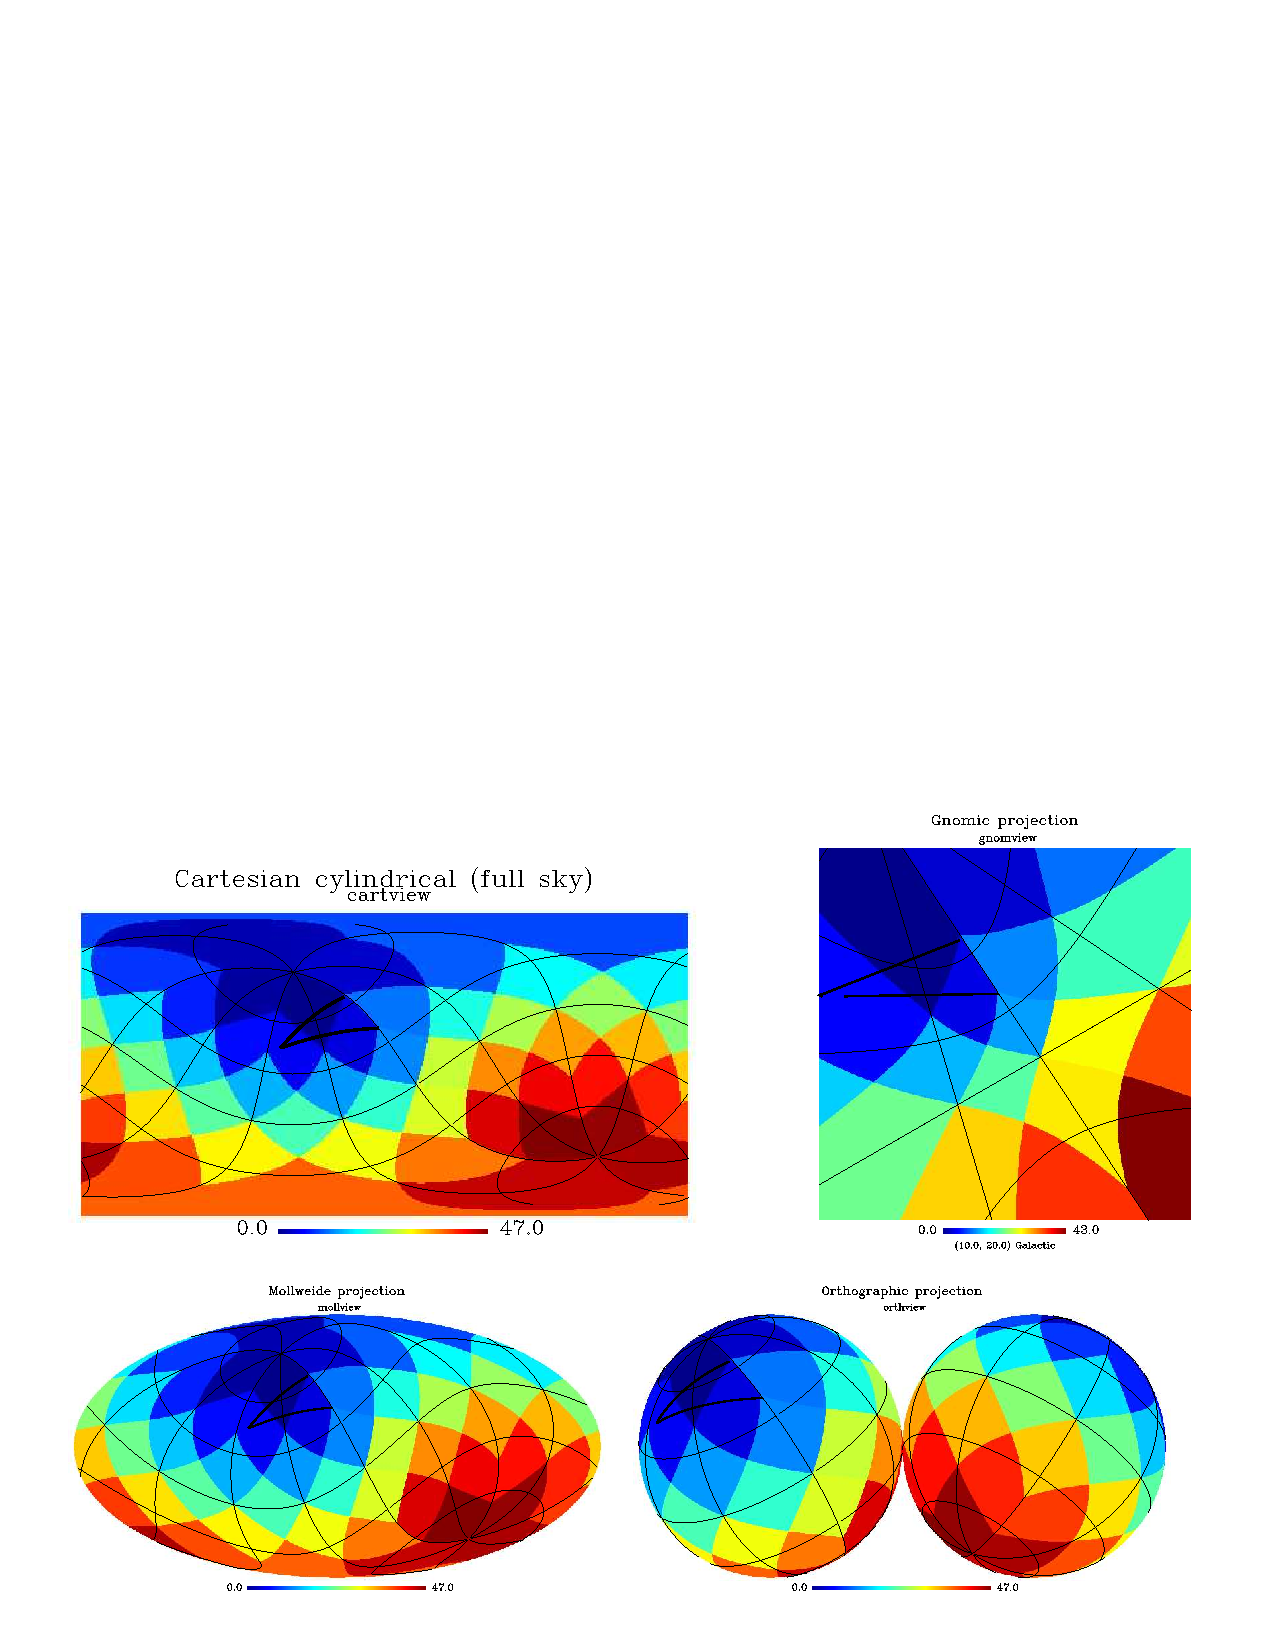
\includegraphics[bb=0pt 0pt 550pt 374pt, width=\textwidth,clip]{fig/merge_visu}}
}{%for html
%\centerline{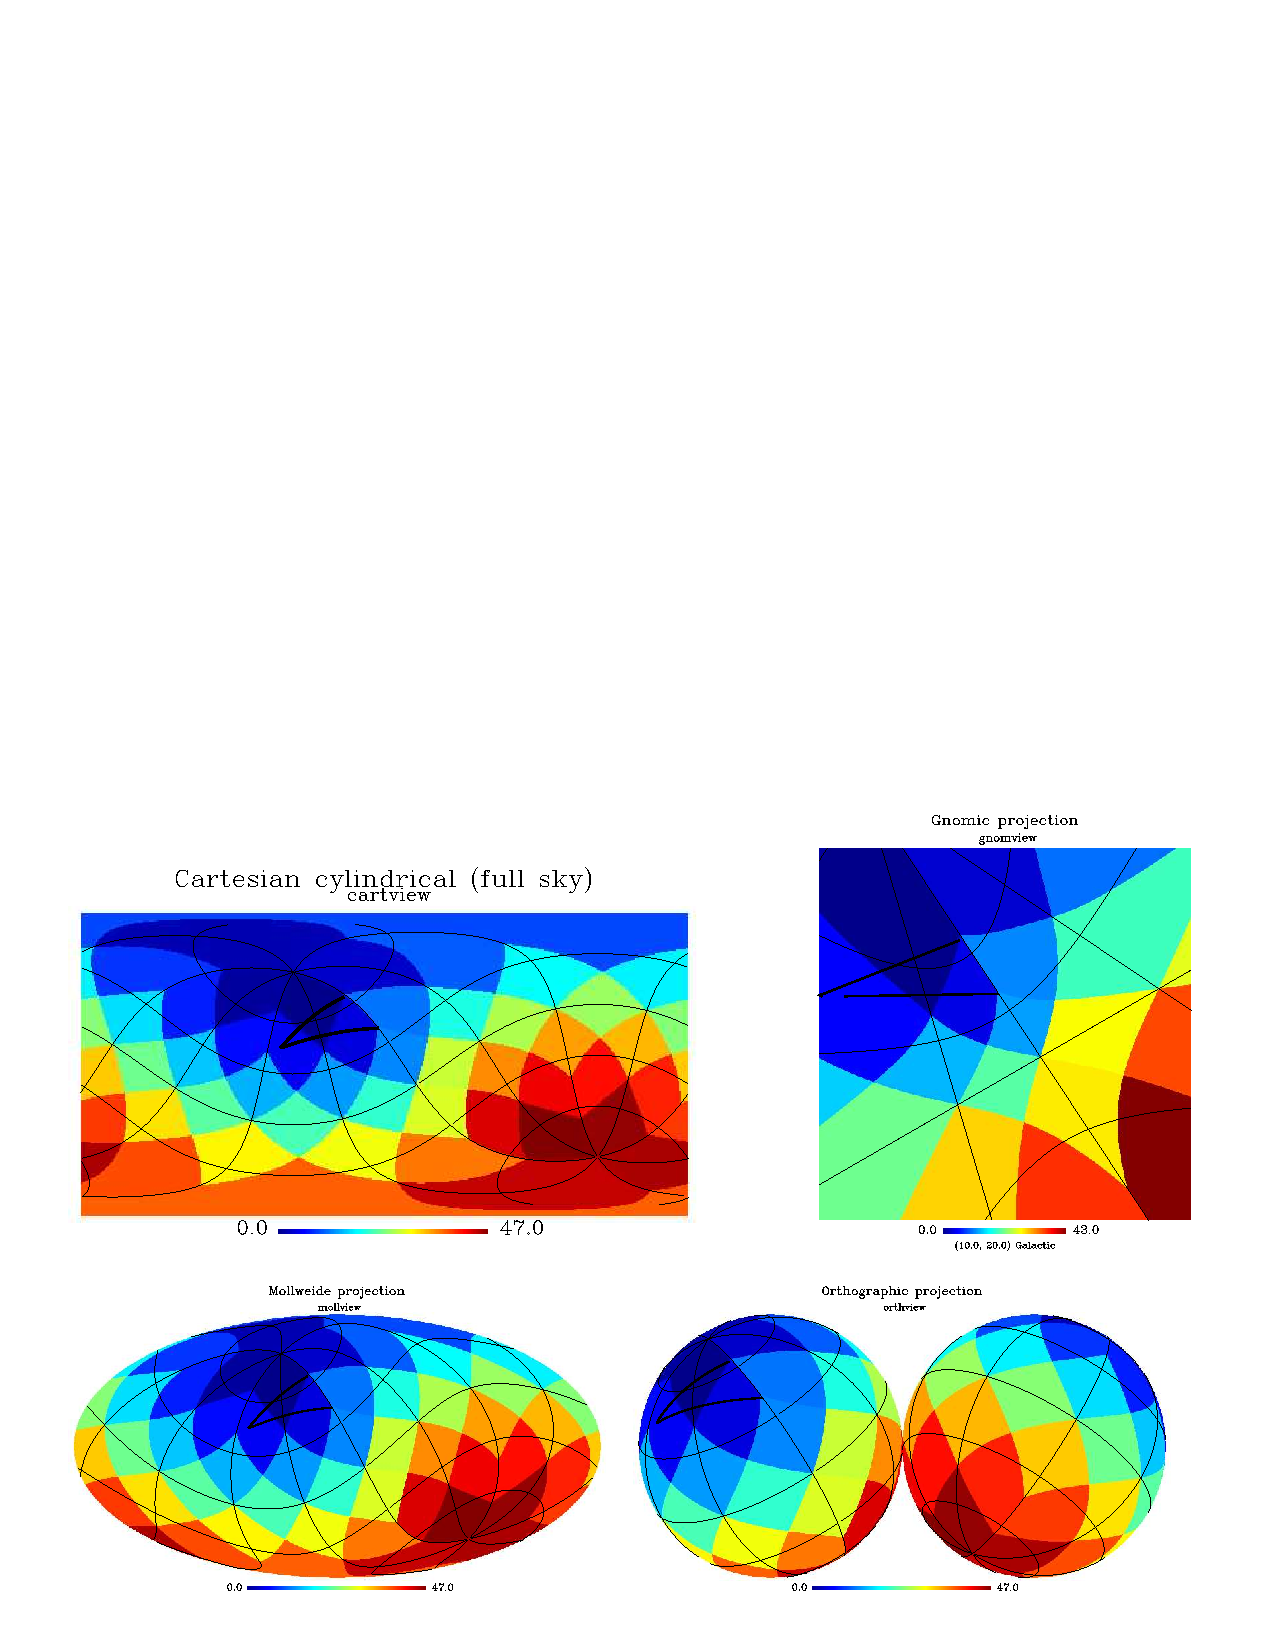
\includegraphics[bb=1pt 1pt 600pt 800pt, width=5in]{fig/merge_visu}\myhtmlimage{}}
%%%\centerline{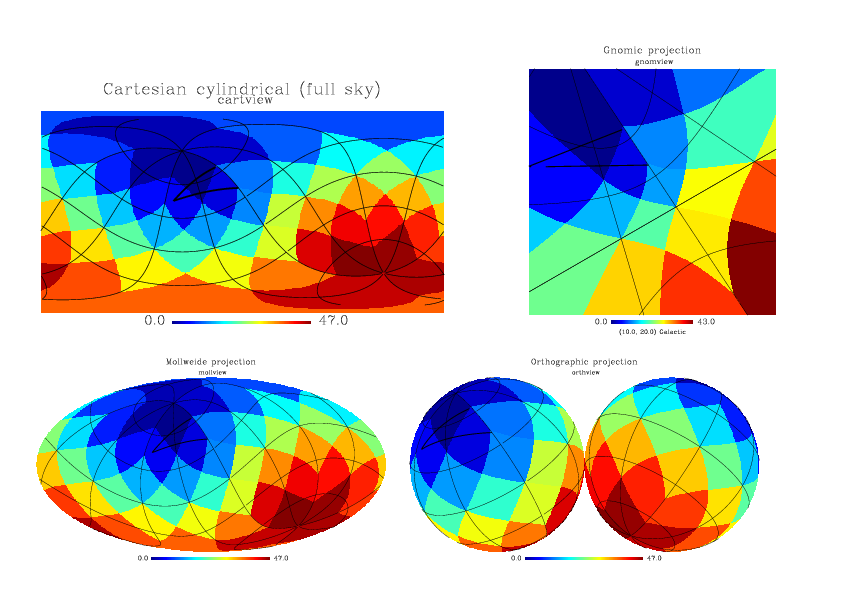
\includegraphics[width=0.5\textwidth]{fig/merge_visu_large}{}}
\centerline{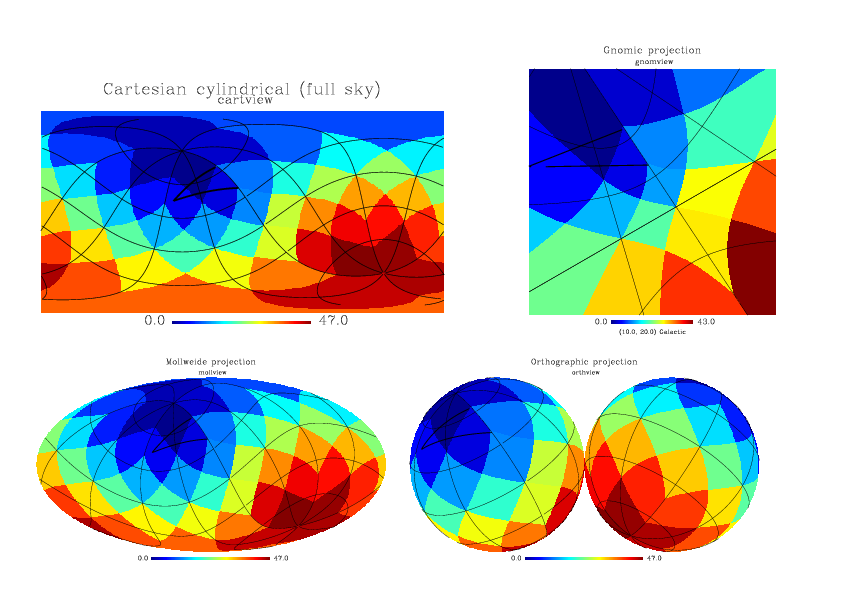
\includegraphics[width=520pt]{fig/merge_visu_large}{}}%rescaled for JPL web site -> ~720
}
\caption{%
\label{page:plot_visu}%
\label{fig:plot_visu}%
Figures produced by \htmlref{cartview}{idl:cartview},
\htmlref{gnomview}{idl:gnomview}, \htmlref{mollview}{idl:mollview} and \htmlref{orthview}{idl:orthview}, see respective
routine documentation for details.}
\end{figure}
%--------

%-------------------------------------------
\begin{examples}
{3}
{
\begin{tabular}{l} %%%% use this tabular format %%%%

map  = findgen(48) \\
mycommand = 'x=findgen(64)/10. \& ' + \$ \\
$\quad\quad$	'plot,x,sin(x),pos=[0.8,0.8,0.99,0.99],/noerase \&' +\$ \\
$\quad\quad$	'xyouts,0.5,0.5,''Hello World !'',/normal,charsize=2,align=0.5'  \\
\htmlref{\thedocid}{idl:mollview},map, \mylink{idl:mollview:execute}{execute}=mycommand, \mylink{idl:mollview:png}{png}='plot\_example\_execute.png',\mylink{idl:mollview:preview}{/preview},\$ \\
$\quad\quad$	\mylink{idl:mollview:graticule}{/graticule},\mylink{idl:mollview:glsize}{/glsize} \\
\end{tabular}
}
{produces a PNG file containing a Mollweide projection of a pixel index map
with labeled graticules, a simple sine wave in the
upper right corner, and some greetings, as shown on Figure~\ref{fig:plot_example_execute} on page~\pageref{page:plot_example_execute}
}
\end{examples}
%-------
\begin{figure}[h!]
\latexhtml{%for latex
\centerline{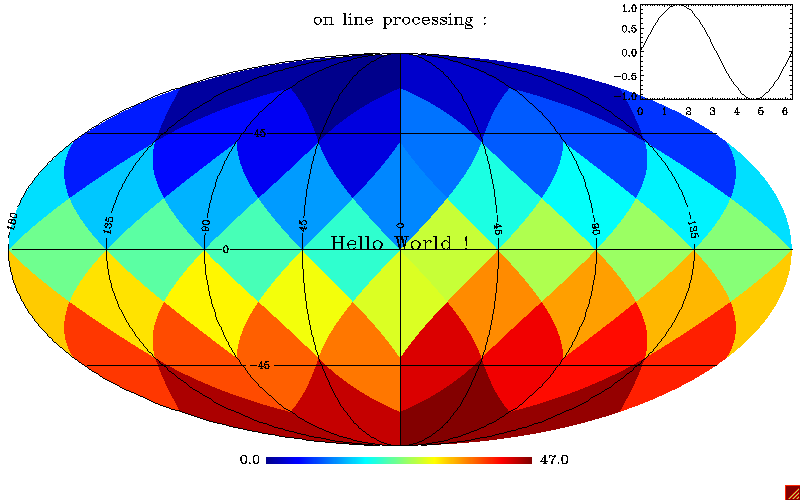
\includegraphics[bb=0pt 20pt 800pt 500pt, width=0.7\textwidth,clip]{fig/plot_example_execute}}
}{%for html
%%%\centerline{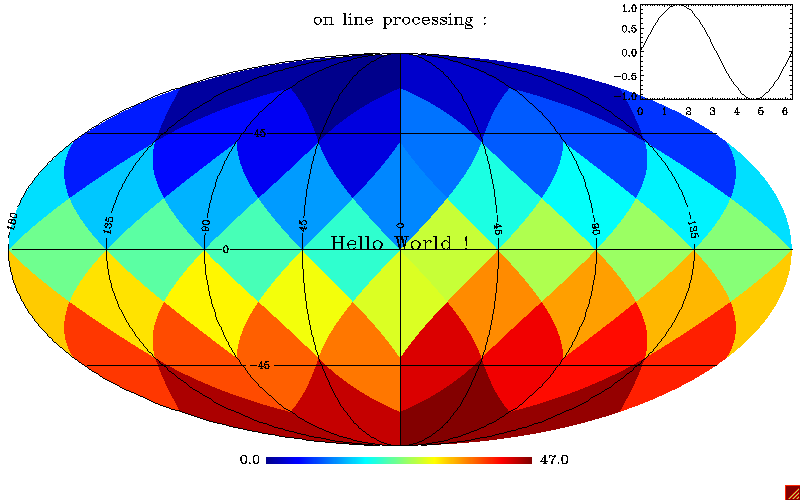
\includegraphics[width=0.5\textwidth]{fig/plot_example_execute}{}}
\centerline{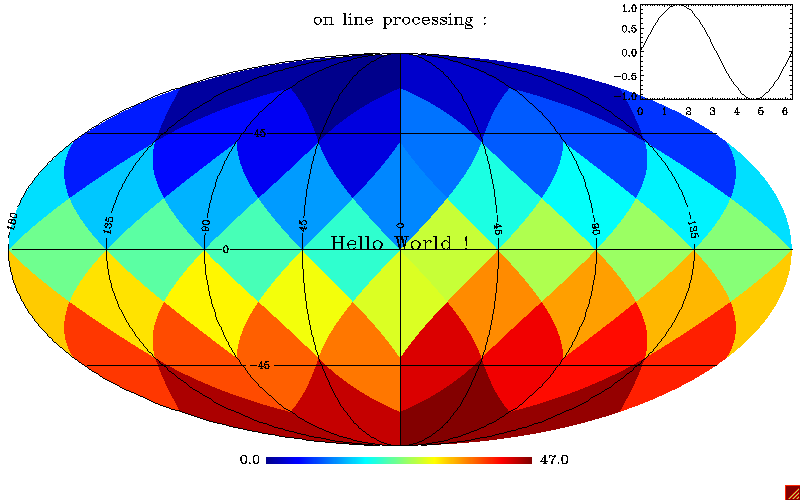
\includegraphics[width=520pt]{fig/plot_example_execute}{}}%rescaled for JPL web site -> ~720
}
\caption{%
\label{page:plot_example_execute}%
\label{fig:plot_example_execute}%
Figure produced by example \#3.}
\end{figure}
%-------



%-------------------------------------------
\label{page:example_hires_cutsky}
\begin{examples}
{4}
{
\begin{tabular}{l} %%%% use this tabular format %%%%

pixel  = l64indgen(400000) \\
signal = pixel * 10.0 \\
file = 'cutsky.fits' \\
\htmlref{write\_fits\_cut4}{idl:write_fits_cut4}, file, pixel+100000, signal, nside=32768, /ring \\
\htmlref{gnomview}{idl:gnomview}, \mylink{idl:mollview:file}{file}, \mylink{idl:mollview:graticule}{rot}=[0,90], \mylink{idl:mollview:graticule}{grat}=30, \mylink{idl:mollview:titleplot}{title}='high res. cut-sky map' \\
\end{tabular}
}
{produces and plots a high resolution map (6.4 arcsec/pixel), in which only a very small subset of
pixels is observed}
\end{examples}
%-------------------------------------------
\begin{examples}
{5}
{
\begin{tabular}{l} %%%% use this tabular format %%%%

file = 'wmap\_band\_iqumap\_r9\_5yr\_K\_v3.fits' \\
\htmlref{\thedocid}{idl:mollview}, \mylink{idl:mollview:file}{file}, \mylink{idl:mollview:titleplot}{title}='Linear Color Scale', \mylink{idl:mollview:silent}{/silent} \\
\thedocid, file,\mylink{idl:mollview:asinh}{/asinh},title='Sinh!u-1!n Color Scale' , /silent \\
\thedocid, file,\mylink{idl:mollview:hist_equal}{/hist}, title='Histogram Equalized Color Scale', /silent \\
\thedocid, file,\mylink{idl:mollview:log}{/log},  title='Log Scale', /silent \\
\end{tabular}
}
{produces Mollweide projections of the same map (here the WMAP-5yr K band) with
various color scales: linear, Inverse
Hyperbolic Sine, Histogram Equalized, and Log. See Figure~\ref{fig:merge_wmapKband} on page~\pageref{page:merge_wmapKband}
}
\end{examples}
%
\begin{figure}[h!]
\latexhtml{%for latex
%\centerline{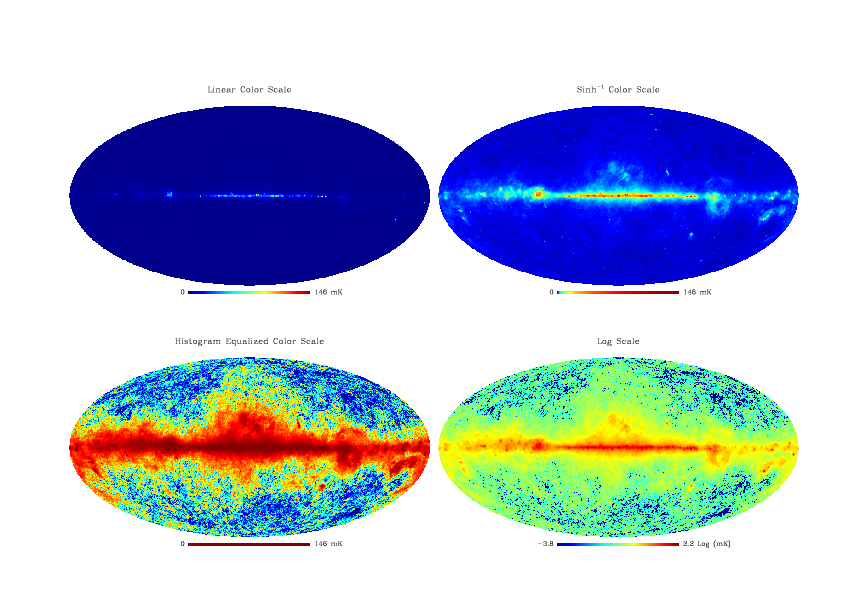
\includegraphics[bb=0pt 0pt 842pt 595pt, width=0.99\textwidth,clip]{fig/merge_wmapKband}}
\centerline{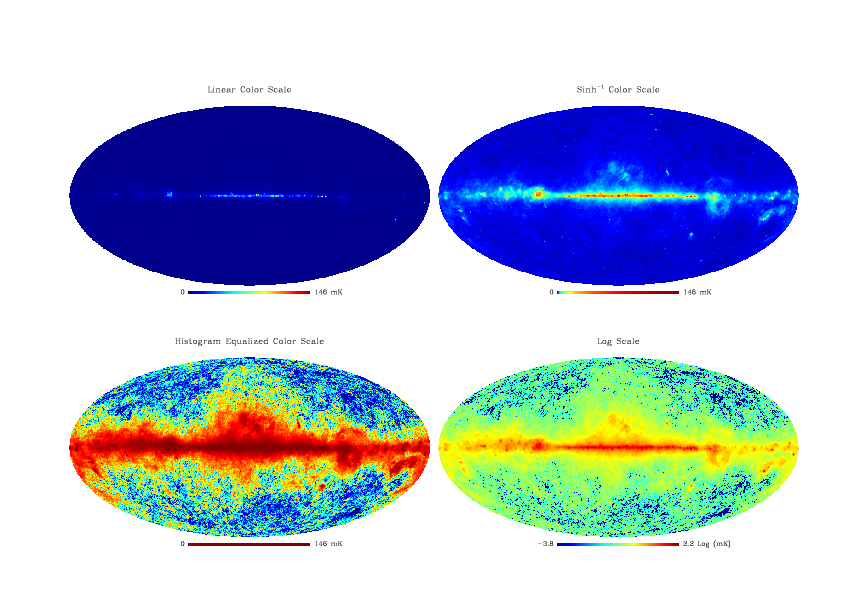
\includegraphics[bb=30pt 40pt 812pt 510pt, width=0.99\textwidth,clip]{fig/merge_wmapKband}}
}{%for html
%%%\centerline{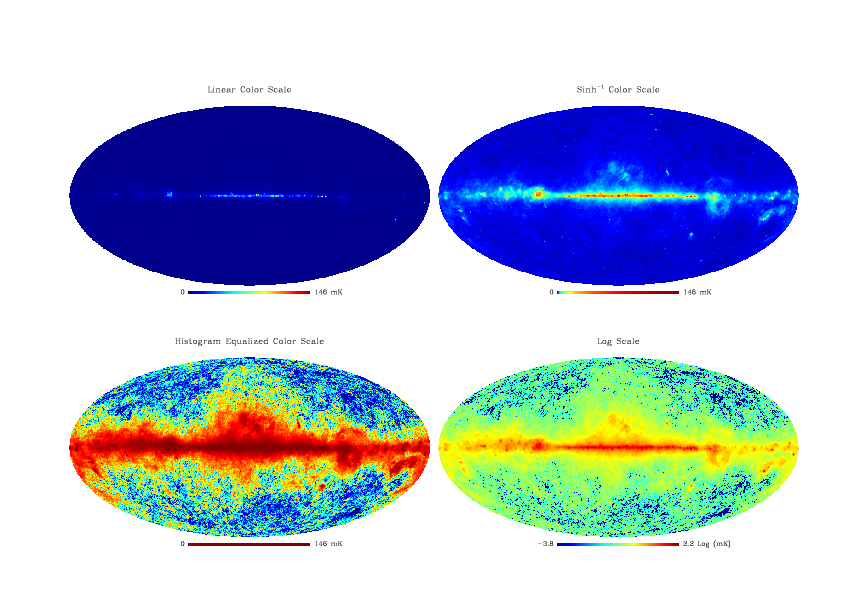
\includegraphics[width=0.5\textwidth]{fig/merge_wmapKband}{}}
\centerline{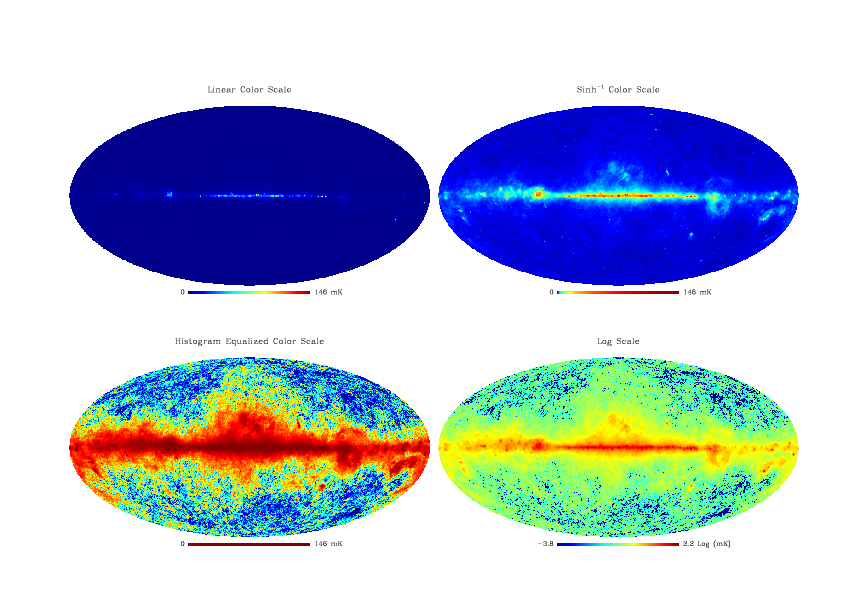
\includegraphics[width=520pt]{fig/merge_wmapKband}{}}%rescaled for JPL web site -> ~720
}
\caption{%
\label{page:merge_wmapKband}%
\label{fig:merge_wmapKband}%
Illustration (generated by example~\#5) of the various color scales available.}
\end{figure}

%-------------------------------------------
\begin{examples}
{1}
{
\begin{tabular}{l} %%%% use this tabular format %%%%
\htmlref{\thedocid}{idl:mollview},  \mylink{idl:mollview:file}{'planck100GHZ-LFI.fits'}, \mylink{idl:mollview:min}{min}=-100, \mylink{idl:mollview:max}{max}=100, \mylink{idl:mollview:graticule}{/graticule}, \$ \\
$\quad$	 \mylink{idl:mollview:titleplot}{title}='Simulated Planck LFI Sky Map at 100GHz'\\
\end{tabular}
}
{\thedocid \ reads in the map 'planck100GHZ-LFI.fits' and generates
an output image in which
the temperature scale has been set to lie between $\pm$ 100 ($\mu$K),
a \mylink{idl:mollview:graticule}{graticule} with a 45 degree step in longitude and latitude is drawn,
and the \mylink{idl:mollview:titleplot}{title} 'Simulated Planck LFI Sky Map at 100GHz' appended to the image.
}
\end{examples}


% -*- LaTeX -*-


\renewcommand{\facname}{{neighbours\_nest }}

\sloppy


\title{\healpix IDL Facility User Guidelines}
\docid{neighbours\_nest} \section[neighbours\_nest]{ }
\label{idl:neighbours_nest}
\docrv{Version 1.0}
\author{Eric Hivon}
\abstract{This document describes the \healpix IDL facility \facname.}


\begin{facility}
{This IDL facility returns the number and indices of the topological immediate neighbours 
of a central pixel. The pixels
are ordered in a clockwise sense (when watching the sphere from the outside) 
about the central pixel with the
southernmost pixel in first element. For the four pixels in the southern 
corners of the
equatorial faces which have two equally southern neighbours the
routine returns the southwestern pixel first and proceeds clockwise.}
{src/idl/toolkit/neighbours\_nest.pro}
\end{facility}

\begin{IDLformat}
{\facname(Nside, Ipix0, Listpix [,Nneigh])}
\end{IDLformat}

\begin{qualifiers}
  \begin{qulist}{} %%%% NOTE the ``extra'' brace here %%%%
    \item[Nside] \healpix resolution parameter (scalar integer),
         should be a valid Nside (power of 2)
    \item[Ipix0] NESTED-scheme index of central pixel in [0,12*Nside$^2$-1]
    \item[Listpix] output: list of neighbouring pixel (NESTED scheme index) of
size {\tt Nneigh}
    \item[Nneigh] optional output: number of neighbours of pixel {\tt \#Ipix0}. 
   Usually 8, sometimes 7 (for 8 particular pixels) or 6 (if Nside=1)
  \end{qulist}
\end{qualifiers}

% \begin{keywords}
%   \begin{kwlist}{} %%% extra brace
%     \item[] 
%   \end{kwlist}
% \end{keywords}  

\begin{codedescription}
{\facname calls {\tt pix2xy\_nest} to find location of central pixel within the pixelation
base-face, and then {\tt xy2pix\_nest} to find neighbouring pixels within the same
face, or one of the bit manipulation routines if the neighbouring pixel
is on a different base-face.}
\end{codedescription}



\begin{related}
  \begin{sulist}{} %%%% NOTE the ``extra'' brace here %%%%
    \item[idl] version \idlversion or more is necessary to run \facname.
    \item[\htmlref{neighbours\_ring}{idl:neighbours_ring}] returns topological immediate
neighbouring pixels of a given central pixel, using RING indexing.
    \item[\htmlref{query\_disc}{idl:query_disc}, 
          \htmlref{query\_polygon}{idl:query_polygon},]
    \item[\htmlref{query\_strip}{idl:query_strip}, \htmlref{query\_triangle}{idl:query_triangle}] render the list of pixels enclosed
  respectively in a given disc, polygon, latitude strip and triangle
    \item[\htmlref{nest2ring}{idl:pix_tools}, \htmlref{ring2nest}{idl:pix_tools}] conversion between NESTED and RING indices
  \end{sulist}
\end{related}

\begin{example}
{
\begin{tabular}{ll} %%%% use this tabular format %%%%
\facname, 4, 1, list, nneigh \\
print,nneigh,list\\
\end{tabular}
}
{
will return:8 \hskip 1cm    90 0  2  3  6  4 94 91,
listing the NESTED-indexed 8 neighbors of pixel \#1 for Nside=4
}
\end{example}


% -*- LaTeX -*-


\renewcommand{\facname}{{neighbours\_ring }}

\sloppy


\title{\healpix IDL Facility User Guidelines}
\docid{neighbours\_ring} \section[neighbours\_ring]{ }
\label{idl:neighbours_ring}
\docrv{Version 1.0}
\author{Eric Hivon}
\abstract{This document describes the \healpix IDL facility \facname.}


\begin{facility}
{This IDL facility returns the number and indices of the topological immediate neighbours 
of a central pixel. The pixels
are ordered in a clockwise sense (when watching the sphere from the outside) 
about the central pixel with the
southernmost pixel in first element. For the four pixels in the southern 
corners of the
equatorial faces which have two equally southern neighbours the
routine returns the southwestern pixel first and proceeds clockwise.}
{src/idl/toolkit/neighbours\_ring.pro}
\end{facility}

\begin{IDLformat}
{\facname(Nside, Ipix0, Listpix [,Nneigh])}
\end{IDLformat}

\begin{qualifiers}
  \begin{qulist}{} %%%% NOTE the ``extra'' brace here %%%%
    \item[Nside] \healpix resolution parameter (scalar integer),
         should be a valid Nside (power of 2)
    \item[Ipix0] RING-scheme index of central pixel in [0,12*Nside$^2$-1]
    \item[Listpix] output: list of neighbouring pixel (RING scheme index) of
size {\tt Nneigh}
    \item[Nneigh] optional output: number of neighbours of pixel {\tt \#Ipix0}. 
   Usually 8, sometimes 7 (for 8 particular pixels) or 6 (if Nside=1)
  \end{qulist}
\end{qualifiers}

% \begin{keywords}
%   \begin{kwlist}{} %%% extra brace
%     \item[] 
%   \end{kwlist}
% \end{keywords}  

\begin{codedescription}
{\facname calls ring2nest, neighbours\_nest and nest2ring}
\end{codedescription}



\begin{related}
  \begin{sulist}{} %%%% NOTE the ``extra'' brace here %%%%
    \item[idl] version \idlversion or more is necessary to run \facname.
    \item[\htmlref{neighbours\_nest}{idl:neighbours_nest}] returns topological immediate
neighbouring pixels of a given central pixel, using NESTED indexing.
    \item[\htmlref{query\_disc}{idl:query_disc}, 
          \htmlref{query\_polygon}{idl:query_polygon},]
    \item[\htmlref{query\_strip}{idl:query_strip}, \htmlref{query\_triangle}{idl:query_triangle}] render the list of pixels enclosed
  respectively in a given disc, polygon, latitude strip and triangle
    \item[\htmlref{nest2ring}{idl:pix_tools}, \htmlref{ring2nest}{idl:pix_tools}] conversion between NESTED and RING indices
  \end{sulist}
\end{related}

\begin{example}
{
\begin{tabular}{ll} %%%% use this tabular format %%%%
\facname, 4, 1, list, nneigh \\
print,nneigh,list\\
\end{tabular}
}
{
will return:8 \hskip 1cm    16  6  5  0  3  2  8  7
listing the RING-indexed 8 neighbors of pixel \#1 for Nside=4
}
\end{example}


% -*- LaTeX -*-


\renewcommand{\facname}{{npix2nside }}
\renewcommand{\FACNAME}{{NPIX2NSIDE }}

\sloppy



\title{\healpix IDL Facility User Guidelines}
\docid{\facname} \section[\facname]{ }
\label{idl:npix2nside}
\docrv{Version 1.0}
\author{Eric Hivon}
\abstract{This document describes the \healpix IDL facility \facname.}




\begin{facility}
{This IDL facility provides the \healpix resolution parameter Nside corresponding to Npix
pixels over the full sky.
}
{src/idl/toolkit/npix2nside.pro}
\end{facility}

\begin{IDLformat}
{\mylink{idl:npix2nside:Nside}{Nside=}%
\FACNAME(\mylink{idl:npix2nside:Npix}{Npix}%
 [,\mylink{idl:npix2nside:ERROR}{ERROR=}%
])}
\end{IDLformat}

\begin{qualifiers}
  \begin{qulist}{} %%%% NOTE the ``extra'' brace here %%%%
    \item[Npix\mytarget{idl:npix2nside:Npix}%
] number of pixels over the full sky (scalar integer),
         should be a valid Npix 
	($N_{\rm pix} = 12N_{\rm side}^2$ with $N_{\rm side}$ power of 2 in $\{1,\ldots,2^{29}\}$)
    \item[Nside\mytarget{idl:npix2nside:Nside}%
] on output: resolution parameter if Npix is valid, -1 otherwise
  \end{qulist}
\end{qualifiers}

\begin{keywords}
  \begin{kwlist}{} %%% extra brace
    \item[ERROR\mytarget{idl:npix2nside:ERROR}%
 =] error flag, set to 1 on output if Npix is NOT valid, or
    stays to 0 otherwise.
  \end{kwlist}
\end{keywords}  

\begin{codedescription}
{\facname checks that the given Npix is valid 
($N_{\rm pix} = 12N_{\rm side}^2$ with $N_{\rm side}$ a power of 2 in
$\{1,\ldots,2^{29}\}$) and then computes the
corresponding resolution parameter $N_{\rm side}$.}
\end{codedescription}



\begin{related}
  \begin{sulist}{} %%%% NOTE the ``extra'' brace here %%%%
    \item[idl] version \idlversion or more is necessary to run \facname.	
    \item[\htmlref{nside2npix}{idl:nside2npix}] computes Npix corresponding to Nside 
    \item[\htmlref{pix2xxx}{idl:pix_tools}, \htmlref{ang2xxx}{idl:pix_tools}, \htmlref{vec2xxx}{idl:pix_tools}, ... ] conversion between vector or angles and pixel index and vice-versa
    \item[\htmlref{vec2pix}{idl:pix_tools}, \htmlref{pix2vec}{idl:pix_tools}] conversion between vector and pixel index
    \item[\htmlref{nest2ring}{idl:pix_tools}, \htmlref{ring2nest}{idl:pix_tools}] conversion between NESTED and RING indices
  \end{sulist}
\end{related}

\begin{example}
{
\begin{tabular}{ll} %%%% use this tabular format %%%%
Nside = npix2nside(49152, ERROR=error)
\end{tabular}
}
{
Nside will be 64 because 49152 is a valid pixel number (=12*64$^2$ and 64 is a power of 2), and error will be 0}
\end{example}
\begin{example}
{
\begin{tabular}{ll} %%%% use this tabular format %%%%
Nside = npix2nside(49151, ERROR=error)
\end{tabular}
}
{
Nside will be -1 and error: 1, because 49151 is not a valid number of \healpix
pixels over the full sky.}
\end{example}



% -*- LaTeX -*-


\renewcommand{\facname}{{nside2npix }}
\renewcommand{\FACNAME}{{NSIDE2NPIX }}

\sloppy



\title{\healpix IDL Facility User Guidelines}
\docid{nside2npix} \section[nside2npix]{ }
\label{idl:nside2npix}
\docrv{Version 1.0}
\author{Eric Hivon}
\abstract{This document describes the \healpix IDL facility \facname.}




\begin{facility}
{This IDL facility provides the number of pixels Npix over the full sky corresponding
to resolution parameter Nside.
}
{src/idl/toolkit/nside2npix.pro}
\end{facility}

\begin{IDLformat}
{Npix=\FACNAME(Nside [,ERROR=])}
\end{IDLformat}

\begin{qualifiers}
  \begin{qulist}{} %%%% NOTE the ``extra'' brace here %%%%
    \item[Nside] \healpix resolution parameter (scalar integer),
         should be a valid Nside (power of 2 $ \le 2^{29}$)
    \item[Npix] number of pixels, Npix = 12*Nside$^2$ if Nside is a valid
    resolution parameter or -1 otherwise
  \end{qulist}
\end{qualifiers}

\begin{keywords}
  \begin{kwlist}{} %%% extra brace
    \item[ERROR =] error flag, set to 1 on output if Nside is NOT valid, or
    stays to 0 otherwise.
  \end{kwlist}
\end{keywords}  

\begin{codedescription}
{\facname checks that the given Nside is valid (power of 2 in
$\{1,\ldots,2^{29}\}$) and then computes the
corresponding number of pixels $N_{\rm pix} = 12N_{\rm side}^2$.}
\end{codedescription}



\begin{related}
  \begin{sulist}{} %%%% NOTE the ``extra'' brace here %%%%
    \item[idl] version \idlversion or more is necessary to run \facname.	
    \item[\htmlref{npix2nside}{idl:npix2nside}] computes Nside corresponding to Npix
    \item[\htmlref{pix2xxx}{idl:pix_tools}, \htmlref{ang2xxx}{idl:pix_tools}, \htmlref{vec2xxx}{idl:pix_tools}, ... ] conversion between vector or angles and pixel index and vice-versa
    \item[\htmlref{vec2pix}{idl:pix_tools}, \htmlref{pix2vec}{idl:pix_tools}] conversion between vector and pixel index
    \item[\htmlref{nest2ring}{idl:pix_tools}, \htmlref{ring2nest}{idl:pix_tools}] conversion between NESTED and RING indices
  \end{sulist}
\end{related}

\begin{example}
{
\begin{tabular}{ll} %%%% use this tabular format %%%%
Npix = nside2npix(256, ERROR=error)
\end{tabular}
}
{
Npix will be 786432 the number of pixels over the full sky for the \healpix
resolution parameter 256 and error will be 0}
\end{example}
\begin{example}
{
\begin{tabular}{ll} %%%% use this tabular format %%%%
Npix = nside2npix(248, ERROR=error)
\end{tabular}
}
{
Npix will be -1 and error: 1, because 248 is not a valid value for a \healpix
resolution parameter}
\end{example}



% -*- LaTeX -*-


\renewcommand{\facname}{{nside2ntemplates }}
\renewcommand{\FACNAME}{{NSIDE2NTEMPLATES }}

\sloppy



\title{\healpix IDL Facility User Guidelines}
\docid{nside2ntemplates} \section[nside2ntemplates]{ }
\label{idl:nside2ntemplates}
\docrv{Version 1.0}
\author{Eric Hivon}
\abstract{This document describes the \healpix IDL facility \facname.}


\begin{facility}
{This IDL facility provides the number of template pixels Ntemplates corresponding
to resolution parameter Nside. Each template pixel has a different shape that
{\em can not} be matched (by rotation or reflexion) to that of any of the other templates.
}
{src/idl/toolkit/nside2ntemplates.pro}
\end{facility}

\begin{IDLformat}
{\mylink{idl:nside2ntemplates:Ntemplates}{Ntemplates=}%
\FACNAME(\mylink{idl:nside2ntemplates:Nside}{Nside}%
 [,\mylink{idl:nside2ntemplates:ERROR}{ERROR=}%
])}
\end{IDLformat}

\begin{qualifiers}
  \begin{qulist}{} %%%% NOTE the ``extra'' brace here %%%%
    \item[Nside\mytarget{idl:nside2ntemplates:Nside}%
] \healpix resolution parameter (scalar integer),
         should be a valid Nside (power of 2 in $\{1,\ldots,2^{29}\}$)
    \item[Ntemplates\mytarget{idl:nside2ntemplates:Ntemplates}%
] number of templates
  \end{qulist}
\end{qualifiers}

\begin{keywords}
  \begin{kwlist}{} %%% extra brace
    \item[ERROR\mytarget{idl:nside2ntemplates:ERROR}%
 =] error flag, set to 1 on output if Nside is NOT valid, or
    stays to 0 otherwise.
  \end{kwlist}
\end{keywords}  

\begin{codedescription}
{\facname outputs the number of template pixels
  $$\ntemplate=\frac{1+\nside(\nside+6)}{4}.$$ If the argument $\nside$ is not
  valid, a  warning is issued and the error flag is raised.}
\end{codedescription}



\begin{related}
  \begin{sulist}{} %%%% NOTE the ``extra'' brace here %%%%
    \item[idl] version \idlversion or more is necessary to run \facname.	
  \item[\htmlref{template\_pixel\_ring}{idl:template_pixel_xxx}]
  \item[\htmlref{template\_pixel\_nest}{idl:template_pixel_xxx}] return the
  template pixel associated with any \healpix pixel
  \item[\htmlref{same\_shape\_pixels\_ring}{idl:same_shape_pixels_xxx}] 
  \item[\htmlref{same\_shape\_pixels\_nest}{idl:same_shape_pixels_xxx}] 
  return
  the ordered list of pixels having the same shape as a given pixel template
  \end{sulist}
\end{related}

\begin{example}
{
\begin{tabular}{ll} %%%% use this tabular format %%%%
Ntemplates = nside2ntemplates(256, ERROR=error)
\end{tabular}
}
{
Ntemplates will be 16768 the number of template pixels for the \healpix
resolution parameter 256 and error will be 0}
\end{example}


% -*- LaTeX -*-

% PLEASE USE THIS FILE AS A TEMPLATE FOR THE DOCUMENTATION OF YOUR OWN
% FACILITIES: IN PARTICULAR, IT IS IMPORTANT TO NOTE COMMENTS MADE IN
% THE TEXT AND TO FOLLOW THIS ORDERING. THE FORMAT FOLLOWS ONE USED BY
% THE COBE-DMR PROJECT.	
% A.J. Banday, April 1999.




\sloppy



\title{\healpix IDL Facility User Guidelines}
\docid{orthcursor} \section[orthcursor]{ }
\label{idl:\thedocid}
\docrv{Version 1.2}
\author{Eric Hivon}
\abstract{This document describes the \healpix facility orthcursor.}


\begin{facility}
{This IDL facility provides a point-and-click interface for finding
the astronomical location, value and pixel index of the pixels nearest 
to the pointed position on a orthographic projection of a \healpix map.}
{src/idl/visu/orthcursor.pro}
\end{facility}

\begin{IDLformat}
{ORTHCURSOR, [cursor\_type=, file\_out=]}
\end{IDLformat}

\begin{qualifiers}
\hbox{\hspace{5cm}		see \htmlref{mollcursor}{idl:mollcursor}}
\end{qualifiers}

\begin{codedescription}
{orthcursor should be called immediately after orthview. It gives the longitude,
latitude, map value and pixel number
corresponding to the cursor position in the window containing the map generated
by orthview. For more details, or in case
of problems under {\bf Mac OS X}, see \htmlref{mollcursor}{idl:mollcursor}.}
\end{codedescription}



\begin{related}
\hbox{\hspace{5cm}	see \htmlref{mollcursor}{idl:mollcursor}}
\end{related}


\begin{example}
{
\begin{tabular}{ll} %%%% use this tabular format %%%%
orthcursor & \ 
\end{tabular}
}
{After orthview has read in a map and generated
its orthographic projection, orthcursor is run to determine the
position and flux of bright synchrotron sources, for example.}
\end{example}



% -*- LaTeX -*-

% PLEASE USE THIS FILE AS A TEMPLATE FOR THE DOCUMENTATION OF YOUR OWN
% FACILITIES: IN PARTICULAR, IT IS IMPORTANT TO NOTE COMMENTS MADE IN
% THE TEXT AND TO FOLLOW THIS ORDERING. THE FORMAT FOLLOWS ONE USED BY
% THE COBE-DMR PROJECT.	
% A.J. Banday, April 1999.




\sloppy



\title{\healpix IDL Facility User Guidelines}
\docid{orthview} \section[orthview]{ }
\label{idl:\thedocid}
\docrv{Version 1.2}
\author{Eric Hivon}
\abstract{This document describes the \healpix facility orthview.}



\begin{facility}
{This IDL facility provides a means to visualise a full sky or half sky orthographic projection 
(projection onto a tangent plane from a point located at infinity) of
\healpix and COBE Quad-Cube maps in an IDL environment. 
It also offers the possibility to
generate GIF, JPEG, PDF, PNG and Postscript color-coded images of the projected map.
The projected (but not color-coded) data can also be output in FITS files and
IDL arrays.}
{src/idl/visu/orthview.pro}
\end{facility}

\begin{IDLformat}
{ORTHVIEW, 
\normalsize{
\mylink{idl:mollview:file}{File}, 
[ \mylink{idl:mollview:select}{Select}, ]
[ \mylink{idl:mollview:asinh}{/ASINH}, 
\mylink{idl:mollview:charsize}{CHARSIZE=}, 
\mylink{idl:mollview:charsize}{CHARTHICK=}, 
\mylink{idl:mollview:colt}{COLT=}, 
\mylink{idl:mollview:coord}{COORD=}, 
\mylink{idl:mollview:crop}{/CROP}, 
\mylink{idl:mollview:execute}{EXECUTE=}, 
\mylink{idl:mollview:factor}{FACTOR=}, 
\mylink{idl:mollview:fits}{FITS=}, 
\mylink{idl:mollview:flip}{/FLIP}, 
\mylink{idl:mollview:gal_cut}{GAL\_CUT=}, 
\mylink{idl:mollview:gif}{GIF=}, 
\mylink{idl:mollview:glsize}{GLSIZE=}, 
\mylink{idl:mollview:graticule}{GRATICULE=}, 
\mylink{idl:mollview:half_sky}{/HALF\_SKY}, 
\mylink{idl:mollview:hbound}{HBOUND=}, 
\mylink{idl:mollview:help}{/HELP}, 
\mylink{idl:mollview:hist_equal}{/HIST\_EQUAL}, 
\mylink{idl:mollview:hxsize}{HXSIZE=}, 
\mylink{idl:mollview:iglsize}{IGLSIZE=}, 
\mylink{idl:mollview:igraticule}{IGRATICULE=}, 
\mylink{idl:mollview:log}{/LOG}, 
\mylink{idl:mollview:map_out}{MAP\_OUT=}, 
\mylink{idl:mollview:max}{MAX=}, 
\mylink{idl:mollview:min}{MIN=}, 
\mylink{idl:mollview:nested}{/NESTED}, 
\mylink{idl:mollview:no_dipole}{/NO\_DIPOLE}, 
\mylink{idl:mollview:no_monopole}{/NO\_MONOPOLE}, 
\mylink{idl:mollview:nobar}{/NOBAR}, 
\mylink{idl:mollview:nolabels}{/NOLABELS}, 
\mylink{idl:mollview:noposition}{/NOPOSITION}, 
\mylink{idl:mollview:offset}{OFFSET=}, 
\mylink{idl:mollview:outline}{OUTLINE=}, 
\mylink{idl:mollview:png}{PNG=}, 
\mylink{idl:mollview:polarization}{POLARIZATION=}, 
\mylink{idl:mollview:preview}{/PREVIEW}, 
\mylink{idl:mollview:ps}{PS=}, 
\mylink{idl:mollview:pxsize}{PXSIZE=}, 
\mylink{idl:mollview:pysize}{PYSIZE=}, 
\mylink{idl:mollview:reso_arcmin}{RESO\_ARCMIN=}, 
\mylink{idl:mollview:retain}{RETAIN=}, 
\mylink{idl:mollview:rot}{ROT=}, 
\mylink{idl:mollview:save}{/SAVE}, 
\mylink{idl:mollview:shaded}{/SHADED}, 
\mylink{idl:mollview:silent}{/SILENT}, 
\mylink{idl:mollview:subtitle}{SUBTITLE=}, 
\mylink{idl:mollview:titleplot}{TITLEPLOT=}, 
\mylink{idl:mollview:transparent}{TRANSPARENT=}, 
\mylink{idl:mollview:truecolors}{TRUECOLORS=}, 
\mylink{idl:mollview:units}{UNITS=}, 
\mylink{idl:mollview:window}{WINDOW=}, 
\mylink{idl:mollview:xpos}{XPOS=}, 
\mylink{idl:mollview:ypos}{YPOS=}]
}
}
\end{IDLformat}

%\ mylink: to avoid automatic processing by make_internal_links.sh

\begin{qualifiers}
  \begin{qulist}{} %%%% NOTE the ``extra'' brace here %%%%
\item [{\  }] For a full list of qualifiers see \htmlref{mollview}{idl:mollview}
  \end{qulist}
\end{qualifiers}

\begin{keywords}
  \begin{kwlist}{} %%%% NOTE the ``extra'' brace here %%%%
\item [{\  }] For a full list of keywords see \htmlref{mollview}{idl:mollview}
  \end{kwlist}
\end{keywords}


\renewcommand{\projfullname}{{an orthographic}}
\begin{codedescription}
{
% to be included in codedesciption part of 
% cartview_idl.tex, mollview_idl.tex
% with
%\renewcommand{\projfullname}{a Mollweide}
%\begin{codedescription}
%{
% to be included in codedesciption part of 
% cartview_idl.tex, mollview_idl.tex
% with
%\renewcommand{\projfullname}{a Mollweide}
%\begin{codedescription}
%{\input{mollview_description_idl}}
%\end{codedescription}
{\thedocid{} reads in a \healpix sky map in FITS format and generates
\projfullname \ projection of it, that can be visualized on the screen or
exported in a GIF, JPEG, PNG, PDF or Postscript file. \thedocid{}  allows the selection of
the coordinate system, map size, color table, color bar inclusion,
linear, log, hybrid or histogram equalised color scaling, 
maximum and 
minimum range for the plot, plot-title {\it etc}. It also allows the representation of the
polarization field.}
}
%\end{codedescription}
{\thedocid{} reads in a \healpix sky map in FITS format and generates
\projfullname \ projection of it, that can be visualized on the screen or
exported in a GIF, JPEG, PNG, PDF or Postscript file. \thedocid{}  allows the selection of
the coordinate system, map size, color table, color bar inclusion,
linear, log, hybrid or histogram equalised color scaling, 
maximum and 
minimum range for the plot, plot-title {\it etc}. It also allows the representation of the
polarization field.}
}
\end{codedescription}

%
% defines the field 'RELATED' for mollview, gnomview, orthview,
% cartview

\begin{related}
  \begin{sulist}{} %%%% NOTE the ``extra'' brace here %%%%
  \item[idl] version \idlversion or more is necessary to run \thedocid
  \item[ghostview] ghostview or a similar facility is required to view
	  the Postscript image generated by \thedocid.
  \item[xv] xv or a similar facility is required to view the
            GIF/PNG image generated by \thedocid  (a browser can also 
            be used).
  \item[synfast] This \healpix facility will generate the FITS format 
            sky map to be input to \thedocid.
  \item[{\htmlref{cartview}{idl:cartview}}] 
	IDL facility to generate a Cartesian projection of
  	a \healpix map.
  \item[{\htmlref{cartcursor}{idl:cartcursor}}] 
	interactive cursor to be used with cartview
  \item[{\htmlref{gnomview}{idl:gnomview}}] 
	IDL facility to generate a gnomonic projection of
  	a \healpix map.
  \item[{\htmlref{gnomcursor}{idl:gnomcursor}}] 
	interactive cursor to be used with gnomview
  \item[{\htmlref{mollview}{idl:mollview}}] 
	IDL facility to generate a Mollweide projection of
  	a \healpix map.
  \item[{\htmlref{mollcursor}{idl:mollcursor}}] interactive cursor to be used with mollview
  \item[{\htmlref{orthview}{idl:orthview}}] 
	IDL facility to generate an orthographic projection of
  	a \healpix map.
  \item[{\htmlref{orthcursor}{idl:orthcursor}}] 
	interactive cursor to be used with orthview
  \end{sulist}
\end{related}

\begin{related}
  \begin{sulist}{} %%%% NOTE the ``extra'' brace here %%%%
  \item[{\ }] see \htmlref{mollview}{idl:mollview}
  \end{sulist}
\end{related}

% \begin{example}
% {
% \begin{tabular}{ll} %%%% use this tabular format %%%%
% orthview, & \lq planck100GHZ-LFI.fits', rot=[160,-30], reso\_arcmin=2., \$ \\
%           & pxsize = 500., title='Simulated Planck LFI Sky Map at 100GHz' \\
% \end{tabular}
% }
% {orthview reads in the map $\lq$ planck100GHZ-LFI.fits' and generates
% an output 500$\times$500 image, with a resolution of 2 arcmin/pixel at
% the center, in which
% the temperature scale has been set to lie between $\pm$ 100 ($\mu$K), 
% and the title $\lq$ Simulated Planck
% LFI Sky Map at 100GHz' appended to the image. The map is centered on 
% ($l=$160, $b=$-30) }
% \end{example}



\begin{example}
{
\begin{tabular}{l} %%%% use this tabular format %%%%

map  = findgen(48) \\
triangle= create\_struct('coord','G','ra',[0,80,0],'dec',[40,45,65]) \\
orthview,map,/online,graticule=[45,30],rot=[10,20,30],\$ \\
$\quad$	   title='Orthographic projection',subtitle='orthview' \$ \\
$\quad$          outline=triangle \\
\end{tabular}
}
{makes an orthographic projection of map (see Figure~\ref{fig:plot_visu}d on
page~\pageref{page:plot_visu}) after an arbitrary rotation, with a graticule grid
(with a 45$^o$ step in longitude and 30$^o$ in latitude) and an arbitrary triangular outline}
\end{example}

% -*- LaTeX -*-


\renewcommand{\facname}{{pix2xxx, ang2xxx,... }}
\renewcommand{\FACNAME}{{PIX2XXX, ANG2XXX,...}}

\sloppy



\title{\healpix IDL Facility User Guidelines}
\docid{pix2xxx,~ang2xxx, vec2xxx,~nest2ring,~ring2nest} 
\section[pix2xxx, ang2xxx, vec2xxx, nest2ring, ring2nest]{ }
\label{idl:pix_tools}
\docrv{Version 1.1}
\author{Eric Hivon} % same layout as Frode pix_tools
\abstract{This document describes the \healpix IDL facilities \facname}




\begin{facility}
{These routines provide conversion between pixel number in the \healpix map and $(\theta,\phi)$ or $(x,y,z)$ coordinates on the sphere. Some of these routines are listed here.
}
{src/idl/toolkit/}
\end{facility}

% \begin{IDLformat}
% {Npix=\FACNAME(Nside [,ERROR=])}
% \end{IDLformat}

\begin{qualifiers}
{
\begin{tabular}{p{0.15\hsize} p{0.15\hsize} p{0.1\hsize} p{0.50\hsize}} \hline  
\textbf{name (dim.)} & \textbf{type} & \textbf{in/out} & \textbf{description} \\ \hline
                   &   &   &                           \\ %%% for presentation
nside\mytarget{idl:pix_tools:nside} & scalar integer & IN & $\nside$ parameter for the \healpix map. \\
ipnest(n)\mytarget{idl:pix_tools:ipnest} & vector integer & --- & pixel identification number in NESTED scheme over the range \{0,$\npix-1$\}. \\
ipring(n)\mytarget{idl:pix_tools:ipring} & vector integer & --- & pixel identification number in RING scheme over the range \{0,$\npix-1$\}. \\
theta(n)\mytarget{idl:pix_tools:theta}  & vector double & --- & colatitude in radians measured southward from
                   north pole in \{0,$\pi$\}\\
phi(n)\mytarget{idl:pix_tools:phi} & vector double & --- & longitude in radians, measured eastward in \{0,$2\pi$\}. \\ 
vector(n,3)\mytarget{idl:pix_tools:vector} & array double & --- & three dimensional cartesian position vector
                   $(x,y,z)$. The north pole is $(0,0,1)$. An output vector is
                   normalised to unity. The coordinates are ordered as follows
                   $x(0),\ldots,x(n-1),\ y(0),\ldots,y(n-1),\ z(0),\ldots,z(n-1)$
                   \\
vertex(n,3,4)\mytarget{idl:pix_tools:vertex} & array double & optional OUT & three dimensional cartesian position vector
                   $(x,y,z)$. Contains the location of the four vertices
                   (=corners) of a
                   pixel in the order North, West, South, East. The coordinates
                   are ordered as follows
                   $x_N(0),\ldots,x_N(n-1),\ y_N(0),\ldots,y_N(n-1),\ z_N(0),\ldots,z_N(n-1)$,
                   $x_W(0),\ldots,x_W(n-1),\ y_W(0),\ldots,y_W(n-1),\
                   z_W(0),\ldots,z_W(n-1)$,
			and so on with South and East vertices
\end{tabular}
}
\end{qualifiers}

\rule{\hsize}{0.7mm}
\textsc{\large{\textbf{ROUTINES: }}}\hfill\newline
\\
%
{\tt pix2ang\_ring, nside, ipring, theta, phi} 

 \begin{tabular}{@{}p{0.25\hsize}@{\hspace{1ex}} p{0.75\hsize}@{}}
                                         & renders \mylink{idl:pix_tools:theta}{{\tt theta}} and \mylink{idl:pix_tools:phi}{{\tt phi}} coordinates of the nominal pixel center given the pixel number \mylink{idl:pix_tools:ipring}{{\tt ipring}} and a map resolution parameter \mylink{idl:pix_tools:nside}{{\tt nside}}. \\
     \end{tabular}\\\\
%
{\tt pix2vec\_ring, nside, ipring, vector [,vertex]} 

 \begin{tabular}{@{}p{0.25\hsize}@{\hspace{1ex}} p{0.75\hsize}@{}}
                                         & renders cartesian vector coordinates of
                        the nominal pixel center given the pixel number \mylink{idl:pix_tools:ipring}{{\tt ipring}}
                        and a map resolution parameter \mylink{idl:pix_tools:nside}{{\tt nside}}. Optionally returns 
                        the location of the 4 vertices for the pixel(s) under
                        consideration \\
     \end{tabular}\\\\
%
{\tt ang2pix\_ring, nside, theta, phi, ipring} 

 \begin{tabular}{@{}p{0.25\hsize}@{\hspace{1ex}} p{0.75\hsize}@{}}
                                         & renders the pixel number \mylink{idl:pix_tools:ipring}{{\tt ipring}} for a pixel which, given the map resolution parameter \mylink{idl:pix_tools:nside}{{\tt nside}}, contains the point on the sphere at angular coordinates \mylink{idl:pix_tools:theta}{{\tt theta}} and \mylink{idl:pix_tools:phi}{{\tt phi}}. \\
     \end{tabular}\\\\
%
{\tt vec2pix\_ring, nside, vector, ipring} 

 \begin{tabular}{@{}p{0.25\hsize}@{\hspace{1ex}} p{0.75\hsize}@{}}
                                         & renders the pixel number \mylink{idl:pix_tools:ipring}{{\tt ipring}} for a pixel which, given the map resolution parameter \mylink{idl:pix_tools:nside}{{\tt nside}}, contains the point on the sphere at cartesian coordinates \mylink{idl:pix_tools:vector}{{\tt vector}}. \\
     \end{tabular}\\\\
%
{\tt pix2ang\_nest, nside, ipnest, theta, phi} 

 \begin{tabular}{@{}p{0.25\hsize}@{\hspace{1ex}} p{0.75\hsize}@{}}
                                         & renders \mylink{idl:pix_tools:theta}{{\tt theta}} and \mylink{idl:pix_tools:phi}{{\tt phi}} coordinates of the nominal pixel center given the pixel number \mylink{idl:pix_tools:ipnest}{{\tt ipnest}} and a map resolution parameter \mylink{idl:pix_tools:nside}{{\tt nside}}. \\
     \end{tabular}\\\\
%
{\tt pix2vec\_nest, nside, ipnest, vector [,vertex]} 

 \begin{tabular}{@{}p{0.25\hsize}@{\hspace{1ex}} p{0.75\hsize}@{}}
                                         & renders cartesian vector coordinates of
                        the nominal pixel center given the pixel number \mylink{idl:pix_tools:ipnest}{{\tt ipnest}}
                        and a map resolution parameter \mylink{idl:pix_tools:nside}{{\tt nside}}. Optionally returns
                        the location of the 4 vertices for the pixel(s) under consideration\\
     \end{tabular}\\\\
%
{\tt ang2pix\_nest, nside, theta, phi, ipnest} 

 \begin{tabular}{@{}p{0.25\hsize}@{\hspace{1ex}} p{0.75\hsize}@{}}
                                         & renders the pixel number \mylink{idl:pix_tools:ipnest}{{\tt ipnest}} for a pixel which, given the map resolution parameter \mylink{idl:pix_tools:nside}{{\tt nside}}, contains the point on the sphere at angular coordinates \mylink{idl:pix_tools:theta}{{\tt theta}} and \mylink{idl:pix_tools:phi}{{\tt phi}}. \\
     \end{tabular}\\\\
%
{\tt vec2pix\_nest, nside, vector, ipnest} 

 \begin{tabular}{@{}p{0.25\hsize}@{\hspace{1ex}} p{0.75\hsize}@{}}
                                         & renders the pixel number \mylink{idl:pix_tools:ipnest}{{\tt ipnest}} for a pixel which, given the map resolution parameter \mylink{idl:pix_tools:nside}{{\tt nside}}, contains the point on the sphere at cartesian coordinates \mylink{idl:pix_tools:vector}{{\tt vector}}. \\
     \end{tabular}\\\\
%
{\tt nest2ring, nside, ipnest, ipring} 

 \begin{tabular}{@{}p{0.25\hsize}@{\hspace{1ex}} p{0.75\hsize}@{}}
                                         & performs conversion from NESTED to RING pixel number. \\
     \end{tabular}\\\\
%
{\tt ring2nest, nside, ipring, ipnest} 

 \begin{tabular}{@{}p{0.25\hsize}@{\hspace{1ex}} p{0.75\hsize}@{}}
                                         & performs conversion from RING to NESTED pixel number. \\
     \end{tabular}\\\\

% \begin{keywords}
%   \begin{kwlist}{} %%% extra brace
%     \item[ERROR =] error flag, set to 1 on output if Nside is NOT valid, or
%     stays to 0 otherwise.
%   \end{kwlist}
% \end{keywords}  

% \begin{codedescription}
% {\facname checks that the given Nside is valid (power of 2 in
% $\{1,\ldots,8192\}$) and then computes the
% corresponding number of pixels $N_{\rm pix} = 12N_{\rm side}^2$.}
% \end{codedescription}



\begin{related}
  \begin{sulist}{} %%%% NOTE the ``extra'' brace here %%%%
    \item[idl] version \idlversion or more is necessary to run \facname.	
    \item[\htmlref{npix2nside}{idl:npix2nside}] computes $\nside$ (resolution) corresponding to Npix (total
    pixel number)
    \item[\htmlref{nside2npix}{idl:nside2npix}] computes $\npix$ corresponding to $\nside$
    \item[\htmlref{ang2vec}{idl:ang2vec}, \htmlref{vec2ang}{idl:vec2ang}] geometrical conversion between position angles and position vector
    \item[\htmlref{nest2uniq}{idl:nest2uniq}, \htmlref{uniq2nest}{idl:uniq2nest}] conversion of standard pixel index to/from Unique ID number
  \end{sulist}
\end{related}

\begin{example}
{
\begin{tabular}{ll} %%%% use this tabular format %%%%
pix2ang\_ring, 256, [17,1000], theta, phi \\
print,theta,phi
\end{tabular}
}
{
\begin{minipage}{11cm}
returns  \\
    0.0095683558  \hskip 1cm   0.070182078 \\
       2.8797933  \hskip 1cm         5.4620872 \\
position of the two pixels \#17 and 1000 in the RING scheme with parameter $\nside=$256.
\end{minipage}
}
\end{example}



% -*- LaTeX -*-


\renewcommand{\facname}{{query\_disc }}
\renewcommand{\FACNAME}{{QUERY\_DISC }}
\sloppy



\title{\healpix IDL Facility User Guidelines}
\docid{\facname} \section[\facname]{ }
\label{idl:query_disc}
\docrv{Version 1.1}
\author{Eric Hivon}
\abstract{This document describes the \healpix IDL facility \facname.}




\begin{facility}
{This IDL facility provides a means to find the index of all pixels within an
angular distance {\tt Radius} from a defined center.
}
{src/idl/toolkit/query\_disc.pro}
\end{facility}

\begin{IDLformat}
{\facname, Nside, Vector0, Radius, Listpix, [Nlist, DEG=, NESTED=, INCLUSIVE=]}
\end{IDLformat}

\begin{qualifiers}
  \begin{qulist}{} %%%% NOTE the ``extra'' brace here %%%%
    \item[Nside] \healpix resolution parameter used to index the pixel list (scalar integer)
    \item[Vector0] position vector of the disc center (3 elements vector)
          NB : the norm of Vector0 does not have to be one, what is
          consider is the intersection of the sphere with the line of
          direction Vector0.
    \item[Radius] radius of the disc (in radians, unless DEG is set), (scalar
    real)
    \item[Listpix] on output: list of ordered index for the pixels found 
    within a radius Radius of the position defined by vector0. The RING numbering
    scheme is used unless the keyword {\tt NESTED} is set.
     (=-1 if the radius is too small and no pixel is found)
    \item[Nlist] on output: number of pixels in Listpix (=0 if no pixel is found).
  \end{qulist}
\end{qualifiers}

\begin{keywords}
  \begin{kwlist}{} %%% extra brace
    \item[DEG =] if set {\tt Radius} is in degrees instead of radians
    \item[NESTED =] if set, the output list uses the NESTED numbering scheme
    instead of the default RING
    \item[INCLUSIVE = ] if set, all the pixels overlapping (even partially)
                   with the disc are listed, otherwise only those whose
                   center lies within the disc are listed
  \end{kwlist}
\end{keywords}  

\begin{codedescription}
{\facname finds the pixels within the given disc in a selective way WITHOUT
scanning all the sky pixels. The numbering scheme of the output list and the
inclusiveness of the disc can be changed}
\end{codedescription}



\begin{related}
  \begin{sulist}{} %%%% NOTE the ``extra'' brace here %%%%
    \item[idl] version \idlversion or more is necessary to run \facname.
    \item[ang2pix, pix2ang] conversion between angles and pixel index
    \item[vec2pix, pix2vec] conversion between vector and pixel index
    \item[\htmlref{query\_disc}{idl:query_disc}, \htmlref{query\_polygon}{idl:query_polygon},]
    \item[\htmlref{query\_strip}{idl:query_strip}, \htmlref{query\_triangle}{idl:query_triangle}] render the list of pixels enclosed
  respectively in a given disc, polygon, latitude strip and triangle
  \end{sulist}
\end{related}

\begin{example}
{
\begin{tabular}{l} %%%% use this tabular format %%%%
\facname, 256L, [.5,.5,0.], 10., listpix, nlist, /Deg, /Nest
\end{tabular}
}
{
On return listpix contains the index of the (5982) pixels within 10 degrees from
the point on the sphere having the direction [.5,.5,0.].
The pixel indices correspond to the Nested scheme with resolution 256.
}
\end{example}



% -*- LaTeX -*-


\renewcommand{\facname}{{query\_polygon }}
\renewcommand{\FACNAME}{{QUERY\_POLYGON }}
\sloppy



\title{\healpix IDL Facility User Guidelines}
\docid{\facname} \section[\facname]{ }
\label{idl:query_polygon}
\docrv{Version 1.1}
\author{Eric Hivon}
\abstract{This document describes the \healpix IDL facility \facname.}




\begin{facility}
{This IDL facility provides a means to find the index of all pixels belonging to
a sperical polygon defined by its vertices
}
{src/idl/toolkit/query\_polygon.pro}
\end{facility}

\begin{IDLformat}
{\facname, \mylink{idl:query_polygon:Nside}{Nside}%
, \mylink{idl:query_polygon:Vlist}{Vlist}%
, \mylink{idl:query_polygon:Listpix}{Listpix}%
, [\mylink{idl:query_polygon:Nlist}{Nlist}%
, \mylink{idl:query_polygon:HELP}{HELP=}%
, \mylink{idl:query_polygon:NESTED}{NESTED=}%
, \mylink{idl:query_polygon:INCLUSIVE}{INCLUSIVE=}%
]}
\end{IDLformat}

\begin{qualifiers}
  \begin{qulist}{} %%%% NOTE the ``extra'' brace here %%%%
    \item[Nside\mytarget{idl:query_polygon:Nside}%
] \healpix resolution parameter used to index the pixel list (scalar integer)
    \item[Vlist\mytarget{idl:query_polygon:Vlist}%
] 3D cartesian position vector of the polygon vertices. Array of
    dimension (n,3) where n is the number of vertices
    \item[Listpix\mytarget{idl:query_polygon:Listpix}%
] on output: list of ordered index for the pixels found 
    in the polygon. The RING numbering scheme is used unless the keyword {\tt NESTED} is set.
     (=-1 if the polygon is too small and no pixel is found)
    \item[Nlist\mytarget{idl:query_polygon:Nlist}%
] on output: number of pixels in Listpix (=0 if no pixel is found).
  \end{qulist}
\end{qualifiers}

\begin{keywords}
  \begin{kwlist}{} %%% extra brace
    \item[HELP\mytarget{idl:query_polygon:HELP}%
=] if set, the documentation header is printed out and the
routine exits
    \item[NESTED\mytarget{idl:query_polygon:NESTED}%
 =] if set, the output list uses the NESTED numbering scheme
    instead of the default RING
    \item[INCLUSIVE\mytarget{idl:query_polygon:INCLUSIVE}%
 = ] if set, all the pixels overlapping (even partially)
                   with the polygon are listed, otherwise only those whose
                   center lies within the polygon are listed
  \end{kwlist}
\end{keywords}  

\begin{codedescription}
{\facname finds the pixels within the given polygon in a selective way WITHOUT
scanning all the sky pixels. The polygon should be convex, 
or have only one concave vertex. The edges should not intersect each other. 
The numbering scheme of the output list and the
inclusiveness of the polygon can be changed}
\end{codedescription}



\begin{related}
  \begin{sulist}{} %%%% NOTE the ``extra'' brace here %%%%
    \item[idl] version \idlversion or more is necessary to run \facname.
    \item[ang2pix, pix2ang] conversion between angles and pixel index
    \item[vec2pix, pix2vec] conversion between vector and pixel index
    \item[\htmlref{query\_disc}{idl:query_disc}, \htmlref{query\_polygon}{idl:query_polygon},]
    \item[\htmlref{query\_strip}{idl:query_strip}, \htmlref{query\_triangle}{idl:query_triangle}] render the list of pixels enclosed
  respectively in a given disc, polygon, latitude strip and triangle
  \end{sulist}
\end{related}

\begin{example}
{
\begin{tabular}{l} %%%% use this tabular format %%%%
\facname,  256L, [[0,1,1,0],[0,0,1,1],[1,0,-1,0]], listpix, nlist
\end{tabular}
}
{
On return listpix contains the index of the (131191) pixels contained in the
polygon with vertices of cartesian coordinates (0,0,1), (1,0,0), (1,1,-1) and (0,1,0).
The pixel indices correspond to the RING scheme with resolution 256.
}
\end{example}



% -*- LaTeX -*-


\renewcommand{\facname}{{query\_strip }}
\renewcommand{\FACNAME}{{QUERY\_STRIP }}
\sloppy



\title{\healpix IDL Facility User Guidelines}
\docid{\facname} \section[\facname]{ }
\label{idl:query_strip}
\docrv{Version 1.0}
\author{Eric Hivon}
\abstract{This document describes the \healpix IDL facility \facname.}




\begin{facility}
{This IDL facility provides a means to find the index of all pixels belonging to
a latitude strip defined by its bounds
}
{src/idl/toolkit/query\_strip.pro}
\end{facility}

\begin{IDLformat}
{\facname, \mylink{idl:query_strip:Nside}{Nside}%
, \mylink{idl:query_strip:Theta1}{Theta1}%
, \mylink{idl:query_strip:Theta2}{Theta2}%
, \mylink{idl:query_strip:Listpix}{Listpix}%
, [\mylink{idl:query_strip:Nlist}{Nlist}%
, \mylink{idl:query_strip:NESTED}{NESTED=}%
, \mylink{idl:query_strip:INCLUSIVE}{INCLUSIVE=}%
, \mylink{idl:query_strip:HELP}{HELP=}%
]}
\end{IDLformat}

\begin{qualifiers}
  \begin{qulist}{} %%%% NOTE the ``extra'' brace here %%%%
    \item[Nside\mytarget{idl:query_strip:Nside}%
] \healpix resolution parameter used to index the pixel list (scalar integer)
    \item[Theta1\mytarget{idl:query_strip:Theta1}%
] colatitude lower bound in radians measured from North Pole
                   (between 0 and $\pi$).
    \item[Theta2\mytarget{idl:query_strip:Theta2}%
] colatitude upper bound in radians measured from North Pole (between 0 and $\pi$). If
                   theta1$<$ theta2, the pixels lying in [theta1,theta2]
                   are output, otherwise, the pixel lying in [0,
                   theta2] and those lying in [theta1, $\pi$] are output.\\
    \item[Listpix\mytarget{idl:query_strip:Listpix}%
] on output: list of ordered index for the pixels found 
    in the strip. The RING numbering scheme is used unless the keyword {\tt NESTED} is set.
     (=-1 if the strip is too small and no pixel is found)
    \item[Nlist\mytarget{idl:query_strip:Nlist}%
] on output: number of pixels in Listpix (=0 if no pixel is found).
  \end{qulist}
\end{qualifiers}

\begin{keywords}
  \begin{kwlist}{} %%% extra brace
    \item[NESTED\mytarget{idl:query_strip:NESTED}%
 =] if set, the output list uses the NESTED numbering scheme
    instead of the default RING
    \item[INCLUSIVE\mytarget{idl:query_strip:INCLUSIVE}%
 = ] if set, all the pixels overlapping (even partially)
                   with the strip are listed, otherwise only those whose
                   center lies within the strip are listed
    \item[/HELP\mytarget{idl:query_strip:HELP}%
 ] if set, the routine prints its documentation header and exits.
  \end{kwlist}
\end{keywords}  

\begin{codedescription}
{\facname finds the pixels within the given strip in a selective way WITHOUT
scanning all the sky pixels. The numbering scheme of the output list and the
inclusiveness of the strip can be changed}
\end{codedescription}



\begin{related}
  \begin{sulist}{} %%%% NOTE the ``extra'' brace here %%%%
    \item[idl] version \idlversion or more is necessary to run \facname.
    \item[ang2pix, pix2ang] conversion between angles and pixel index
    \item[vec2pix, pix2vec] conversion between vector and pixel index
    \item[\htmlref{query\_disc}{idl:query_disc}, \htmlref{query\_polygon}{idl:query_polygon},]
    \item[\htmlref{query\_triangle}{idl:query_triangle}] render the list of pixels enclosed
  respectively in a given disc, polygon and triangle
  \end{sulist}
\end{related}

\begin{example}
{
\facname,  256, 0.75*!PI, !PI/5, listpix, nlist, /nest  \\
}
{
Returns the NESTED pixel index of all pixels with colatitude in
[0,$\pi/5$] and those with colatitude in [$3\pi/4$,$\pi$]
}
\end{example}



% -*- LaTeX -*-


\renewcommand{\facname}{{query\_triangle }}
\renewcommand{\FACNAME}{{QUERY\_TRIANGLE }}
\sloppy



\title{\healpix IDL Facility User Guidelines}
\docid{\facname} \section[\facname]{ }
\label{idl:query_triangle}
\docrv{Version 1.2}
\author{Eric Hivon}
\abstract{This document describes the \healpix IDL facility \facname.}




\begin{facility}
{This IDL facility provides a means to find the index of all pixels belonging to
a sperical triangle defined by its vertices
}
{src/idl/toolkit/query\_triangle.pro}
\end{facility}

\begin{IDLformat}
{\facname, \mylink{idl:query_triangle:Nside}{Nside}%
, \mylink{idl:query_triangle:Vector1}{Vector1}%
, \mylink{idl:query_triangle:Vector2}{Vector2}%
, \mylink{idl:query_triangle:Vector3}{Vector3}%
, \mylink{idl:query_triangle:Listpix}{Listpix}%
, [\mylink{idl:query_triangle:Nlist}{Nlist}%
, \mylink{idl:query_triangle:NESTED}{NESTED=}%
, \mylink{idl:query_triangle:INCLUSIVE}{INCLUSIVE=}%
]}
\end{IDLformat}

\begin{qualifiers}
  \begin{qulist}{} %%%% NOTE the ``extra'' brace here %%%%
    \item[Nside\mytarget{idl:query_triangle:Nside}%
] \healpix resolution parameter used to index the pixel list (scalar integer)
    \item[Vector1\mytarget{idl:query_triangle:Vector1}%
] 3D cartesian position vector of the triangle first  vertex
    \item[Vector2\mytarget{idl:query_triangle:Vector2}%
] 3D cartesian position vector of the triangle second vertex
    \item[Vector3\mytarget{idl:query_triangle:Vector3}%
] 3D cartesian position vector of the triangle third  vertex
          NB : the norm of Vector* does not have to be one, what is
          considered is the intersection of the sphere with the line of
          direction Vector*.
    \item[Listpix\mytarget{idl:query_triangle:Listpix}%
] on output: list of ordered index for the pixels found 
    in the triangle. The RING numbering scheme is used unless the keyword {\tt NESTED} is set.
     (=-1 if the triangle is too small and no pixel is found)
    \item[Nlist\mytarget{idl:query_triangle:Nlist}%
] on output: number of pixels in Listpix (=0 if no pixel is found).
  \end{qulist}
\end{qualifiers}

\begin{keywords}
  \begin{kwlist}{} %%% extra brace
    \item[NESTED\mytarget{idl:query_triangle:NESTED}%
 =] if set, the output list uses the NESTED numbering scheme
    instead of the default RING
    \item[INCLUSIVE\mytarget{idl:query_triangle:INCLUSIVE}%
 = ] if set, all the pixels overlapping (even partially)
                   with the triangle are listed, otherwise only those whose
                   center lies within the triangle are listed
  \end{kwlist}
\end{keywords}  

\begin{codedescription}
{\facname finds the pixels within the given triangle in a selective way WITHOUT
scanning all the sky pixels. The numbering scheme of the output list and the
inclusiveness of the triangle can be changed}
\end{codedescription}



\begin{related}
  \begin{sulist}{} %%%% NOTE the ``extra'' brace here %%%%
    \item[idl] version \idlversion or more is necessary to run \facname.
    \item[ang2pix, pix2ang] conversion between angles and pixel index
    \item[vec2pix, pix2vec] conversion between vector and pixel index
    \item[\htmlref{query\_disc}{idl:query_disc}, \htmlref{query\_polygon}{idl:query_polygon},]
    \item[\htmlref{query\_strip}{idl:query_strip}, \htmlref{query\_triangle}{idl:query_triangle}] render the list of pixels enclosed
  respectively in a given disc, polygon, latitude strip and triangle
  \end{sulist}
\end{related}

\begin{example}
{
\begin{tabular}{l} %%%% use this tabular format %%%%
\facname, 256L, [1,0,0],[0,1,0],[0,0,1], listpix, nlist
\end{tabular}
}
{
On return listpix contains the index of the (98560) pixels lying in the octant
$(x>0,y>0,y>0)$.
The pixel indices correspond to the RING scheme with resolution 256.
}
\end{example}



% -*- LaTeX -*-


\renewcommand{\facname}{{read\_fits\_cut4 }}
\renewcommand{\FACNAME}{{READ\_FITS\_CUT4 }}
\sloppy



\title{\healpix IDL Facility User Guidelines}
\docid{\facname} \section[\facname]{ }
\label{idl:read_fits_cut4}
\docrv{Version 1.2}
\author{Eric Hivon}
\abstract{This document describes the \healpix facility \facname.}




\begin{facility}
{This IDL facility reads a cut sky \healpix map from a FITS file according to
the \healpix convention. The format used for the
FITS file follows the one used for Boomerang98 and is adapted from
COBE/DMR. This routine can also be used to read polarized cut sky map, where
each Stokes parameter is stored in a different extension of the same FITS file.}
{src/idl/fits/read\_fits\_cut4.pro}
\end{facility}

\begin{IDLformat}
{\FACNAME, File, Pixel, Signal [, N\_Obs, Serror, EXTENSION=, HDR=, XHDR=, NSIDE=,
    ORDERING=, COORDSYS=]
}
\end{IDLformat}

\begin{qualifiers}
  \begin{qulist}{} %%%% NOTE the ``extra'' brace here %%%%
 	\item[{File}] 
          name of a FITS file in which the map is to be written

 	\item[{Pixel}] 
	 (OUT, LONG vector), \\ index of observed (or valid) pixels

 	\item[{Signal}] 
	 (OUT, FLOAT vector), \\ value of signal in each observed pixel

 	\item[{N\_Obs}] 
	 (OUT, LONG or INT vector, Optional), \\ number of observation per pixel

 	\item[{Serror}] 
	 (OUT, FLOAT vector, Optional), \\{\em rms} of signal in pixel. For white noise,
                   this is $\propto 1/\sqrt{{\rm n\_obs}}$

  \end{qulist}
\end{qualifiers}

\begin{keywords}
  \begin{kwlist}{} %%% extra brace
    	\item[EXTENSION =] 	
		(IN, optional), \\
		0 based number of extension to read. Extension 0 contains the
temperature information, while extensions 1 and 2 contain respectively the Q
and U Stokes parameters related information. \default{0} 

    	\item[HDR =] 	
		(OUT, optional), \\
		String array containing the primary header. 

    	\item[XHDR =] 	
		(OUT, optional), \\
		String array containing the extension header. 

	 \item[{NSIDE=}]
		(OUT, optional), \\
	        returns on output the \healpix resolution parameter, as read
		from the FITS header. Set to -1 if not found

	 \item[{ORDERING=}]
	        (OUT, optional), \\
	        returns on output the pixel ordering, as read from the FITS
	        header. Either 'RING' or 'NESTED' or ' ' (if not found).

	 \item[{COORDSYS=}]
	        (OUT, optional), \\
	        returns on output the astrophysical coordinate system used, 
		as read from FITS header (value of keywords COORDSYS or SKYCOORD)

  \end{kwlist}
\end{keywords}

%% \begin{keywords}
%%   \begin{kwlist}{} %%% extra brace
%% 	\item[{Nested}] if set, specifies that the map is in the NESTED ordering
%% 	scheme\\
%% 	\seealso Ordering and Ring 
%% 	\item[{Ring}] if set, specifies that the map is in the RING ordering
%% 	scheme\\
%% 	\seealso Ordering and Nested
%%    \end{kwlist}
%% \end{keywords}

\begin{codedescription}
% {\parbox[t]{\hsize}{\facname writes out the information contained in {\tt Prim\_stc} and {\tt
% Exten\_stc} in the primary unit and extension of the FITS file
% {\tt File} respectively . Coordinate systems can also be specified by {\tt Coordsys}. Specifying the
% ordering scheme is compulsary and can be done either in {\tt Header} or by setting {\tt
% Ordering} or {\tt Nested} or {\tt Ring} to the correct value. If {\tt
% Ordering} or {\tt Nested} or {\tt Ring} is set, its value overrides what is
% given in {\tt Header}. \\

% The data is assumed to represent a full sky data set with 
% the number of data points npix = 12*Nside*Nside
% unless   
% \\Partial is set OR the input fits header contains OBJECT =
%                'PARTIAL' \\
%        AND \\
%          the Nside qualifier is given a valid value OR the FITS header contains
%                  a NSIDE}}
\end{codedescription}



\begin{related}
  \begin{sulist}{} %%%% NOTE the ``extra'' brace here %%%%
  \item[idl] version \idlversion or more is necessary to run \facname
  \item[\htmlref{write\_fits\_cut4}{idl:write_fits_cut4}] This \healpix IDL
facility can be used to generate the FITS format {\em cut-sky} maps complient
with \healpix convention and readable by \facname.
  \item[%
\htmlref{read\_fits\_cut4}{idl:read_fits_cut4},
\htmlref{read\_fits\_partial}{idl:read_fits_partial},
\htmlref{read\_fits\_map}{idl:read_fits_map}]
  \item[%
\htmlref{read\_tqu}{idl:read_tqu},
\htmlref{read\_fits\_s}{idl:read_fits_s}]
\healpix IDL routines to read cut-sky maps and partial maps, full-sky maps, polarized full-sky maps and
arbitrary data sets from FITS files

    \item[sxpar] This IDL routine (included in \healpix package) can be
  used to extract FITS keywords from the header(s) HDR or XHDR read with \facname.
  \end{sulist}
\end{related}


% \begin{example}
% {
% \begin{tabular}{ll} %%%% use this tabular format %%%%
% \end{tabular}
% }
% {
% }
% \end{example}



% -*- LaTeX -*-

% PLEASE USE THIS FILE AS A TEMPLATE FOR THE DOCUMENTATION OF YOUR OWN
% FACILITIES: IN PARTICULAR, IT IS IMPORTANT TO NOTE COMMENTS MADE IN
% THE TEXT AND TO FOLLOW THIS ORDERING. THE FORMAT FOLLOWS ONE USED BY
% THE COBE-DMR PROJECT.	
% A.J. Banday, April 1999.




\renewcommand{\facname}{{read\_fits\_map }}
\renewcommand{\FACNAME}{{READ\_FITS\_MAP }}
\sloppy



\title{\healpix IDL Facility User Guidelines}
\docid{read\_fits\_map} \section[read\_fits\_map]{ }
\label{idl:read_fits_map}
\docrv{Version 1.1}
\author{Eric Hivon}
\abstract{This document describes the \healpix facility \thedocid.}




\begin{facility}
{This IDL facility reads in a \healpix map from a FITS file.}
{src/idl/fits/read\_fits\_map.pro}
\end{facility}

\begin{IDLformat}
{\FACNAME, \mylink{idl:read_fits_map:File}{File}%
, \mylink{idl:read_fits_map:T_sky}{T\_sky}%
, [\mylink{idl:read_fits_map:Hdr}{Hdr}%
, \mylink{idl:read_fits_map:Exthdr}{Exthdr}%
, \mylink{idl:read_fits_map:PIXEL}{PIXEL=}%
, \mylink{idl:read_fits_map:SILENT}{SILENT=}%
, \mylink{idl:read_fits_map:NSIDE}{NSIDE=}%
, \mylink{idl:read_fits_map:ORDERING}{ORDERING=}%
,
\mylink{idl:read_fits_map:COORDSYS}{COORDSYS=}%
, \mylink{idl:read_fits_map:EXTENSION}{EXTENSION=}%
, \mylink{idl:read_fits_map:HELP}{HELP=}%
]
}
\end{IDLformat}

\begin{qualifiers}
  \begin{qulist}{} %%%% NOTE the ``extra'' brace here %%%%
 	\item[{File}] 
          name of a FITS file containing 
               the \healpix map in an extension or in the image field 

 	\item[{T\_sky}] 
	variable containing on output the \healpix map

       \item[{Hdr}]
		  (optional), \\
		string variable containing on output
		  the FITS primary header

       \item[{Exthdr}]
		  (optional), \\
		string variable containing on output
		  the FITS extension header

  	\item[{PIXEL=}] 
		(optional), \\
               pixel number to read from or pixel range to read
                 (in the order of appearance in the file), starting from 0. \\
               if $\ge$ 0 scalar        : read from pixel to the end of the file \\
               if two elements array : reads from pixel[0] to pixel[1]
		(included) \\
               if absent             : read the whole file

	 \item[{NSIDE=}]
		(optional), \\
	        returns on output the \healpix resolution parameter, as read
		from the FITS header. Set to -1 if not found

	 \item[{ORDERING=}]
	        (optional), \\
	        returns on output the pixel ordering, as read from the FITS
	        header. Either 'RING' or 'NESTED' or ' ' (if not found).

	 \item[{COORDSYS=}]
	        (optional), \\
	        returns on output the astrophysical coordinate system used, 
		as read from FITS header (value of keywords COORDSYS or SKYCOORD)

       \item[{Extension=}]
		(optional), \\
	extension unit to be read from FITS file: 
 either its 0-based ID number (ie, 0 for first extension {\em after} primary array) 
 or the case-insensitive value of its EXTNAME keyword.
	If absent, all available extensions are read.
 

% 		Either row number in the binary table to read data from,
% 		  starting from row one, or a two element array containing a
% 		  range of row numbers to read.  If not passed, then the entire
% 		  file is read in.
  \end{qulist}
\end{qualifiers}

\begin{keywords}
  \begin{kwlist}{} %%% extra brace
   \item[{HELP=}] if set, an extensive help is displayed and no
	file is read
  \item[{SILENT=}] if set, no message is issued during normal execution
   \end{kwlist}
\end{keywords}

\begin{codedescription}
{\thedocid\ reads in a \healpix sky map from a FITS file, and outputs
the variable {\tt T\_sky}, where the optional variables {\tt Hdr} 
and {\tt Exthdr} contain
respectively the primary and extension headers. According to \healpix
convention, the map should be is stored as a FITS file binary table
extension. Note:the routine \htmlref{read\_tqu}{idl:read_tqu} which requires less
memory is recommended when reading {\em large polarized} maps.}
\end{codedescription}



\begin{related}
  \begin{sulist}{} %%%% NOTE the ``extra'' brace here %%%%
  \item[idl] version \idlversion or more is necessary to run \thedocid
  \item[%
\htmlref{read\_fits\_cut4}{idl:read_fits_cut4},
\htmlref{read\_fits\_partial}{idl:read_fits_partial},
\htmlref{read\_fits\_map}{idl:read_fits_map}]
  \item[%
\htmlref{read\_tqu}{idl:read_tqu},
\htmlref{read\_fits\_s}{idl:read_fits_s}]
\healpix IDL routines to read cut-sky maps and partial maps, full-sky maps, polarized full-sky maps and
arbitrary data sets from FITS files

    \item[sxpar] This IDL routine (included in \healpix package) can be
  used to extract FITS keywords from the header(s) Hdr or Xhdr read with \thedocid.
  \item[synfast] This \healpix facility will generate the FITS format 
            sky map that can be read by \thedocid.
  \item[\htmlref{write\_fits\_map}{idl:write_fits_map}] This \healpix IDL facility can be used to generate the FITS format 
            sky maps complient with \healpix convention and readable by \thedocid.
  \end{sulist}
\end{related}


\begin{example}
{
\begin{tabular}{l} %%%% use this tabular format %%%%
\thedocid, 'planck100GHZ-LFI.fits', map, hdr, xhdr, /silent \\
\end{tabular}
}
{\thedocid\ reads in the file 'planck100GHZ-LFI.fits' and outputs the
\healpix map in {\tt map}, the primary header in {\tt hdr} and the extension
header in {\tt xhdr}.
}
\end{example}


% -*- LaTeX -*-

% PLEASE USE THIS FILE AS A TEMPLATE FOR THE DOCUMENTATION OF YOUR OWN
% FACILITIES: IN PARTICULAR, IT IS IMPORTANT TO NOTE COMMENTS MADE IN
% THE TEXT AND TO FOLLOW THIS ORDERING. THE FORMAT FOLLOWS ONE USED BY
% THE COBE-DMR PROJECT.	
% A.J. Banday, April 1999.




\renewcommand{\facname}{{read\_fits\_s }}
\renewcommand{\FACNAME}{{READ\_FITS\_S }}
\sloppy



\title{\healpix IDL Facility User Guidelines}
\docid{\facname} \section[\facname]{ }
\label{idl:read_fits_s}
\docrv{Version 1.1}
\author{Eric Hivon}
\abstract{This document describes the \healpix facility \facname.}




\begin{facility}
{This IDL facility reads a FITS file into an IDL structure.}
{src/idl/fits/read\_fits\_s.pro}
\end{facility}

\begin{IDLformat}
{\FACNAME, \mylink{idl:read_fits_s:File}{File}%
, \mylink{idl:read_fits_s:Prim_stc}{Prim\_stc}%
, [\mylink{idl:read_fits_s:Xten_stc}{Xten\_stc}%
, \mylink{idl:read_fits_s:COLUMNS}{COLUMNS=}%
, \mylink{idl:read_fits_s:EXTENSION}{EXTENSION=}%
, \mylink{idl:read_fits_s:HELP}{/HELP}%
, \mylink{idl:read_fits_s:MERGE}{/MERGE}%
]
}
\end{IDLformat}

\begin{qualifiers}
  \begin{qulist}{} %%%% NOTE the ``extra'' brace here %%%%
 	\item[{File}] 
          name of a FITS file containing 
               the healpix map(s) in an extension or in the image field 

 	\item[{Prim\_stc}] 
	variable containing on output an IDL structure with the following fields: \\
		- primary header (tag : 0, tag name : HDR) \\
		- primary image (if any, tag : 1, tag name : IMG)

       \item[{Xten\_stc}]
		  (optional), \\
	variable containing on output an IDL structure with the following fields: \\
		- extension header (tag : 0, tag name : HDR) \\
		- data column 1 (if any, tag : 1, tag name given by TTYPE1 (with all
                    spaces removed and only letters, digits and underscore) \\
		- data column 2 (if any, tag : 2, tag name given by TTYPE2)  \\
		...

      \item[{Columns=}]
		(optional), \\
        list of columns to be read from a binary table 
        can be a list of integer (1 based) indexing the columns positions
        or a list of names matching the TTYPE* of the columns
        by default, all columns are read

       \item[{Extension=}]
		(optional), \\
	extension unit to be read from FITS file: 
 either its 0-based ID number (ie, 0 for first extension {\em after} primary array) 
 or the case-insensitive value of its EXTNAME keyword.
	\default 0
  \end{qulist}
\end{qualifiers}

\begin{keywords}
  \begin{kwlist}{} %%% extra brace
	\item[{/HELP}] if set, an extensive help is displayed and no
	file is read
	\item[{/MERGE}]
	if set {\tt Prim\_stc} contains : \\
		- the concatenated primary and extension header (tag name : HDR) \\
		- primary image (if any, tag name : IMG) \\
		- data column 1 ... \\
	and {\tt Exten\_stc} is set to 0 \\
	\default : not set (or set to 0)
   \end{kwlist}
\end{keywords}

\begin{codedescription}
{\thedocid reads in any type of FITS file (Image, Binary table or Ascii table) 
and outputs the data in IDL structures}
\end{codedescription}



\begin{related}
  \begin{sulist}{} %%%% NOTE the ``extra'' brace here %%%%
  \item[idl] version \idlversion or more is necessary to run \thedocid
  \item[synfast] This \healpix facility will generate the FITS format 
            sky map that can be read by \thedocid.
  \item[%
\htmlref{read\_fits\_cut4}{idl:read_fits_cut4},
\htmlref{read\_fits\_partial}{idl:read_fits_partial},
\htmlref{read\_fits\_map}{idl:read_fits_map}]
  \item[%
\htmlref{read\_tqu}{idl:read_tqu},
\htmlref{read\_fits\_s}{idl:read_fits_s}]
\healpix IDL routines to read cut-sky maps and partial maps, full-sky maps, polarized full-sky maps and
arbitrary data sets from FITS files

  \item[\htmlref{write\_fits\_sb}{idl:write_fits_sb}] This \healpix IDL facility can be used to generate FITS format 
            sky maps readable by \thedocid.
  \end{sulist}
\end{related}


\begin{example}
{
\begin{tabular}{l} %%%% use this tabular format %%%%
\thedocid,  'dmr\_skymap\_90a\_4yr.fits', pdata, xdata \\
\end{tabular}
}
{\thedocid reads in the file 'dmr\_skymap\_90a\_4yr.fits'. On output, pdata
contains the primary header and xdata is a structure whose first field is the
extension header, and the other fields are vectors with respective tag names 
PIXEL, SIGNAL, N\_OBS, SERROR, ... (see {\tt help,/struc,xdata})}
\end{example}


% -*- LaTeX -*-

% PLEASE USE THIS FILE AS A TEMPLATE FOR THE DOCUMENTATION OF YOUR OWN
% FACILITIES: IN PARTICULAR, IT IS IMPORTANT TO NOTE COMMENTS MADE IN
% THE TEXT AND TO FOLLOW THIS ORDERING. THE FORMAT FOLLOWS ONE USED BY
% THE COBE-DMR PROJECT.	
% A.J. Banday, April 1999.

\renewcommand{\facname}{{read\_tqu }}
\renewcommand{\FACNAME}{{READ\_TQU }}
\sloppy

\title{\healpix IDL Facility User Guidelines}
\docid{read\_tqu} \section[read\_tqu]{ }
\label{idl:read_tqu}
\docrv{Version 1.2}
\author{Eric Hivon}
\abstract{This document describes the \healpix facility \thedocid.}

\begin{facility}
{This IDL facility reads a temperature+polarization Healpix map
(T,Q,U) from a binary table FITS file, 
with optionally the error (dT,dQ,dU) and correlation (dQU, dTU, dTQ)
from separate extensions
}
{src/idl/fits/read\_tqu.pro}
\end{facility}

\begin{IDLformat}
{\FACNAME, \mylink{idl:read_tqu:File}{File}%
, \mylink{idl:read_tqu:TQU}{TQU}%
, [\mylink{idl:read_tqu:Extension}{Extension=}%
, \mylink{idl:read_tqu:Hdr}{Hdr=}%
, \mylink{idl:read_tqu:Xhdr}{Xhdr=}%
, \mylink{idl:read_tqu:HELP}{/HELP}%
, \mylink{idl:read_tqu:Nside}{Nside=}%
, \mylink{idl:read_tqu:Ordering}{Ordering=}%
, \mylink{idl:read_tqu:Coordsys}{Coordsys=}%
]}
\end{IDLformat}

\begin{qualifiers}
  \begin{qulist}{} %%%% NOTE the ``extra'' brace here %%%%
 	\item[{File}] \mytarget{idl:read_tqu:File}
          name of a FITS file from which the maps are to be read

   \item[{TQU}]\mytarget{idl:read_tqu:TQU} : 
array of Healpix maps of size ($\npix$,3,{\tt n\_ext}) where $\npix$ is the total
   number of Healpix pixels on the sky, and {\tt n\_ext} $\le$ 3 is
   the number of extensions read\\
     Three maps are available in each extension of the FITS file : \\
      -the temperature+polarization Stokes parameters maps (T,Q,U) in
   extension 0 \\
      -the error maps (dT,dQ,dU) in extension 1 (if applicable)\\
      -the correlation maps (dQU, dTU, dTQ) in extension 2 (if applicable)

       \item[{Extension=}] \mytarget{idl:read_tqu:Extension}
		(optional), \\
	extension unit to be read from FITS file: 
 either its 0-based ID number (ie, 0 for first extension {\em after} primary array) 
 or the case-insensitive value of its EXTNAME keyword.
	If absent, all available extensions are read.

       \item[{Hdr=}] \mytarget{idl:read_tqu:Hdr}
		  (optional), \\
		string variable containing on output  the contents of the primary header. (If already present, FITS reserved
		  keywords will be automatically updated).

       \item[{Xhdr=}] \mytarget{idl:read_tqu:Xhdr}
		  (optional), \\
		string variable containing on output the contents of the
		  extension header. If 
                  several extensions are read, then the extension 
                  headers are returned appended into one string array.

	 \item[{Nside=}] \mytarget{idl:read_tqu:Nside}
		(optional), \\
	        returns on output the \healpix resolution parameter, as read
		from the FITS header. Set to -1 if not found

	 \item[{Ordering=}] \mytarget{idl:read_tqu:Ordering}
	        (optional), \\
	        returns on output the pixel ordering, as read from the FITS
	        header. Either 'RING' or 'NESTED' or ' ' (if not found).

	 \item[{Coordsys=}] \mytarget{idl:read_tqu:Coordsys}
	        (optional), \\
	        returns on output the astrophysical coordinate system used, 
		as read from FITS header (value of keywords COORDSYS or SKYCOORD)

  \end{qulist}
\end{qualifiers}

\begin{keywords}
  \begin{kwlist}{} %%% extra brace
	\item[{/HELP}]  \mytarget{idl:read_tqu:HELP} if set, an extensive help is displayed and no
	file is read
   \end{kwlist}
\end{keywords}

\begin{codedescription}
{\thedocid{} reads out Stokes parameters (T,Q,U) maps for the whole
sky into a FITS file. It is also possible to read the error per pixel for each
map and the correlation between fields, as subsequent extensions of the same FITS
file (see qualifiers above). Therefore the file may have up to three extensions with three
maps in each. Extensions can be written together or one by one (in
their physical order) using the Extension option}
\end{codedescription}



\begin{related}
  \begin{sulist}{} %%%% NOTE the ``extra'' brace here %%%%
  \item[idl] version \idlversion or more is necessary to run \thedocid
  \item[synfast] This \healpix f90 facility can be used to generate
  temperature+polarization maps that can be read with \thedocid
  \item[\htmlref{write\_tqu}{idl:write_tqu}] This \healpix IDL facility can be used to write
  out temperature+polarization that can be read by \thedocid.
  \item[%
\htmlref{read\_fits\_cut4}{idl:read_fits_cut4},
\htmlref{read\_fits\_partial}{idl:read_fits_partial},
\htmlref{read\_fits\_map}{idl:read_fits_map}]
  \item[%
\htmlref{read\_tqu}{idl:read_tqu},
\htmlref{read\_fits\_s}{idl:read_fits_s}]
\healpix IDL routines to read cut-sky maps and partial maps, full-sky maps, polarized full-sky maps and
arbitrary data sets from FITS files

  \item[\htmlref{read\_fits\_s}{idl:read_fits_s}] This general purpose \healpix IDL facility can be used to read
  into an IDL structure maps contained in binary table FITS files.
  \item[sxpar] This IDL routine (included in \healpix package) can be
  used to extract FITS keywords from the header(s) HDR or XHDR read with \thedocid.
  \end{sulist}
\end{related}


\begin{example}
{
\begin{tabular}{l} %%%% use this tabular format %%%%
read\_tqu, 'map\_polarization.fits', TQU, xhdr=xhdr\\
\end{tabular}
}
{
Reads into {\tt TQU} the polarization maps contained in the FITS file
'map\_polarization.fits'.
The variable {\tt xhdr} will contain the extension(s) header.
}
\end{example}


% -*- LaTeX -*-


\renewcommand{\facname}{{remove\_dipole}}
\renewcommand{\FACNAME}{{REMOVE\_DIPOLE}}

\sloppy



\title{\healpix IDL Facility User Guidelines}
\docid{\facname} \section[\facname]{ }
\label{idl:remove_dipole}
\docrv{Version 1.0}
\author{Eric Hivon}
\abstract{This document describes the \healpix IDL facility \facname.}




\begin{facility}
{This IDL facility provides a means to fit and remove the dipole and monopole
from a \healpix map.
}
{src/idl/misc/\facname.pro}
\end{facility}

\begin{IDLformat}
{\FACNAME,
\mylink{idl:remove_dipole:map}{ Map} [,
\mylink{idl:remove_dipole:weight}{ Weight},
\mylink{idl:remove_dipole:bad_data}{BAD\_DATA=},
\mylink{idl:remove_dipole:gal_cut}{GAL\_CUT=},
\mylink{idl:remove_dipole:coord_in}{COORD\_IN=},
\mylink{idl:remove_dipole:coord_out}{COORD\_OUT=},
\mylink{idl:remove_dipole:covariance_matrix}{Covariance\_Matrix=},
\mylink{idl:remove_dipole:dipole}{Dipole=},
\mylink{idl:remove_dipole:monopole}{Monopole=},
\mylink{idl:remove_dipole:noremove}{/NOREMOVE},
\mylink{idl:remove_dipole:nside}{NSIDE=},
\mylink{idl:remove_dipole:onlymonopole}{/ONLYMONOPOLE},
\mylink{idl:remove_dipole:ordering}{ORDERING=},
\mylink{idl:remove_dipole:pixel}{PIXEL=},
\mylink{idl:remove_dipole:silent}{/SILENT},
\mylink{idl:remove_dipole:units}{UNITS=},
\mylink{idl:remove_dipole:help}{/HELP}]}
\end{IDLformat}

\begin{qualifiers}
  \begin{qulist}{} %%%% NOTE the ``extra'' brace here %%%%
    \item[Map] \mytarget{idl:remove_dipole:map} input and output, vector\\
	map from which monopole and dipole are to be removed
      (also used for output).
      Assumed to be a full sky data set, unless PIXEL is set and has the same
      size as map
    \item[Weight] \mytarget{idl:remove_dipole:weight} input, vector, optional\\
	same size as map,
     describe weighting scheme to apply to each pixel for the fit \\
	\default{uniform weight}
    \item[BAD\_DATA =] \mytarget{idl:remove_dipole:bad_data} 
    scalar float, value given on input to bad pixels \\
          \default{{\tt !healpix.bad\_value} $\equiv -1.6375\ 10^{30}$}.
    \item[GAL\_CUT=] \mytarget{idl:remove_dipole:gal_cut} 
    if set to a value larger than 0, the pixels with galactic
    latitude $|b|<$gal\_cut degrees are not considered in the
      fit. \\ {\bf NB:}
      the cut is {\em really} done in Galactic coordinates. If the input
      coordinates are different (see Coord\_In), the map is rotated into galactic
      before applying the cut.
    \item[COORD\_IN =] \mytarget{idl:remove_dipole:coord_in} 
     string, map coordinate system (either 'Q' or 'C': equatorial,
    'G': galactic or 'E': ecliptic; upper/lower case accepted)\\
         \default{'G' (galactic)}
    \item[COORD\_OUT =] \mytarget{idl:remove_dipole:coord_out} 
    string, coordinate system (see above) in which
    to output dipole vector in variable Dipole \\
         \default{same as coord\_in}
    \item[Covariance\_Matrix =] \mytarget{idl:remove_dipole:covariance_matrix} 
    OUTPUT, scalar (or symmetric 4x4 matrix), \\ covariance
     of the statistical errors made on monopole (and dipole) determination
    \item[Dipole=] \mytarget{idl:remove_dipole:dipole} 
	OUTPUT, 3d vector, \\
        coordinates of best fit dipole (done simultaneously with monopole), same
        units as input map
    \item[Monopole=] \mytarget{idl:remove_dipole:monopole} 
        OUTPUT, scalar float, \\
        value found for the best fit monopole (done simultaneously with dipole),
        same units as input map
    \item[NSIDE=] \mytarget{idl:remove_dipole:nside} 
    scalar integer, healpix resolution parameter
    \item[ORDERING=] \mytarget{idl:remove_dipole:ordering} 
    string, ordering scheme (either 'RING' or 'NESTED')
    \item[PIXEL=] \mytarget{idl:remove_dipole:pixel} 
    input, vector, gives the Healpix index of the pixels
        whose temperature is actually given in map (for cut sky
    maps). If present, must match Map in size. If absent, it is
    assumed that the map covers the whole sky.
    \item[UNITS=] \mytarget{idl:remove_dipole:units} 
   string, units of the input map
  \end{qulist}
\end{qualifiers}

\begin{keywords}
  \begin{kwlist}{} %%% extra brace
    \item[/NOREMOVE] \mytarget{idl:remove_dipole:noremove} 
   if set, the best fit dipole and monopole are computed but not
    removed (ie, Map is unchanged)
    \item[/ONLYMONOPOLE] \mytarget{idl:remove_dipole:onlymonopole} 
   if set, fit (and remove) only the monopole
    \item[/HELP] \mytarget{idl:remove_dipole:help} 
    if set, only display documentation header
    \item[/SILENT] \mytarget{idl:remove_dipole:silent} 
    if set, the routine works silently
  \end{kwlist}
\end{keywords}  

\begin{codedescription}
{\facname makes a simultaneous least square fit of the monopole and dipole on all the valid
pixels of Map (those with a value different from BAD\_DATA) with a galactic
latitude larger in magnitude than GAL\_CUT (in degrees). The position of the pixels
on the sky is reconstructed from NSIDE and ORDERING.
If Map does not cover the full sky, the actual indices of the concerned pixels should be given in PIXEL}
\end{codedescription}



\begin{related}
  \begin{sulist}{} %%%% NOTE the ``extra'' brace here %%%%
    \item[idl] version \idlversion or more is necessary to run \facname.
  \end{sulist}
\end{related}

% \begin{example}
% {
% \begin{tabular}{ll} %%%% use this tabular format %%%%
% \end{tabular}
% }
% {
% }
% \end{example}


% -*- LaTeX -*-

% PLEASE USE THIS FILE AS A TEMPLATE FOR THE DOCUMENTATION OF YOUR OWN
% FACILITIES: IN PARTICULAR, IT IS IMPORTANT TO NOTE COMMENTS MADE IN
% THE TEXT AND TO FOLLOW THIS ORDERING. THE FORMAT FOLLOWS ONE USED BY
% THE COBE-DMR PROJECT.	
% A.J. Banday, April 1999.




\renewcommand{\facname}{{reorder }}
\renewcommand{\FACNAME}{{REORDER }}
\sloppy



\title{\healpix IDL Facility User Guidelines}
\docid{\facname} \section[\facname]{ }
\label{idl:reorder}
\docrv{Version 1.1}
\author{Eric Hivon}
\abstract{This document describes the \healpix facility \facname.}




\begin{facility}
{This IDL facility allows the reordering of a full sky map from NESTED to RING
scheme and vice-versa.}
{src/idl/toolkit/reorder.pro}
\end{facility}

\begin{IDLformat}
{Result = \FACNAME(Input\_map [, In=, Out=, N2R=, R2N=])}
\end{IDLformat}

\begin{qualifiers}
  \begin{qulist}{} %%%% NOTE the ``extra'' brace here %%%%
	\item[{Result}]
	variable containing on output the reordered map

 	\item[{Input\_map}] 
          variable containing the input map

 	\item[{In=}] 
	specifies the input ordering, can be either 'RING' or 'NESTED'

       \item[{Out=}]
	specifies the output ordering, can be either 'RING' or 'NESTED'


  \end{qulist}
\end{qualifiers}

\begin{keywords}
  \begin{kwlist}{} %%% extra brace
 	\item[{N2R=}] 
	  If set, does the NESTED to RING conversion, equivalent to In='NESTED'
	  and Out='RING' 

 	\item[{R2N=}] 
	  If set, does the RING to NESTED conversion, equivalent to 
In='RING' and Out='NESTED'
   \end{kwlist}
\end{keywords}

\begin{codedescription}
{\facname allows the reordering of a full sky map from NESTED to RING
scheme and vice-versa}
\end{codedescription}



\begin{related}
  \begin{sulist}{} %%%% NOTE the ``extra'' brace here %%%%
  \item[idl] version \idlversion or more is necessary to run \facname
  \end{sulist}
\end{related}


\begin{example}
{
\begin{tabular}{l} %%%% use this tabular format %%%%
map\_nest = reorder(map\_ring, in='ring', out='nest') \\
\end{tabular}
}
{The RING ordered map {\tt map\_ring} is converted to the 
NESTED map {\tt map\_nest}.
}
\end{example}



% -*- LaTeX -*-


\renewcommand{\facname}{{rotate\_coord}}
\renewcommand{\FACNAME}{{ROTATE\_COORD}}

\sloppy



\title{\healpix IDL Facility User Guidelines}
\docid{\facname} \section[\facname]{ }
\label{idl:rotate_coord}
\docrv{Version 1.0}
\author{Eric Hivon}
\abstract{This document describes the \healpix IDL facility \facname.}




\begin{facility}
{This IDL facility provides a means to rotate a set of 3D position
vectors (and their Stokes parameters Q and U) between to astrophysical coordinate systems
or by an arbitrary rotation.
}
{src/idl/misc/\facname.pro}
\end{facility}

\begin{IDLformat}
{Outvec = \FACNAME( Invec [, Inco=, Outco=, Euler\_Matrix=, Stokes\_Parameters=] )}
\end{IDLformat}

\begin{qualifiers}
  \begin{qulist}{} %%%% NOTE the ``extra'' brace here %%%%
    \item[Invec]  input,  array of size (n,3) : set of 3D position vectors
    \item[Outvec] output, array of size (n,3) : rotated 3D vectors
    \item[Inco=]   input, character string (either 'Q' or 'C': equatorial,
    'G': galactic or 'E': ecliptic) describing the input coordinate system 
    \item[Outco=]  input, character string (see above) describing the output
          coordinate system.\\
    Can not be used together with Euler\_Matrix
    \item[Euler\_Matrix=] input, array of size (3,3). Euler Matrix
       describing the rotation to apply to vectors.
       \default{unity : no rotation}.\\
       Can not be used together with a change in coordinates.
    \item[Stokes\_Parameters=] input and output, array of size (n, 2) :
      values of the Q and U Stokes parameters on the sphere for each of
      the input position vector. Q and U are defined wrt the local
      parallel and meridian and are therefore transformed in a non
      trivial way in case of rotation
  \end{qulist}
\end{qualifiers}

% \begin{keywords}
%   \begin{kwlist}{} %%% extra brace
%   \end{kwlist}
% \end{keywords}  

\begin{codedescription}
{\thedocid \ is a generalisation of the Astro library routine {\tt skyconv}. It allows
a rotation of 3D position vectors between two standard astronomic coordinates
system but also an arbitrary rotation described by its Euler Matrix.
It can also be applied to compute the effect of a rotation on the
linear polarization Stokes parameters (Q and U) expressed in local
coordinates system at the location of each of the input 3D vectors.}
\end{codedescription}



\begin{related}
  \begin{sulist}{} %%%% NOTE the ``extra'' brace here %%%%
    \item[idl] version \idlversion or more is necessary to run \thedocid.
    \item[\htmlref{euler\_matrix\_new}{idl:euler_matrix_new}] constructs the Euler Matrix for a set of
    three angles and three axes of rotation
  \end{sulist}
\end{related}

% \begin{example}
% {
% \begin{tabular}{ll} %%%% use this tabular format %%%%
% \end{tabular}
% }
% {
% }
% \end{example}



\sloppy


\title{\healpix IDL Facility User Guidelines}
%\docid{same\_shape\_pixels\_XXXX} 
\docid{same\_shape\_pixels\_nest \& same\_shape\_pixels\_ring} 
\section[same\_shape\_pixels\_nest \& same\_shape\_pixels\_ring]{ }
\label{idl:same_shape_pixels_xxx}
\docrv{Version 1.0}
\author{E. Hivon}
\abstract{This document describes the \healpix facilities
  SAME\_SHAPE\_PIXELS\_RING and SAME\_SHAPE\_PIXELS\_NEST.}

\begin{facility}
{These IDL facilities provide the ordered list of all \healpix pixels having the same shape
  as a given template, for a resolution parameter $\nside$.
%% Any pixel can be {\em matched in shape}
%%   to a single of these templates by a combination of  a rotation around the polar axis with 
%%   reflexion(s) around a meridian and/or the equator. 
}
{src/idl/toolkit/same\_shape\_pixels\_nest.pro, src/idl/toolkit/same\_shape\_pixels\_ring.pro}
\end{facility}

\begin{IDLformats}
{same\_shape\_pixels\_nest, 
\mylink{idl:same_shape_pixels_xxx:nside}{Nside}, 
\mylink{idl:same_shape_pixels_xxx:template}{Template}, 
\mylink{idl:same_shape_pixels_xxx:list_pixels_nest}{List\_Pixels\_Nest} [, 
\mylink{idl:same_shape_pixels_xxx:reflexion}{Reflexion}, 
\mylink{idl:same_shape_pixels_xxx:nreplications}{NREPLICATIONS}=]%
}%
% \end{IDLformat}
% \begin{IDLformat}
{same\_shape\_pixels\_ring, 
\mylink{idl:same_shape_pixels_xxx:nside}{Nside}, 
\mylink{idl:same_shape_pixels_xxx:template}{Template}, 
\mylink{idl:same_shape_pixels_xxx:list_pixels_ring}{List\_Pixels\_Ring} [, 
\mylink{idl:same_shape_pixels_xxx:reflexion}{Reflexion}, 
\mylink{idl:same_shape_pixels_xxx:nreplications}{NREPLICATIONS}=]%
}
\end{IDLformats}

\begin{qualifiers}
  \begin{qulist}{} %%%% NOTE the ``extra'' brace here %%%%

\item[\mytarget{idl:same_shape_pixels_xxx:nside}{Nside}] (IN, scalar) the \healpix $\nside$ parameter. 
\item[\mytarget{idl:same_shape_pixels_xxx:template}{Template}] (IN, scalar) identification number of the
                   template (this number is independent of the numbering scheme considered).
\item[\mytarget{idl:same_shape_pixels_xxx:list_pixels_nest}{List\_Pixels\_Nest}] (OUT, vector) ordered list of NESTED scheme identification numbers
  for all pixels having the same shape as the template provided
\item[\mytarget{idl:same_shape_pixels_xxx:list_pixels_ring}{List\_Pixels\_Ring}] (OUT, vector) ordered list of RING scheme identification numbers
  for all pixels having the same shape as the template provided
\item[\mytarget{idl:same_shape_pixels_xxx:reflexion}{Reflexion}] (OUT, OPTIONAL, vector) in \{0, 3\} encodes the transformation(s) to
                   apply to each of the returned pixels to match exactly in
                   shape and position the template provided. 0: rotation around the polar axis only,
                   1: rotation + East-West swap (ie, reflexion around meridian),
                   2: rotation + North-South swap (ie, reflexion around
                   Equator), 3: rotation + East-West and North-South swaps
  \end{qulist}
\end{qualifiers}

%\ mylink: to avoid automatic processing by make_internal_links.sh

\begin{keywords}
 \begin{kwlist}{}
\item[\mytarget{idl:same_shape_pixels_xxx:nreplications}{NREPLICATIONS}] (OUT, OPTIONAL, scalar) number of pixels having the same shape as
  the template. It is also the length of the vectors {\tt List\_Pixel\_Nest},
  {\tt List\_Pixel\_Ring} and {\tt Reflexion}. It is either 8, 16, 4$\nside$ or
  8$\nside$.
 \end{kwlist}
\end{keywords}



\begin{codedescription}
{\thedocid\ provide the ordered list of all \healpix pixels having the same shape
  as a given template, for a resolution parameter $\nside$. Depending on the
  template considered the number of such pixels is either 8, 16, 4$\nside$ or
  8$\nside$. The template pixels are all located in the Northern Hemisphere, or on the
 Equator.
They are chosen to have their center located at
\begin{eqnarray}
	\label{eq:same_shape_pixels_xxx_idl}
     z=\cos(\theta)\ge 2/3 \mycomma    0< \phi \leq \pi/2,   \nonumber\\            %[Nside*(Nside+2)/4]
     2/3 > z \geq 0 \mycomma \phi=0, \quad{\rm or}\quad  \phi=\frac{\pi}{4\nside}. % \nonumber %[Nside]
\myhtmlimage{}
\end{eqnarray}
 They are numbered continuously from 0, starting at the North Pole, with the index
 increasing in $\phi$, and then increasing for decreasing $z$.
}
\end{codedescription}


\begin{example}
{
same\_shape\_pixels\_ring, 256, 1234, list\_pixels, reflexion, nrep=np  \\
}
{
Returns in {\tt list\_pixels} the RING-scheme index of the all the pixels having
the same shape as the template \#1234 for $\nside=256$. Upon return {\tt reflexion} will
contain the reflexions to apply to each pixel returned to match the template,
and {\tt np} will contain the number of pixels having that same shape (16 in that case).
}
\end{example}
\begin{related}
  \begin{sulist}{} %%%% NOTE the ``extra'' brace here %%%%
  \item[\htmlref{nside2templates}{idl:nside2ntemplates}] returns the
  number of template pixel shapes available for a given $\nside$.
  \item[\htmlref{template\_pixel\_ring}{idl:template_pixel_xxx}] 
  \item[\htmlref{template\_pixel\_nest}{idl:template_pixel_xxx}] 
  return
  the template shape matching the pixel provided
  \end{sulist}
\end{related}

\rule{\hsize}{2mm}



\sloppy


\title{\healpix IDL Facility User Guidelines}
%\docid{template\_pixel\_xxxx} \section[template\_pixel\_xxxx]{ }
\docid{template\_pixel\_nest \& template\_pixel\_ring} \section[template\_pixel\_nest \& template\_pixel\_ring]{ }
\label{idl:template_pixel_xxx}
\docrv{Version 1.0}
\author{E. Hivon}
\abstract{This document describes the \healpix facilities
  TEMPLATE\_PIXEL\_RING and TEMPLATE\_PIXEL\_NEST.}

\begin{facility}
{These IDL facilities provide the index of the template pixel associated with a given
  \healpix pixel, for a resolution parameter $\nside$. 
%Any pixel can be {\em matched in shape}
%  to a single of these templates by a combination of  a rotation around the polar axis with 
%  reflexion(s) around a meridian and/or the equator. 

%The template pixels are all located in the Northern Hemisphere, or on the
% Equator.
%They are chosen to have their center located at
%\begin{eqnarray}
%     z=\cos(\theta)\ge 2/3,  &\ &    0< \phi \leq \pi/2,   \nonumber\\            %[Nside*(Nside+2)/4]
%     2/3 > z \geq 0,  &\ & \phi=0, \quad{\rm or}\quad  \phi=\frac{\pi}{4\nside}.  \nonumber %[Nside]
%\myhtmlimage{}
%\end{eqnarray}
% They are numbered continuously from 0, starting at the North Pole, with the index
% increasing in $\phi$, and then increasing for decreasing $z$.
}
{src/idl/toolkit/template\_pixel\_nest.pro, src/idl/toolkit/template\_pixel\_ring.pro}
\end{facility}

\begin{IDLformats}
{template\_pixel\_nest, 
\mylink{idl:template_pixel_xxx:nside}{Nside}, 
\mylink{idl:template_pixel_xxx:pixel_nest}{Pixel\_Nest}, 
\mylink{idl:template_pixel_xxx:template}{Template}, 
\mylink{idl:template_pixel_xxx:reflexion}{Reflexion}%
}%
% \end{IDLformat}
% \begin{IDLformat}
{template\_pixel\_ring, 
\mylink{idl:template_pixel_xxx:nside}{Nside}, 
\mylink{idl:template_pixel_xxx:pixel_ring}{Pixel\_Ring}, 
\mylink{idl:template_pixel_xxx:template}{Template}, 
\mylink{idl:template_pixel_xxx:reflexion}{Reflexion}%
}
\end{IDLformats}

%\ mylink: to avoid automatic processing by make_internal_links.sh

\begin{qualifiers}
  \begin{qulist}{} %%%% NOTE the ``extra'' brace here %%%%

\item[\mytarget{idl:template_pixel_xxx:nside}{Nside}] (IN, scalar) the \healpix $\nside$ parameter. 
\item[\mytarget{idl:template_pixel_xxx:pixel_nest}{Pixel\_Nest}] (IN, scalar or vector) NESTED scheme pixel identification number(s) over the range \{0,$12\nside^2-1$\}.
\item[\mytarget{idl:template_pixel_xxx:pixel_ring}{Pixel\_Ring}] (IN, scalar or vector) RING scheme pixel identification number(s) over the
                   range \{0,$12\nside^2-1$\}.
\item[\mytarget{idl:template_pixel_xxx:template}{Template}] (OUT, scalar or vector) identification number(s) of the
                   template matching in shape the pixel(s) provided (the numbering
                   scheme of the pixel templates is the same for both routines). 
\item[\mytarget{idl:template_pixel_xxx:reflexion}{Reflexion}] (OUT, scalar or vector) in \{0, 3\} encodes the transformation(s) to
                   apply to each pixel provided to match exactly in
                   shape and position its respective template. 0: rotation around the polar axis only,
                   1: rotation + East-West swap (ie, reflexion around meridian),
                   2: rotation + North-South swap (ie, reflexion around
                   Equator), 3: rotation + East-West and North-South swaps
  \end{qulist}
\end{qualifiers}

\begin{codedescription}
{\thedocid\ provide the index of the template pixel associated with a given
  \healpix pixel, for a resolution parameter $\nside$. 

Any pixel can be {\em matched in shape}
  to a single of these templates by a combination of  a rotation around the polar axis with 
  reflexion(s) around a meridian and/or the equator. 

The template pixels are all located in the Northern Hemisphere, or on the
 Equator.
They are chosen to have their center located at
\begin{eqnarray}
	\label{eq:template_pixel_xxx_idl}
     z=\cos(\theta)\ge 2/3 \mycomma    0< \phi \leq \pi/2,   \nonumber\\            %[Nside*(Nside+2)/4]
     2/3 > z \geq 0 \mycomma \phi=0, \quad{\rm or}\quad  \phi=\frac{\pi}{4\nside}.%  \nonumber %[Nside]
\myhtmlimage{}
\end{eqnarray}
 They are numbered continuously from 0, starting at the North Pole, with the index
 increasing in $\phi$, and then increasing for decreasing $z$.
}
\end{codedescription}


\begin{example}
{
template\_pixel\_ring, 256, 500000, template, reflexion  \\
}
{
Returns in {\tt template} the index of the template pixel (16663) whose shape matches
that of the pixel \#500000 for $\nside=256$. Upon return {\tt reflexion} will
contain 2, meaning that the template must be reflected around a meridian and
around the equator (and then rotated around the polar axis) in order to match
the pixel.
}
\end{example}
\begin{related}
  \begin{sulist}{} %%%% NOTE the ``extra'' brace here %%%%
  \item[\htmlref{nside2templates}{idl:nside2ntemplates}] returns the
  number of template pixel shapes available for a given $\nside$.
  \item[\htmlref{same\_shape\_pixels\_ring}{idl:same_shape_pixels_xxx}] 
  \item[\htmlref{same\_shape\_pixels\_nest}{idl:same_shape_pixels_xxx}] 
  return
  the ordered list of pixels having the same shape as a given pixel template
  \end{sulist}
\end{related}

\rule{\hsize}{2mm}


% -*- LaTeX -*-


\renewcommand{\facname}{{ud\_grade }}
\renewcommand{\FACNAME}{{UD\_GRADE }}

\sloppy



\title{\healpix IDL Facility User Guidelines}
\docid{ud\_grade} \section[ud\_grade]{ }
\label{idl:ud_grade}
\docrv{Version 1.0}
\author{Eric Hivon}
\abstract{This document describes the \healpix IDL facility \facname.}




\begin{facility}
{This IDL facility provides a means to upgrade/degrade or reorder a full
sky or cut-sky \healpix map contained in a FITS file or loaded in memory.
}
{src/idl/toolkit/ud\_grade.pro}
\end{facility}

\begin{IDLformat}
{\FACNAME, 
\mylink{idl:ud_grade:map_in}{Map\_in}, 
\mylink{idl:ud_grade:map_out}{Map\_out} [, 
\mylink{idl:ud_grade:bad_data}{BAD\_DATA}=, 
\mylink{idl:ud_grade:help}{HELP}=, 
\mylink{idl:ud_grade:nside_out}{NSIDE\_OUT}=, 
\mylink{idl:ud_grade:order_in}{ORDER\_IN}=, 
\mylink{idl:ud_grade:order_out}{ORDER\_OUT}=, 
\mylink{idl:ud_grade:pessimistic}{/PESSIMISTIC}]}
\end{IDLformat}

\begin{qualifiers}
  \begin{qulist}{} %%%% NOTE the ``extra'' brace here %%%%
    \item[Map\_in] \mytarget{idl:ud_grade:map_in} input map: either a character
string with the name of a FITS file containing a full-sky or cut-sky Healpix
data set, 
      or a memory vector (real, integer, ...) containing a {\em full sky} data
      set.
    \item[Map\_out] \mytarget{idl:ud_grade:map_out} reordered map: if map\_in was a filename, map\_out should be
    a filename, otherwise map\_out should point to a memory array
  \end{qulist}
\end{qualifiers}

\begin{keywords}
  \begin{kwlist}{} %%% extra brace
    \item[BAD\_DATA =] \mytarget{idl:ud_grade:bad_data}%
	flag value of missing pixels.
          \default{{\tt !healpix.bad\_value} $\equiv -1.6375\ 10^{30}$}.
    \item[/HELP] \mytarget{idl:ud_grade:help}%
	 if set, the documentation header is printed out and the code exits
    \item[NSIDE\_OUT =] \mytarget{idl:ud_grade:nside_out}%
	 output resolution parameter, can be
    larger or smaller than the input one (scalar integer).
	 \default{same as input: map unchanged or simply reordered}
    \item[ORDER\_IN =] \mytarget{idl:ud_grade:order_in}%
	input map ordering (either 'RING' or 'NESTED')
	\default{same as the input FITS keyword ORDERING if applicable}.
    \item[ORDER\_OUT =] \mytarget{idl:ud_grade:order_out}%
	output map ordering (either 'RING' or 'NESTED')
	\default{same as ORDER\_IN}.
    \item[/PESSIMISTIC] \mytarget{idl:ud_grade:pessimistic}%
	\parbox[t]{0.5\hsize}{if set, during {\bf degradation} each big pixel containing one
    bad or missing small pixel is also considered as bad, \\
        if not set, each big pixel containing at least one good pixel
    is considered as good (optimistic)
       default = 0 (:not set)}
  \end{kwlist}
\end{keywords}  

\begin{codedescription}
{\facname can upgrade/degrade a \healpix map using the hierarchical
properties of \healpix. It can also reorder a sky map (from NEST to RING and
vice-versa). It operates on FITS files as well as on memory variables. Cut-sky
operations are only accessible via FITS files.
The degradation/upgradation is done assuming an
intensive quantity (like temperature) that does not scale with surface area. 
In case of degradation a big pixel that contains at least one bad small pixel is
considered as bad itself. When operating on FITS files, the header information
from the input file that is not directly related the ordering/resolution is
copied unchanged into the output file.}
\end{codedescription}



\begin{related}
  \begin{sulist}{} %%%% NOTE the ``extra'' brace here %%%%
    \item[idl] version \idlversion or more is necessary to run \facname.
    \item[\htmlref{reorder}{idl:reorder}] reorder a full sky Healpix map.
  \end{sulist}
\end{related}

\begin{examples}{1}
{
\begin{tabular}{l} %%%% use this tabular format %%%%
\facname,  'map\_512.fits', 'map\_256.fits', nside\_out = 256
\end{tabular}
}
{
\facname reads the FITS file map\_512.fits (that allegedly contains a map with
NSIDE=512), and write in the FITS file map\_256.fits a map degraded to resolution 256, with
the same ordering.
}
\end{examples}
\begin{examples}{2}
{
\begin{tabular}{l} %%%% use this tabular format %%%%
\facname,  'map\_512.fits', 'map\_Nest256.fits', nside\_out = 256, \$ \\
\          \ order\_out = 'NESTED'
\end{tabular}
}
{
\facname reads the FITS file map\_512.fits (that allegedly contains a map with
NSIDE=512), 
and writes in the FITS file map\_Nest256.fits a map degraded to resolution 256,
with NESTED ordering.
}
\end{examples}
\begin{examples}{3}
{
\begin{tabular}{l} %%%% use this tabular format %%%%
\htmlref{read\_fits\_map}{idl:read_fits_map}, 'map\_Nest256.fits', mymap\\
\facname,  mymap, mymap2, nside\_out = 1024, order\_in='NESTED', order\_out='RING'
\end{tabular}
}
{
mymap is IDL variable containing a \healpix NESTED-ordered map with resolution nside=256.
\facname upgrades this map to a resolution of 1024, reorder it to RING and write
it in the IDL vector mymap2.
}
\end{examples}



% -*- LaTeX -*-


\renewcommand{\facname}{{vec2ang }}
\renewcommand{\FACNAME}{{VEC2ANG }}

\sloppy



\title{\healpix IDL Facility User Guidelines}
\docid{\facname} \section[\facname]{ }
\label{idl:vec2ang}
\docrv{Version 1.0}
\author{Eric Hivon}
\abstract{This document describes the \healpix IDL facility \facname.}




\begin{facility}
{This IDL facility convert the 3D position vectors of points into their angles
on the sphere.
}
{src/idl/toolkit/vec2ang.pro}
\end{facility}

\begin{IDLformat}
{\FACNAME, Vector, Theta, Phi [, ASTRO=]}
\end{IDLformat}

\begin{qualifiers}
  \begin{qulist}{} %%%% NOTE the ``extra'' brace here %%%%
    \item[Vector] input, array, \\
	three dimensional cartesian position vector
                   $(x,y,z)$ (not necessarily normalised). The north pole is $(0,0,1)$. 
	The coordinates are ordered as follows
                   $x(0),\ldots,x(n-1),\ y(0),\ldots,y(n-1),\ z(0),\ldots,z(n-1)$
    \item[Theta] output, vector, \\
	vector, colatitude in radians measured southward from north pole in
    [0,$\pi$] (mathematical coordinates).\\
       If ASTRO is set, Theta is the latitude in degrees measured 
       northward from the equator, in [-90, 90] (astronomical coordinates).
    \item[Phi] output, vector, \\
	longitude in radians measured eastward, in [0, $2\pi$] (mathematical coordinates).\\
 	If ASTRO is set, Phi is the longitude in degree measured eastward, in
    [0,360] (astronomical coordinates).
  \end{qulist}
\end{qualifiers}

\begin{keywords}
  \begin{kwlist}{} %%% extra brace
    \item[ASTRO =] if set Theta and Phi are the latitude and longitude in
    degrees (astronomical coordinates) instead of the colatitude and longitude
    in radians (mathematical coordinates).
  \end{kwlist}
\end{keywords}  

\begin{codedescription}
{\facname performs the geometrical transform from the 3D position vectors
$(x,y,z)$ of
points 
into their angles $(\theta,\phi)$ on the sphere:
$x = \sin\theta\cos\phi$, $y=\sin\theta\sin\phi$, $z=\cos\theta$}
\end{codedescription}



\begin{related}
  \begin{sulist}{} %%%% NOTE the ``extra'' brace here %%%%
    \item[idl] version \idlversion or more is necessary to run \facname.	
    \item[\htmlref{pix2xxx}{idl:pix_tools}, ... ] conversion between vector or angles and pixel index
    \item[\htmlref{ang2vec}{idl:ang2vec}] conversion from angles to position vectors
  \end{sulist}
\end{related}

\begin{example}
{
\begin{tabular}{ll} %%%% use this tabular format %%%%
\end{tabular}
}
{
}
\end{example}


% -*- LaTeX -*-


\renewcommand{\facname}{{write\_fits\_cut4 }}
\renewcommand{\FACNAME}{{WRITE\_FITS\_CUT4 }}
\sloppy



\title{\healpix IDL Facility User Guidelines}
\docid{\facname} \section[\facname]{ }
\label{idl:write_fits_cut4}
\docrv{Version 1.2}
\author{Eric Hivon}
\abstract{This document describes the \healpix facility \facname.}




\begin{facility}
{This IDL facility writes out a cut sky \healpix map into a FITS file according to
the \healpix convention. The format used for the
FITS file follows the one used for Boomerang98 and is adapted from
COBE/DMR. This routine can be used to store polarized maps, where the
information relative to the Stokes parameters I, Q and U are placed in extension
0, 1 and 2 respectively by successive invocation of the routine.}
{src/idl/fits/write\_fits\_cut4.pro}
\end{facility}

\begin{IDLformat}
{\FACNAME, \mylink{idl:write_fits_cut4:File}{File}%
, \mylink{idl:write_fits_cut4:Pixel}{Pixel}%
, \mylink{idl:write_fits_cut4:Signal}{Signal}%
 [, \mylink{idl:write_fits_cut4:N_Obs}{N\_Obs}%
, \mylink{idl:write_fits_cut4:Serror}{Serror}%
, 
\mylink{idl:write_fits_cut4:COORDSYS}{COORDSYS=}%
, 
\mylink{idl:write_fits_cut4:EXTENSION}{EXTENSION=}%
, 
\mylink{idl:write_fits_cut4:HDR}{HDR=}%
,
\mylink{idl:write_fits_cut4:NESTED}{/NESTED}%
, 
\mylink{idl:write_fits_cut4:NSIDE}{NSIDE=}%
, 
\mylink{idl:write_fits_cut4:ORDERING}{ORDERING=}%
, 
\mylink{idl:write_fits_cut4:POLARISATION}{/POLARISATION}%
,
\mylink{idl:write_fits_cut4:RING}{/RING}%
,
\mylink{idl:write_fits_cut4:UNITS}{UNITS=}%
,
X\mylink{idl:write_fits_cut4:HDR}{HDR=}%
]
}
\end{IDLformat}

\begin{qualifiers}
  \begin{qulist}{} %%%% NOTE the ``extra'' brace here %%%%
 	\item[{File}] \mytarget{idl:write_fits_cut4:File}
          name of a FITS file in which the map is to be written

 	\item[{Pixel}] \mytarget{idl:write_fits_cut4:Pixel}
	 (LONG or LONG64 vector), \\ index of observed (or valid) pixels

 	\item[{Signal}]  \mytarget{idl:write_fits_cut4:Signal}
	 (FLOAT or DOUBLE vector, same size as Pixel), \\ value of signal in each observed pixel

 	\item[{N\_Obs}]  \mytarget{idl:write_fits_cut4:N_Obs}
	 (LONG or INT or LONG64 vector, Optional, same size as Pixel), \\ number of
	 observation per pixel. \\
         If absent, the field {\tt N\_OBS} will take a value of 1 in the output file.
         If set to a scalar constant, {\tt N\_OBS} will take this value in the
	 output file

 	\item[{Serror}]  \mytarget{idl:write_fits_cut4:Serror}
	 (FLOAT or DOUBLE vector, Optional, same size as Pixel)\\ {\em rms} of signal in pixel, for white noise,
                   this is $\propto 1/\sqrt{{\rm n\_obs}}$ \\
         If absent, the field {\tt SERROR} will take a value of 0.0 in the output file.
         If set to a scalar constant, {\tt SERROR} will take this value in the
	 output file

  \end{qulist}
\end{qualifiers}

\begin{keywords}
  \begin{kwlist}{} %%% extra brace
       \item[{COORDSYS=}] \mytarget{idl:write_fits_cut4:COORDSYS}
		  (optional), \\
		if set to either 'C', 'E' or 'G',  specifies that the
		Healpix coordinate system is respectively Celestial=equatorial,
		  Ecliptic or Galactic.
		(The relevant keyword is then added/updated in the extension
		  header, but the map is NOT rotated)

	\item[{EXTENSION=}] \mytarget{idl:write_fits_cut4:EXTENSION}
		  (optional), \\
	  (0 based) extension number in which to write data. \default{0}.
	  If set to 0 (or not set) {\em a new file is written from scratch}.
	  If set to a value
		  larger than 1, the corresponding extension is added or
		  updated, as long as all previous extensions already exist.
		  All extensions of the same file should use the same ORDERING,
		  NSIDE and COORDSYS.

    	\item[HDR=] \mytarget{idl:write_fits_cut4:HDR}%	
		(optional), \\
		String array containing the information to be put in
		the primary header. 

	\item[{/NESTED}]\mytarget{idl:write_fits_cut4:NESTED}% if set, specifies that the map is in the NESTED ordering
	scheme\\
	\seealso Ordering and Ring 

	\item[{NSIDE=}]  \mytarget{idl:write_fits_cut4:NSIDE}
		(optional), \\
		scalar integer, \healpix resolution parameter of the
		data set. The resolution parameter should be made
		available to the FITS file, either thru this
		qualifier, or via the header (see XHDR).

	\item[{ORDERING=}] \mytarget{idl:write_fits_cut4:ORDERING}
		  (optional), \\
		if set to either 'ring' or 'nested' (case un-sensitive),
		  specifies that the map is respectively in RING or NESTED
		  ordering scheme\\
		\seealso Nested and Ring \\
	The ordering information should be made
		available to the FITS file, either thru a combination
		  of Ordering/Ring/Nested, or via the header (see XHDR).

	\item[{/POLARISATION}] \mytarget{idl:write_fits_cut4:POLARISATION}
	  specifies that file will contain the I, Q and U polarisation
           Stokes parameter in extensions 0, 1 and 2 respectively, and sets the
FITS header keywords accordingly

	\item[{/RING}]  \mytarget{idl:write_fits_cut4:RING} if set, specifies that the map is in the RING ordering
	scheme\\
	\seealso Ordering and Nested

	\item[{UNITS=}] \mytarget{idl:write_fits_cut4:UNITS}
		(optional), \\
		string describing the physical units of the data set (only applies
		to Signal and Serror)

    	\item[XHDR=] \mytarget{idl:write_fits_cut4:XHDR}%
		(optional), \\
		String array containing the information to be put in
		the extension header. 

   \end{kwlist}
\end{keywords}

\begin{codedescription}
% {\parbox[t]{\hsize}{\facname writes out the information contained in {\tt Prim\_stc} and {\tt
% Exten\_stc} in the primary unit and extension of the FITS file
% {\tt File} respectively . Coordinate systems can also be specified by {\tt Coordsys}. Specifying the
% ordering scheme is compulsary and can be done either in {\tt Header} or by setting {\tt
% Ordering} or {\tt Nested} or {\tt Ring} to the correct value. If {\tt
% Ordering} or {\tt Nested} or {\tt Ring} is set, its value overrides what is
% given in {\tt Header}. \\

% The data is assumed to represent a full sky data set with 
% the number of data points npix = 12*Nside*Nside
% unless   
% \\Partial is set OR the input fits header contains OBJECT =
%                'PARTIAL' \\
%        AND \\
%          the Nside qualifier is given a valid value OR the FITS header contains
%                  a NSIDE}}
\end{codedescription}



\begin{related}
  \begin{sulist}{} %%%% NOTE the ``extra'' brace here %%%%
  \item[idl] version \idlversion or more is necessary to run \thedocid
  \item[\htmlref{read\_fits\_cut4}{idl:read_fits_cut4}] This \healpix IDL facility can be used to read in maps
  written by \thedocid.
  \item[%
\htmlref{write\_fits\_cut4}{idl:write_fits_cut4},
\htmlref{write\_fits\_partial}{idl:write_fits_partial},
\htmlref{write\_fits\_map}{idl:write_fits_map}]
  \item[%
\htmlref{write\_tqu}{idl:write_tqu},
\htmlref{write\_fits\_sb}{idl:write_fits_sb}]
\healpix IDL routines to write cut-sky and partial maps, full-sky maps, polarized full-sky maps and
arbitrary data sets into FITS files

  \item[sxaddpar] This IDL routine (included in \healpix package) can be used to update
  or add FITS keywords to the header in {\tt HDR} and {\tt XHDR}
  \end{sulist}
\end{related}


\begin{examples}{1}
{
\begin{tabular}{ll} %%%% use this tabular format %%%%
\thedocid, 'map\_cut.fits', pixel, temperature, /ring,
nside=32, /pol \\
\end{tabular}
}
{writes in 'map\_cut.fits' a FITS file containing the temperature measured in a
  set of \healpix pixel.
}
\end{examples}
\begin{examples}{2}
{
\begin{tabular}{l} %%%% use this tabular format %%%%
\thedocid,  'tqu\_cut.fits', pixel, temperature, n\_t, s\_t, \$ \\
$\quad$		    /ring, nside=32, /pol \\
\thedocid,  'tqu\_cut.fits', pixel, qstokes, n\_q, s\_q, \$ \\
$\quad$		    /ring, nside=32, /pol, ext=1\\
\thedocid,  'tqu\_cut.fits', pixel, ustokes, n\_u, s\_u, \$ \\
$\quad$		    /ring, nside=32, /pol, ext=2\\
\end{tabular}
}
{writes in 'tqu\_cut.fits' a FITS file with three extensions, each of them containing
information on the observed pixel, the measured signal, the number of
observations and noise per pixel, for the three Stokes parameters I, Q and U
respectively. The \healpix ring ordered scheme and the resolution $\nside=32$ is assumed.
}
\end{examples}



% -*- LaTeX -*-

% PLEASE USE THIS FILE AS A TEMPLATE FOR THE DOCUMENTATION OF YOUR OWN
% FACILITIES: IN PARTICULAR, IT IS IMPORTANT TO NOTE COMMENTS MADE IN
% THE TEXT AND TO FOLLOW THIS ORDERING. THE FORMAT FOLLOWS ONE USED BY
% THE COBE-DMR PROJECT.	
% A.J. Banday, April 1999.




\renewcommand{\facname}{{write\_fits\_map }}
\renewcommand{\FACNAME}{{WRITE\_FITS\_MAP }}
\sloppy



\title{\healpix IDL Facility User Guidelines}
\docid{\facname} \section[\facname]{ }
\label{idl:write_fits_map}
\docrv{Version 1.2}
\author{Eric Hivon}
\abstract{This document describes the \healpix facility \facname.}




\begin{facility}
{This IDL facility writes out a \healpix map into a FITS file according to
the \healpix convention}
{src/idl/fits/write\_fits\_map.pro}
\end{facility}

\begin{IDLformat}
{\FACNAME, \mylink{idl:write_fits_map:File}{File}%
, \mylink{idl:write_fits_map:T_sky}{T\_sky}%
, [\mylink{idl:write_fits_map:Header}{Header}%
, \mylink{idl:write_fits_map:Coordsys}{Coordsys=}%
, \mylink{idl:write_fits_map:Error}{Error=}%
, \mylink{idl:write_fits_map:Help}{Help=}%
, \mylink{idl:write_fits_map:Nested}{Nested=}%
, \mylink{idl:write_fits_map:Ring}{Ring=}%
,
\mylink{idl:write_fits_map:Ordering}{Ordering=}%
, \mylink{idl:write_fits_map:Units}{Units=}%
]
}
\end{IDLformat}

\begin{qualifiers}
  \begin{qulist}{} %%%% NOTE the ``extra'' brace here %%%%
 	\item[{File}] 
          name of a FITS file in which the map is to be written

 	\item[{T\_sky}] 
	variable containing the \healpix map

       \item[{Header}]
		  (optional), \\
		string variable containing on input  the information to be added
		  to the extension header. (If already present, FITS reserved
		  keywords will be automatically updated).

       \item[{Coordsys=}]
		  (optional), \\
		if set to either 'C', 'E' or 'G',  specifies that the
		Healpix coordinate system is respectively Celestial=equatorial,
		  Ecliptic or Galactic.
		(The relevant keyword is then added/updated in the extension
		  header, but the map is NOT rotated)

	\item[{Error=}]
		(optional output), \\
		will take value 1 if file can not be written

	\item[{Ordering=}]
		  (optional), \\
		if set to either 'ring' or 'nested' (case un-sensitive),
		  specifies that the map is respectively in RING or NESTED
		  ordering scheme\\
		\seealso Nested and Ring

	\item[{Units=}]
		(optional), \\
		string describing the physical units of the data set
  \end{qulist}
\end{qualifiers}

\begin{keywords}
  \begin{kwlist}{} %%% extra brace
	\item[{Help}] if set, an extensive help is displayed and no
	file is written
	\item[{Nested}] if set, specifies that the map is in the NESTED ordering
	scheme\\
	\seealso Ordering and Ring 
	\item[{Ring}] if set, specifies that the map is in the RING ordering
	scheme\\
	\seealso Ordering and Nested
   \end{kwlist}
\end{keywords}

\begin{codedescription}
{\facname writes out the full sky \healpix map {\tt T\_sky} into the FITS file
{\tt File}. Extra information about the map can be given in {\tt
Header} according to the FITS header conventions. Coordinate systems 
can also be specified by {\tt Coordsys}. Specifying the
ordering scheme is compulsary and can be done either in {\tt Header} 
or by setting {\tt Ordering} or {\tt Nested} or {\tt Ring} to the 
correct value. If {\tt Ordering} or {\tt Nested} or {\tt Ring} is set,
its value overrides what is given in {\tt Header}.}
\end{codedescription}



\begin{related}
  \begin{sulist}{} %%%% NOTE the ``extra'' brace here %%%%
  \item[idl] version \idlversion or more is necessary to run \facname
  \item[\htmlref{read\_fits\_map}{idl:read_fits_map}] This \healpix IDL facility can be used to read in maps
  written by \facname.
  \item[sxaddpar] This IDL routine (included in \healpix package) can be used to update
  or add FITS keywords to {\tt Header}
  \item[\htmlref{reorder}{idl:reorder}] This \healpix IDL routine can be used to reorder a map from
  NESTED scheme to RING scheme and vice-versa.
  \item[%
\htmlref{write\_fits\_cut4}{idl:write_fits_cut4},
\htmlref{write\_fits\_partial}{idl:write_fits_partial},
\htmlref{write\_fits\_map}{idl:write_fits_map}]
  \item[%
\htmlref{write\_tqu}{idl:write_tqu},
\htmlref{write\_fits\_sb}{idl:write_fits_sb}]
\healpix IDL routines to write cut-sky and partial maps, full-sky maps, polarized full-sky maps and
arbitrary data sets into FITS files

  \item[\htmlref{write\_fits\_sb}{idl:write_fits_sb}] routine to write multi-column binary FITS table
  \end{sulist}
\end{related}


\begin{example}
{
\begin{tabular}{l} %%%% use this tabular format %%%%
write\_fits\_map, 'file.fits', map, coordsys='G', ordering='ring' \\
\end{tabular}
}
{\facname writes out the RING ordered map {\tt map} in Galactic
coordinates into the file {\tt file.fits}.
}
\end{example}


% -*- LaTeX -*-

% PLEASE USE THIS FILE AS A TEMPLATE FOR THE DOCUMENTATION OF YOUR OWN
% FACILITIES: IN PARTICULAR, IT IS IMPORTANT TO NOTE COMMENTS MADE IN
% THE TEXT AND TO FOLLOW THIS ORDERING. THE FORMAT FOLLOWS ONE USED BY
% THE COBE-DMR PROJECT.	
% A.J. Banday, April 1999.




\renewcommand{\facname}{{write\_fits\_sb }}
\renewcommand{\FACNAME}{{WRITE\_FITS\_SB }}
\sloppy



\title{\healpix IDL Facility User Guidelines}
\docid{write\_fits\_sb} \section[write\_fits\_sb]{ }
\label{idl:write_fits_sb}
\docrv{Version 1.2}
\author{Eric Hivon}
\abstract{This document describes the \healpix facility \thedocid.}




\begin{facility}
{This IDL facility writes out a \healpix map into a FITS file according to
the \healpix convention. It can also write an arbitray data set into a FITS
binary table}
{src/idl/fits/write\_fits\_sb.pro}
\end{facility}

\begin{IDLformat}
{\FACNAME, File, Prim\_Stc [, Xten\_stc, Coordsys=, /Nested, /Ring,
Ordering=, /Partial, Nside=, Extension=, /Nothealpix]
}
\end{IDLformat}

\begin{qualifiers}
  \begin{qulist}{} %%%% NOTE the ``extra'' brace here %%%%
 	\item[{File}] 
          name of a FITS file in which the map is to be written

 	\item[{Prim\_stc}] 
	IDL structure containing the following fields: \\
		- primary header \\
		- primary image \\
	Set it to 0 to get an empty primary unit

       \item[{Xten\_stc}]
		  (optional), \\
	IDL structure containing the following fields: \\
		- extension header  \\
		- data column 1  \\
		- data column 2   \\
		... \\
	NB: because of some astron routines limitation, avoid using the single letters
		  'T' or 'F' as tagnames in the structures Prim\_stc and Xten\_stc.

  \end{qulist}
\end{qualifiers}

\begin{keywords}
  \begin{kwlist}{} %%% extra brace
       \item[{Coordsys=}]
		  (optional), \\
		if set to either 'C', 'E' or 'G',  specifies that the
		Healpix coordinate system is respectively Celestial=equatorial,
		  Ecliptic or Galactic.
		(The relevant keyword is then added/updated in the extension
		  header, but the map is NOT rotated)

	\item[{Ordering=}]
		  (optional), \\
		if set to either 'ring' or 'nested' (case un-sensitive),
		  specifies that the map is respectively in RING or NESTED
		  ordering scheme\\
		\seealso Nested and Ring

	\item[{Nside=}] 
		(optional), \\
		scalar integer, \healpix resolution parameter of the
		data set. Must be used when the data set does not
		cover the whole sky

	\item[{Extension=}]
		(optional), \\
		scalar integer, extension in which to write the data
		(0 based).\\
		\default 0

	\item[{/Nested}] 
	  (optional), \\ 
	  if set, specifies that the map is in the NESTED ordering
	scheme\\
	\seealso Ordering and Ring 

	\item[{/Ring}] 
	  (optional), \\ 
	  if set, specifies that the map is in the RING ordering
	scheme\\
	\seealso Ordering and Nested

	\item[{/Partial}] 
	  (optional), \\ 
	  if set, the data set does not cover the whole sky. In
	that case the information on the actual map resolution should be given by the
	qualifier Nside (see above), or included in the FITS header enclosed in
	the Xten\_stc.

	\item[{/Nothealpix}] 
	  (optional), \\ 
	  if set, the data set can be arbitrary, and the
	restriction on the number of pixels do not apply. The keywords {\tt
	Ordering}, {\tt Nside}, {\tt Nested}, {\tt Ring} and {\tt Partial} are ignored.

   \end{kwlist}
\end{keywords}

\begin{codedescription}
%%%{\parbox[t]{\hsize}
{\parbox[t]{\hsize}{\facname writes out the information contained in {\tt{Prim\_stc}} and {\tt{Exten\_stc}} in the primary unit and extension of the FITS file
{\tt File} respectively . Coordinate systems can also be specified by {\tt Coordsys}. Specifying the
ordering scheme is compulsary for \healpix data sets and can be done either in {\tt Header} or by setting {\tt
Ordering} or {\tt Nested} or {\tt Ring} to the correct value. If {\tt
Ordering} or {\tt Nested} or {\tt Ring} is set, its value overrides what is
given in {\tt Header}. \\

The data is assumed to represent a full sky data set with 
the number of data points npix = 12*Nside*Nside
unless   \hfill\newline
Partial is set {\em or} the input FITS header contains OBJECT =
               'PARTIAL' \hfill\newline
       AND \hfill\newline
         the Nside qualifier is given a valid value {\em or} the FITS header contains
                 a NSIDE.\\

In the \healpix scheme, invalid or missing pixels should be given the value {\tt
!healpix.bad\_value}$= -1.63750\, 10^{30}$.\\

If {\tt Nothealpix} is set, the restrictions on Nside are void.}}
\end{codedescription}



\begin{related}
  \begin{sulist}{} %%%% NOTE the ``extra'' brace here %%%%
  \item[idl] version \idlversion or more is necessary to run \thedocid
  \item[\htmlref{read\_fits\_map}{idl:read_fits_map}] This \healpix IDL facility can be used to read in maps
  written by \thedocid.
  \item[\htmlref{read\_fits\_s}{idl:read_fits_s}] This \healpix IDL facility can be used to read
  into an IDL structure maps written by \thedocid.
  \item[sxaddpar] This IDL routine (included in \healpix package) can be used to update
  or add FITS keywords to the header in {\tt Prim\_stc} and {\tt Exten\_stc}
  \item[%
\htmlref{write\_fits\_cut4}{idl:write_fits_cut4},
\htmlref{write\_fits\_partial}{idl:write_fits_partial},
\htmlref{write\_fits\_map}{idl:write_fits_map}]
  \item[%
\htmlref{write\_tqu}{idl:write_tqu},
\htmlref{write\_fits\_sb}{idl:write_fits_sb}]
\healpix IDL routines to write cut-sky and partial maps, full-sky maps, polarized full-sky maps and
arbitrary data sets into FITS files

  \item[\htmlref{write\_tqu}{idl:write_tqu}] This \healpix IDL facility based on \thedocid\ is designed to write
  temperature+polarization (T,Q,U) maps
  \end{sulist}
\end{related}


% \begin{example}
% {
% \begin{tabular}{ll} %%%% use this tabular format %%%%
% npix =& \htmlref{nside2npix}{idl:nside2npix}(64) \\
% t =& randomn(seed,npix) \\
% q =& randomn(seed,npix) \\
% u =& randomn(seed,npix) \\
% map\_TQU =& create\_struct('HDR','[]','TEMPERATURE',t,'Q\_POL',q,'U\_POL',u) \\
% write\_fits\_sb, & 'map\_polarization.fits', 0, map\_TQU, coord='G', /ring\\
% \end{tabular}
% }
% {
% The structure map\_TQU is defined to contain a fictitious polarisation map, with
% the 3 Stokes parameters T, Q and U.
% \thedocid writes out the contents of map\_TQU into the extension 
% of the FITS file 'map\_polarization.fits'.
% }
% \end{example}

\begin{example}
{
\begin{tabular}{l} %%%% use this tabular format %%%%
npix =  \htmlref{nside2npix}{idl:nside2npix}(128) \\
f=  randomn(seed,npix) \\
n=  lindgen(npix)+3 \\
map\_FN =  create\_struct('HDR',[' '],'FLUX',f,'NUMBER',n) \\
\thedocid,  'map\_fluxnumber.fits', 0, map\_FN, coord='G', /ring\\
\end{tabular}
}
{
The structure map\_FN is defined to contain a fictitious Flux$+$number map, where
one field is a float and the other an integer.
\thedocid\ writes out the contents of map\_FN into the extension 
of the FITS file 'map\_fluxnumber.fits'.
}
\end{example}


% -*- LaTeX -*-

% PLEASE USE THIS FILE AS A TEMPLATE FOR THE DOCUMENTATION OF YOUR OWN
% FACILITIES: IN PARTICULAR, IT IS IMPORTANT TO NOTE COMMENTS MADE IN
% THE TEXT AND TO FOLLOW THIS ORDERING. THE FORMAT FOLLOWS ONE USED BY
% THE COBE-DMR PROJECT.	
% A.J. Banday, April 1999.

\renewcommand{\facname}{{write\_tqu }}
\renewcommand{\FACNAME}{{WRITE\_TQU }}
\sloppy

\title{\healpix IDL Facility User Guidelines}
\docid{write\_tqu} \section[write\_tqu]{ }
\label{idl:write_tqu}
\docrv{Version 1.2}
\author{Eric Hivon}
\abstract{This document describes the \healpix facility \thedocid.}

\begin{facility}
{This IDL facility writes a temperature+polarization Healpix map (T,Q,U) into a
binary table FITS file, 
with optionally the error (dT,dQ,dU) and correlation (dQU, dTU, dTQ)
in separate extensions
}
{src/idl/fits/write\_tqu.pro}
\end{facility}

\begin{IDLformat}
{\FACNAME, \mylink{idl:write_tqu:File}{File}%
, \mylink{idl:write_tqu:TQU}{TQU}%
, [\mylink{idl:write_tqu:Coordsys}{Coordsys=}%
, \mylink{idl:write_tqu:Nested}{Nested=}%
, \mylink{idl:write_tqu:Ring}{Ring=}%
, \mylink{idl:write_tqu:Ordering}{Ordering=}%
, \mylink{idl:write_tqu:Error}{Error=}%
, \mylink{idl:write_tqu:Extension}{Extension=}%
, \mylink{idl:write_tqu:Help}{Help=}%
, \mylink{idl:write_tqu:Hdr}{Hdr=}%
, \mylink{idl:write_tqu:Xhdr}{Xhdr=}%
, \mylink{idl:write_tqu:Units}{Units=}%
, \mylink{idl:write_tqu:Help}{Help=}%
]}
\end{IDLformat}

\begin{qualifiers}
  \begin{qulist}{} %%%% NOTE the ``extra'' brace here %%%%
 	\item[{File}] \mytarget{idl:write_tqu:File}
          name of a FITS file in which the maps are to be written

   \item[{TQU}] \mytarget{idl:write_tqu:TQU} array of Healpix maps of size ($\npix$,3,{\tt n\_ext}) where $\npix$ is the total
   number of Healpix pixels on the sky, and {\tt n\_ext} $\le$ 3.\\
     Three maps are written in each extension of the FITS file : \\
      -the temperature+polarization Stokes parameters maps (T,Q,U) in
   extension 0 \\
      -the error maps (dT,dQ,dU) (if {\tt n\_ext} $\ge$ 2) in extension 1 \\
      -the correlation maps (dQU, dTU, dTQ) (if {\tt n\_ext} = 3) in extension 2
\\
     it is also possible to write 3 maps directly in a given
     extension (provided the preceding extension, if any, is already
     filled in)
     by setting {\tt Extension} to the extension number in which to write
     (0 based) and if {\tt n\_ext} + {\tt Extension} $\le$ 3

       \item[{Coordsys=}] \mytarget{idl:write_tqu:Coordsys}
		  (optional), \\
		if set to either 'C', 'E' or 'G',  specifies that the
		Healpix coordinate system is respectively Celestial=equatorial,
		  Ecliptic or Galactic.
		(The relevant keyword is then added/updated in the extension
		  header, but the map is NOT rotated)

	\item[{Error=}] \mytarget{idl:write_tqu:Error}
		(optional output), \\
		will take value 1 if file can not be written


       \item[{Extension=}]\mytarget{idl:write_tqu:Extension}
		(optional), \\
	extension unit a which to put the data (0 based). The physical
		interpretation of the maps is determined by the
		extension in which they are written\\
	\seealso TQU

       \item[{Hdr=}]\mytarget{idl:write_tqu:Hdr}
		  (optional), \\
		string variable containing on input  the information to be added
		  to the primary header. (If already present, FITS reserved
		  keywords will be automatically updated).

	\item[{Ordering=}] \mytarget{idl:write_tqu:Ordering}
		  (optional), \\
		if set to either 'ring' or 'nested' (case un-sensitive),
		  specifies that the map is respectively in RING or NESTED
		  ordering scheme\\
		\seealso Nested and Ring

	\item[{Units=}] \mytarget{idl:write_tqu:Units}
		(optional), \\
		string describing the physical units of the data set

       \item[{Xhdr=}] \mytarget{idl:write_tqu:Xhdr}
		  (optional), \\
		string variable containing on input  the information to be added
		  to the extension headerx. (If already present, FITS reserved
		  keywords will be automatically updated). It will be
		    repeated in each extension, except for TTYPE* and EXTNAME which
		    are generated by the routine and depend on the extension

  \end{qulist}
\end{qualifiers}

\begin{keywords}
  \begin{kwlist}{} %%% extra brace
	\item[{Help}]  \mytarget{idl:write_tqu:Help} if set, an extensive help is displayed and no
	file is written
	\item[{Nested}]  \mytarget{idl:write_tqu:Nested} if set, specifies that the map is in the NESTED ordering
	scheme\\
	\seealso Ordering and Ring 
	\item[{Ring}]  \mytarget{idl:write_tqu:Ring} if set, specifies that the map is in the RING ordering
	scheme\\
	\seealso Ordering and Nested
   \end{kwlist}
\end{keywords}

\begin{codedescription}
{\thedocid{} writes out Stokes parameters (T,Q,U) maps for the whole
sky into a FITS file. It is also possible to write the error per pixel for each
map and the correlation between fields, as subsequent extensions of the same FITS
file (see qualifiers above). Therefore the file may have up to three extensions with three
maps in each. Extensions can be written together or one by one (in
their physical order) using the Extension option.\\
For more information on the FITS file format supported in \healpix, 
including the one implemented in \facname,
see \url{\hpxfitsdoc}.}
\end{codedescription}



\begin{related}
  \begin{sulist}{} %%%% NOTE the ``extra'' brace here %%%%
  \item[idl] version \idlversion or more is necessary to run \thedocid
  \item[\htmlref{read\_tqu}{idl:read_tqu}] This \healpix IDL facility can be used to read in maps
  written by \thedocid.
  \item[\htmlref{read\_fits\_s}{idl:read_fits_s}] This \healpix IDL facility can be used to read
  into an IDL structure maps written by \thedocid.
  \item[sxaddpar] This IDL routine (included in \healpix package) can be used to update
  or add FITS keywords to the header(s) HDR or XHDR
  \item[%
\htmlref{write\_fits\_cut4}{idl:write_fits_cut4},
\htmlref{write\_fits\_partial}{idl:write_fits_partial},
\htmlref{write\_fits\_map}{idl:write_fits_map}]
  \item[%
\htmlref{write\_tqu}{idl:write_tqu},
\htmlref{write\_fits\_sb}{idl:write_fits_sb}]
\healpix IDL routines to write cut-sky and partial maps, full-sky maps, polarized full-sky maps and
arbitrary data sets into FITS files

  \end{sulist}
\end{related}


\begin{example}
{
\begin{tabular}{l} %%%% use this tabular format %%%%
npix = \htmlref{nside2npix}{idl:nside2npix}(64) \\
TQU = randomn(seed,npix,3) \\
write\_tqu,  'map\_polarization.fits', TQU, coord='G', /ring\\
\end{tabular}
}
{
The array TQU is defined to contain a fictitious polarisation map, with
the 3 Stokes parameters T, Q and U. The map is assumed to be in
Galactic coordinates, with a RING ordering of the pixels and $\nside=64$.
\thedocid{} writes out the contents of TQU into the extension 
of the FITS file 'map\_polarization.fits'.
}
\end{example}



\end{document}
